\documentclass[twoside,12pt,a4paper]{scrreprt}
\usepackage[T1]{fontenc}
\usepackage[utf8]{inputenc}
\usepackage[english, ngerman]{babel}
\usepackage{babelbib}
\usepackage{parskip}
\usepackage{microtype}
\usepackage[dvipsnames]{xcolor}
\usepackage[colorlinks=true,linkcolor=Black,citecolor=Black,urlcolor=Black]{hyperref}
\usepackage[all]{hypcap}
\usepackage{pgfplots} \pgfplotsset{compat=1.9}
\usepackage{helvet} % Schönere SansSerif-Schrift
\usepackage{times}  % Schönere Serif-Schrift

%\usepackage{icomma}

\usepackage{lscape}
\usepackage{eurosym}
\usepackage{graphicx} 
\usepackage{enumerate}
\usepackage{hyperref}
\usepackage{caption}

% %Für die Graphen
\usepackage {amsmath, amssymb,mathtools}
\usepackage {graphicx}
\usepackage {tikz}
\usetikzlibrary {positioning, shadows, arrows, automata}

\pagestyle{headings}

\setkomafont{disposition}{\normalcolor\bfseries} % überall Serifen verwenden
% oder
%\renewcommand{\familydefault}{\sfdefault} % überall Sans-Serif verwenden

% PDF-Optionen (werden in den Dateieigenschaften angezeigt)
\hypersetup{
	pdftitle={Untersuchung zur Machbarkeit von simultanem Eye-Tracking bei Menschengruppen mit Anwendungen im Klassenzimmer},
	pdfauthor={Falko Benezan},
	pdfsubject={Masterarbeit Informatik},
	pdfpagelayout=TwoColumnRight
}

\begin{document}
%%% Titelseite
\begin{titlepage}
	\begin{center}
		\LARGE Eberhard Karls Universität Tübingen\\
		\large Mathematisch-Naturwissenschaftliche Fakultät \\
		Wilhelm-Schickard-Institut für Informatik\\
		[3cm]
		\huge Masterarbeit Informatik\\
		[2cm]
		\Large\textbf{Untersuchung zur Machbarkeit von simultanem Eye-Tracking bei Menschengruppen mit Anwendungen im Klassenzimmer}\\
		[1.5cm]
		\large Falko Benezan\\
		[0.5cm]
		\today\\
		\vfill
		\small\textbf{Erstprüfer}\\[0.3cm]
		\large Jun.-Prof. Enkelejda Kasneci\\
		\footnotesize Wilhelm-Schickard-Institut für Informatik\\Universität Tübingen\\
		[1cm]
		\small\textbf{Betreuer}\\[0.3cm]
		\large Prof. Ulrich Trautwein\\
		\footnotesize Hector-Institut für Empirische Bildungsforschung\\ Universität Tübingen
	\end{center}
\end{titlepage}

%%% Titelrückseite: Bibliographische Angaben
\thispagestyle{empty}
\vspace*{\fill}
\textbf{Benezan, Falko:}\\
\emph{Untersuchung zur Machbarkeit von simultanem Eye-Tracking bei Menschengruppen mit Anwendungen im Klassenzimmer}\\
Masterarbeit Informatik\\
Eberhard Karls Universität Tübingen\\
Bearbeitungszeitraum: 18.01.2017 -- 18.07.2017\\
Betreuer: Thomas Kübler
\newpage

%%% Zusammenfassung (Abstract), hier aus externer Datei eingebunden
\begin{abstract}
\section*{Zusammenfassung}
Aufmerksamkeit ist einer der Grundvoraussetzungen für erfolgreiches Lernen in der Schule. Eine objektive Quantifizierung der Aufmerksamkeit eines Schülers oder einer ganzen Klasse könnte dabei helfen Lern- und Lehrprozesse besser zu verstehen und zu verbessern.\\
Eine technische Messung der Aufmerksamkeit ist nur indirekt möglich, z.B. per Eye-Tracking Brille um das Blickverhaltens zu beobachten. Mit dem momentanen Stand der Technik muss für jeden Schüler ein einzelnes Gerät einsetzt werden. Dieser Prozess ist extrem teuer, störend für die Probanden und in der Auswertung aufwendig.\\
Diese Arbeit untersucht die technische Machbarkeit eines effizienten Aufbaus zur Aufmerksamkeitsanalyse einer Menschengruppe. Dazu werden die Grenzen und möglichen Genauigkeiten einer Gesichtsanalyse basierend auf Bildmaterial einer einzelnen Kamera ausgelotet.\\
Durch diesen Aufbau ergibt sich die Problematik sehr unterschiedlicher Distanzen zwischen den zu messender Person zur Kamera und, daraus resultieren, unterschiedliche Abbildungseigenschaften, wie z.B. die Anzahl an Pixel die das Gesicht der Person im Bild darstellen.\\
Um alle Probanden in einem Kamerabild bewerten zu können, werden zuerst die einzelnen Gesichter im Bild detektiert, eindeutig einem Probanden zugeordnet und dann aufbereitet. Durch eine folgende Analyse des abgebildeten Gesichts lassen sich dessen Position und Orientierung im Raum bestimmen. Die Augenregion ist für die gerichtete Aufmerksamkeit besonders aussagekräftig und wird deshalb zusätzlich gesondert behandelt, um genauere Ergebnisse bei der Bestimmung der Blickrichtung zu erhalten.\\
Die Versuche haben ergeben, das mit den heutigen hochauflösenden Kameras eine gleichzeitige Analyse mehrerer Probanden möglich ist, wenn sie sich auf der Fläche eines üblichen Klassenzimmers verteilen.\\
Für die Analyse kann meist nur auf der Kopforientierung gearbeitet werden, da für die Bestimmung der Blickrichtung zu wenige Informationen in den kleinen Bildern vorhanden sind. Abgeleitet aus den Ergebnissen der einzelnen Verfahren sollte eine Auswertung der Augen auf einer Distanz von $4m$ möglich sein, konnte im Test unter Realbedingungen allerdings bei weitem nicht erreicht werden.
Die verwendeten Verfahren zur Gesichtsanalyse (Landmarkenbestimmung und Positionserrechnung) sind auf einen Winkel von $45^\circ$ relativ zur Kamera beschränkt.
\end{abstract}

\newpage

%%% Inhaltsverzeichnis
\KOMAoption{toc}{bib} % Abbildungs-/Tabellenverzeichnis, Literaturverzeichnis aufnehmen
\tableofcontents
\cleardoublepage

%%% Hauptteil (mit \input{dateiname} wird die Datei 'dateiname' eingebunden)
\chapter{Einführung}
\section{Intension}
\label{intension}
Zur Bewertung der Qualität des Unterrichtes, wird die Aufmerksamkeit der Schüler verwendet, da zwischen beiden ein Zusammenhang besteht. Allerdings ist der Parameter Aufmerksamkeit recht schwierig zu erfassen, wodurch verschiedene Verfahren verwendet werden. Unter anderem Fragebögen die ein Schüler selbst ausfüllen sollen oder die Auswertung durch einen Beobachter der bewertet ob ein einzelner Schüler Aufmerksam (on-Task) oder nicht (off-Task) ist.\\
Für die Bewertung ob on/off-Task werden Kriterien festgelegt, wie Blickrichtung, Körperhaltung und Tätigkeit, dann wird die Person beobachtet wie diese sich verhält.\\
Bei der Videostudie zur Wirksamkeit des Unterrichtsprozesses \cite{aufmerksamkeit_Studie} wurden die Kriterien Blickkontakt zum legitimen Sprecher oder Objekt, Aktive Beteiligung an der Aufgabe, keine Ausübung anderer Tätigkeiten, keine Motorische Unruhe und keine Themenferne Kommunikation festgelegt. Dann wird immer in einem 1min Intervalle der Schüler beobachtet und bewertet. Sollte drei oder mehr Punkte erfüllen, gilt der Schüler als on-Task.\\
Diese Art der Auswertung ist recht einfach, allerdings gibt es Interpretationsfreiheiten, gerade bei den Bewertungen der Tätigkeiten, die von jedem Beobachter anders gewertet werden. Außerdem ist es sehr zeitintensiv, so werden alleine zum anschauen des Videos für jeden Schüler bei einer Klassen (30 Personen) 30 min gebraucht und sollte jeder Schüler mehrfach beobachtet werden entsprechend mehr.\\
Sollten recht wenige Zyklen durchgeführt werden, so wird das gesamte Verhalten eines Schülers in der Unterrichtsstunde mit nur wenigen beobachteten Minuten beschrieben, die Auswertung benötigt allerdings entsprechend weniger Zeit.\\
Durch eine zu geringe Auswertungsrate kann nur eine Aussage über den gesamten Unterricht gemacht werden und nicht über einzelne Übungen oder ähnliches, auch die Bewertung eines einzelnen Schülers ist nur schwer möglich.
\cite{aufmerksamkeit_Studie}
\cleardoublepage

\chapter{Stand der Forschung}
Eine Übersicht von bereits existierenden Verfahren die ähnlich gelagert sind oder für die aktuelle Anwendung verwendet werden. In \autoref{on_off_Task} ist ein Überblick über Auswertungsverfahren aus der Verhaltensforschung und in \autoref{other_Messverfahren} technische Messverfahren mir ähnlicher Anwendung.\\
Die grundlegenden Verfahren die verwendet werden sind in \autoref{Grundlagen} kurz erklärt und \autoref{MTCNN} bis \autoref{Libary} befassen sich mit den verwendeten Algorithmen und Anwendungen.
\section{Erfassung von ON/OFF-Task}
\label{on_off_Task}
\glqq Das Münchener Aufmerksamkeitsinventar (MAI)\grqq \cite{MAI_Verhaltensbeobachtung} ist ein Verfahren zur Bestimmung der Aufgabenbezogenen Aufmerksamkeit. Es unterscheidet unter anderem zwischen \textit{\glqq ON-TASK, reaktiv/fremd-initiiert: der Schüler reagiert auf eine entsprechende Aufforderung oder Frage des Lehrers\grqq} oder \textit{\glqq OFF-TASK - aktiv, interagierend, störend: Der Schüler nimmt die Lerngelegenheit nicht nur nicht wahr, sondern ist erkennbar anderweitig engagiert\grqq}. Um das Verhalten eines Schülers zu bewerten wird dieser $5s$ lang beobachtet und einer dieser binären Kategorien zugeordnet.\\
Bei der \glqq Videostudie zur Wirksamkeit des Unterrichtsprozesses \grqq \cite{aufmerksamkeit_Studie} wurden die Kriterien \textit{\glqq Blickkontakt zum legitimen Sprecher oder Objekt, Aktive Beteiligung an der Aufgabe, keine Ausübung anderer Tätigkeiten, keine Motorische Unruhe und keine themenferne Kommunikation\grqq}, unterschieden. Ein Schüler wird in einem Ein-Minuten-Intervall beobachtet und bewertet. Sind drei oder mehr Kriterien erfüllt, gilt das Intervall als ON-Task.\\
Bei dieser Art der Auswertung gibt es allerdings Interpretationsfreiheiten, die von jedem Beobachter anders ausgelegt werden können. So kann z.B. das Spielen mit einem Stift als motorische Unruhe oder als Zeichen von Nervosität bewertet werden. Außerdem ist diese Art der Auswertung sehr zeitintensiv, alleine die Beurteilung eines einzelnen Schülers einer Klasse benötigt mindestens 30 Minuten. Somit kann eine Auswertung aller Schüler (etwa 30 Personen nach Vorgabe der Klassenbildung \cite{klassenteiler}) für eine einzelne Unterrichtsstunde schnell 15 und mehr Arbeitsstunden dauern. Um subjektive Bewertungen zu vermeiden sollte außerdem ein beträchtlicher Teil der Daten von mindestens zwei Beobachtern parallel ausgewertet werden, um deren Übereinstimmung beurteilen zu können.\\
Basiert die Auswertung auf wenigen ausschnittsweisen Zeitintervalle um Arbeitszeit zu sparen, wird das gesamte Verhalten eines Schülers während des Unterrichts mit nur wenigen beobachteten Minuten beschrieben. Somit können sowohl quantitativ genaue, als auch temporal hochauflösende Daten nicht erstellt werden.\\
Bei grob gewählten Auswertungsintervallen kann also nur eine Aussage über den gesamten Unterricht gemacht werden und nicht beispielsweise über einzelne Übungen oder einen einzelnen Schüler.
\section{Bisherige Messverfahren}
Eine Möglichkeit für das automatische Erfassen der Aufmerksamkeit wird in \glqq Real time detection of driver attention\grqq\cite{driverAttention} vorgestellt. Bei diesem Verfahren ist eine Kamera direkt von vorn auf den Fahrer gerichtet und wird anhand der Kopf und Augenposition bewertet, ob dieser aktiv auf den Verkehr achtet.\\
Ein weiteres dazu passendes Verfahren wird in \glqq AggreGaze\grqq \cite{AggreGaze} präsentiert, dabei wird eine einzige Kamera fest auf einem Bildschirm montiere, um die Blickrichtung der Passanten auf den Bildschirm zu bestimmen, dieses Verfahren arbeitete allerdings nur auf einem recht begrenzen Bereich in dem sich die Probanden aufhalten dürfen und das Ziel der Blicke ist sehr nahe an der Kamera.
\section{Computer Vision Methoden zur Gesichtsanalyse}
\label{Grundlagen}
Gesichtserkennung ist eine der am weitesten fortgeschrittenen Verfahren in der maschinellen Bildverarbeitung und wird ständig weiterentwickelt. Neben dem Erkennen eines Gesichts fällt darunter auch dessen Analyse wie beispielsweise die Orientierung, Übereinstimmung oder das Erkennen von Mimik.\\
Eine Standardmethode bei der Gesichtserkennung ist die Verwendung eines neuronalen Netzes.
\subsection{Künstliches neuronales Netz}
Ein künstliches neuronales Netz besteht aus miteinander verknüpften künstlichen Neuronen. Jedes Neuron besitzt Eingangswerte und einen Ausgabewert.\\
Um die Ausgabe zu bestimmen, werden die einzelnen Eingangswerte des Neurons individuell gewichtet, mit einer Übertragungsfunktion zusammengefasst und mittels einer Schwellenwertfunktion das Ergebnis bestimmt.\\
Um die Parameter (Gewichtung und Funktionen) des Neurons zu bestimmen, werden diese zufällig initialisiert und anschließend so trainiert, dass es zu einer gegebenen Eingabe das gewünschte Ergebnis liefert und der Fehler über dem gesamten Trainingsdatensatz minimal wird.\\
Soll ein gesamtes Netz trainiert werden, so wird jedes einzelne Neuron zufällig initialisiert und anschließend so angepasst, dass der Fehler des Netzes auf dem Trainingsdatensatz minimal wird.
\cite{Maschin_Neuron}
\subsection{Convolutional Neural Network (CNN)}
CNNs definieren in vielen Anwendungsbereichen den Stand der Technik. Sie sind eine Weiterentwicklung der neuronalen Netze und werden unter anderem bei der Bild- und Spracherkennung eingesetzt. Als Erweiterung wird eine gewichtete Faltungen der Eingabe als Eingabeparameter für das neuronale Netz verwendet.\\
Ein CNN kann in zwei Bereiche aufgeteilt werden, Feature Extraktion und Klassifizierung.\\
Bei der Feature Extraktion werden verschiedene Faltungskern und Komprimierungen auf den Eingabeinformationen angewendet um die Informationen für den zweiten Teil der Klassifizierung aufzubereiten. Durch die Faltung werden die Information aus den umliegenden Punkten eines Bereiches zusammengefasst und komprimiert an die nächste Schicht weitergegeben. Der Faltungskern kann je nach Anwendung beliebig gestaltet sein, so ist z.B. eine Glättung durch einen Gauß-Kernel oder Kantendetektion durch einen Kirsch-Operator möglich.\\
Im zweiten Teil, der Klassifizierung, werden nun alle vorhanden und zusammenführten Informationen ausgewertet, um das Ergebnis für die Eingabe zu erhalten.\\
Gelernt werden kann jeder einzelne Kernel für sich und die jeweiligen Bewertungen der Kernel und Neuronen.
\cite{pdf_CNN}\cite{wiki_CNN}
\begin{figure}
	\centering
	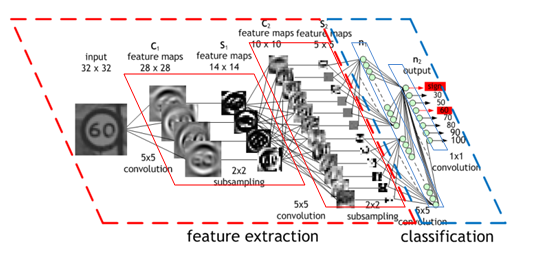
\includegraphics[width=0.9\linewidth]{img/cnn}
	\caption{Aufbau eines CNN zur Klassifizierung am Beispiel zur Erkennung einer Zahl auf einem Straßenschild. Bild von \cite{bild_CNN}}
	\label{img_cnn}
\end{figure}
\newpage
\subsection{Constrained Local Model (CLM)}
In Constrained Local Modellen wird die Erkennung eines Objektes in die Erkennung einzelner charakteristischer Teilpunkte, der sogenannten Landmarks, aufgespalten. Dieses Verfahren eignet sich deshalb besonders dazu deformierbare Objekte zu erkennen.\\
Um mehrere Punkte eines Objektes zu lokalisieren wird eine Wahrscheinlichkeitskarte der einzelnen Teilpunkte relativ zueinander gelernt. Auf dem Eingabebild wird dann die Ähnlichkeit der Bildregionen mit den gesuchten Punkten quantifiziert, die die Ähnlichkeit der Darstellung angibt. Anschließend wird die optimale Kombination aus Bildähnlichkeit und der Lage aller Punkte zueinander bestimmt.\\
Diese Art der Bestimmung von positionsabhängigen Punkten ist ziemlich zuverlässig und dennoch dynamisch genug um auch mit kleinen Veränderungen zurecht zu kommen.\\
Dies ist wichtig bei der Detektion von leicht verformbaren Objekten wie beispielsweise Gesichtern und ist zuverlässiger als das Active Appearance Model (AAM).
\cite{pdf_CLM}
\subsection{Constrained Local Neural Fields (CLNF)}
Bei CLNF handelt es sich um einen Gesichtsdetektor. Für die Detektion wird für jedes Merkmal ein eigener Detektor eingesetzt der auf einem Bildbereich arbeitet und eine Wahrscheinlichkeitskarte für dieses Merkmal erstellt.\\
Als nächster Schritt werden die Ergebnisse der Detektoren mit einer Karte der Position aller Landmarks, entsprechend dem Vorgehen eines CLM, verglichen.
\cite{CLNF}
\subsection{Active Appearance Model (AAM)}
Dies ist ein Verfahren der Bildverarbeitung um Übereinstimmungen zu einem Modell zu finden. Dazu wird aus dem Trainingsdatensatz eine typische \glqq durchschnittliche\grqq Form eines Objektes, sowie die Faktoren der wichtigsten möglichen Veränderungen der Form ermittelt. So können beispielsweise alle Merkmale, die ein Gesicht als männlich oder weiblich charakterisieren in einem Abweichungsvektor zusammengefasst und durch einen einzigen Gewichtungsparameter beschrieben werden.\\
Soll nun zu einem Eingabebild die Übereinstimmung ermittelt werden, so müssen nur die wichtigsten Veränderungsfaktoren angepasst werden. Dies ist ein bedeutend kleinerer Parameterraum als alle Landmarks einzeln anzupassen. Sind dennoch Unterschiede zur Eingabe vorhanden, liegen diese an der Erscheinung des Objektes.
\cite{wiki_AAM}
\subsection{Patch Experts}
Das Patch Experts ist ein Bewertungsverfahren um die Wahrscheinlichkeit zu ermitteln, dass ein Landmark an einer bestimmten Stelle im Bild dargestellt wird. Für die Bestimmung wird ein ganzer Bereich um diese Position herum ausgewertet, um Ergebnisse auf ein Teilpixels genau zu bestimmen.
\cite{CLNF}
\subsection{Non-maximum suppression  (NMS)}
Das NMS ist ein Verfahren um ein lokales Maximum zu bestimmen und kann z.B. in einem Bild eingesetzt werden um Kanten exakter zu bestimmen.\\
Als Eingabe für das Verfahren zur exakten Bestimmung einer Kante, wird das Ergebnis eines Kantendetektor z.B. Kirsch-Operator verwendet. Dabei gibt die Höhe des Farbwertes eines Pixels an, wie nahe es an einer Kante im Originalbild liegen. Bei der Verarbeitung wird nun der Farbwert jedes einzelnen Pixels des Eingabebildes mit seinen umliegenden verglichen und sollte dieser Wert nicht maximal sein auf Null gesetzt.\\
Auf diese Weise bleibt nur noch ein Kantenpixel übrig. Wird das Verfahren auf die Bestimmung von Boxen eingesetzt, so wird jene Fläche bestimmt die von allen am ehesten beschreiben wird.
\cite{NMS}\cite{wiki_Canny}
\subsection{Point Distribution Model (PDM) \& Generalized Adaptive View-based Appearance Model (GAVAM)}
Mit einem Point Distribution Model (PDM) können verformbare Objekte modelliert werden. Dabei wird die durchschnittliche Form $\overline{X}$ des Objekts anhand der Eingabe bestimmt und eine Matrix $P$ von Eigenvektoren ermittelt, um die möglichen Deformierungen darzustellen.
\begin{align*}
X &= \overline{X}+P\cdot b
\end{align*}
Somit können durch einen Skalierungsvektor $b$ alle möglichen Eingabeformen $X$ des Objektes aus dem Durchschnittsmodell wiederhergestellt werden. Zur Vereinfachung reicht es, die signifikantesten Eigenvektoren in $P$ aufzunehmen und dennoch $X$ ausreichend genau beschreiben zu können.\\
Ist bekannt welche Art der Verformung durch den Eingenvektor dargestellt wird, z.B. eine bestimmte Orientierung, so kann anhand des Skalierungsvektors die Rotation der Eingabe bestimmt werden, siehe Generalized Adaptive View-based Appearance Model (GAVAM).\\
Eine Problematik bei dieser Art der Rotationsbestimmung entsteht, wenn die Lösung nicht eindeutig ist. Dies kann daran liegen, dass unter Umständen durch verschiedene Gewichtungskombinationen die selbe Darstellung erzielt wird oder dass eine nicht erfasste Verformung des Objektes stattgefunden hat, wodurch immer eine Abweichung zu allen Kombinationen entsteht.\\
Dieses Problem der Verformung tritt bei Berechnungen von Gesichtern auf, da immer eine Veränderung z.B. der Mundwinkel oder Augenlider vorhanden ist.
\cite{pdf_PDM}\cite{pdf_GAVAM}\cite{wiki_PDM}
\section{MTCNN Face Detection}
\label{MTCNN}
Bei Multi-task Cascaded Convolutional Network handelt es sich um ein Verfahren dass bei der Detektion von Gesichtern auch deren Ausrichtung berücksichtigt wird, um so bessere Ergebnis zu erzielen.
\subsection{Anforderungen}
Sein Einsatzgebiet ist die Vorverarbeitung eines Frames für die spätere Auswertung. Somit soll dieser Schritt von einem möglichst robusten Verfahren zur Detektion von Gesichtern durchgeführt werden.\\
Dabei wird auf recht großen Bild gearbeitet mit verhältnismäßig kleinen und verschieden großen Gesichtern.\\
Außerdem sollte das Verfahren ausreichend schnell sein, da es sich hierbei nur um ein Vorverarbeitungsschritt handelt und zur Beschleunigung der späteren Berechnung beitragen soll.
\subsection{Die 3 Stufen der Verarbeitung}
Für die gute Detektionsqualität sorgt die dreistufige Verarbeitung auf der Bildpyramide. Bei der Bildpyramide handelt es ich um ein in verschiedenen Größen skaliertes Bild, damit der Gesuchte Inhalt in der gewünschten Auflösung abgebildet ist, ohne dass etwas über den Inhalt bekannt ist.\\
Dies ist von Vorteil, damit das CNN auf eine feste Größe von Gesichtern optimiert werden kann, um neben dem möglichen Farbverläufen, durch die Skalierung das Lernen nicht zusätzlich zu erschweren.
\begin{figure}
	\centering
	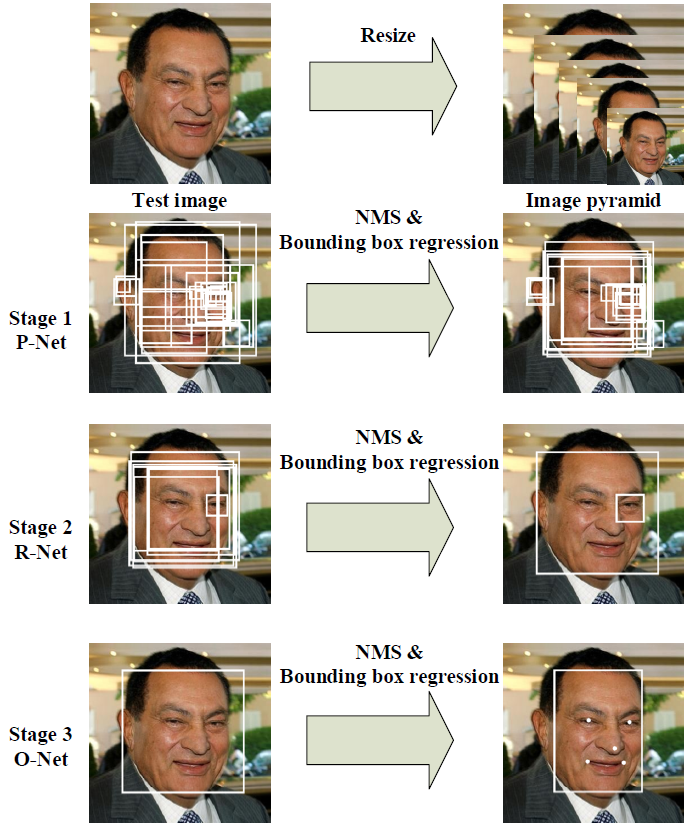
\includegraphics[width=0.5\linewidth]{img/MTCNN_Step}
	\caption{Darstellung des Funktionsablaufes von MTCCN\cite{MTCCN}}
	\label{img_MTCNN_Step}
\end{figure}
\subsubsection{Stufe 1}
Beim ersten Verarbeitungsschritt erden alle Bereiche eines Bilds gesucht, in denen möglicherweise ein Gesicht zu sehen ist. Dazu wird zuerst ein einfaches CNN eingesetzt und die Ergebnisse, die sich sehr stark überlappen, zusammengefasst.\\
Für die Detektion wird von einem CNN, dem sogenannte Proposal Network (P-Net), eingesetzt und sehr viele Bounding-Boxen ermittelt. Diese werden nun mit einem NMS ausgedünnt, um die am stärksten überlappenden Bounding-Boxen zusammen zu fassen.
\subsubsection{Stufe 2}
Anschließend werden die möglichen Bereiche mittels eines weiten CNN analysiert, damit alle Nicht-Gesichtsbereiche erkannt und entfernt werden können.\\
Dies wird von dem Refine Network (R-Net) übernommen und anschließend die möglichen Bounding-Boxen mittels NMS weiter reduziert.
\subsubsection{Stufe 3}
Der letzte Schritt wird von einem deutlich genaueren CNN übernommen, um ein Gesicht zu detektieren, dem sogenannten Output Network (O-Net). Womit die resultierenden exakten Boxen und 5 Landmarks ermittelt werden.
\subsection{Qualität}
MTCNN Face Detection ist bei der Zuverlässigkeit im Verglich zu anderen bekannten Verfahren überlegen, siehe \autoref{img_MTCNN_quality} und zudem Echtzeit fähig. Im Test-Datensatz sind auch Gesichtern mit einer Größe von $20\times 20$ enthalten und wurden erfolgreich erkannt.\\
Somit sind alle Anforderungen erfüllt um mit diesem Verfahren den vorhanden Frame für die nachfolgenden Berechnungen vorzubereiten, daher wird es auch hier eingesetzt.
\begin{figure}
	\centering
	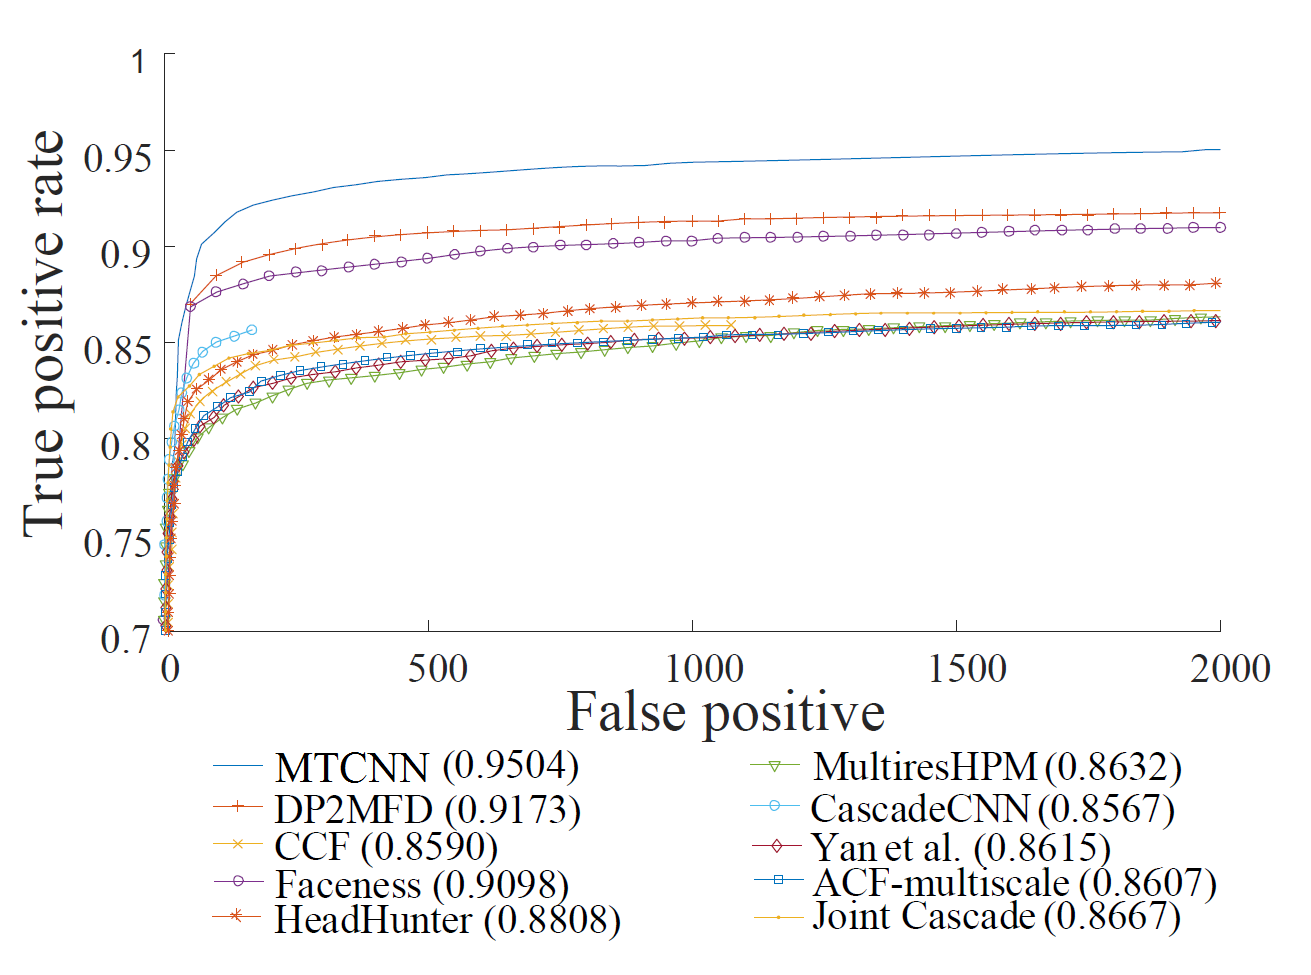
\includegraphics[width=0.5\linewidth]{img/MTCNN_quality}
	\caption{normale blaue Linie\cite{MTCCN}}
	\label{img_MTCNN_quality}
\end{figure}
%Joint Face Detection and Alignment using Multi-task Cascaded Convolutional Networks
\subsection{Skalieren von Bildern}
Da die Berechnungen meist auf recht kleinen Bildausschnitten ausgeführt werden muss, müssen diese für die weiteren Rechenschritte Hochskaliert werden.\\
Dabei ist es wichtig, dass die Gesichtsmerkmale möglichst gut rekonstruiert werden damit die entsprechenden Landmarks gefunden und bestimmt werden können.
\subsubsection{Nearest-Neighbor}
Verwende gleicher Farbwert wie das Nächstgelegene Pixel. Dadurch werden nur die ehemaligen Pixel größer und das Gesicht wirkt sehr Kantig.\\
To Do! - Bsp Bilder
\subsubsection{Linear}
Dabei wird zwischen den umliegenden nächst gelegenen Pixel Interpoliert, wodurch weitere Farbwerte entstehen und das Ergebnis gleichmäßiger aber unscharf wirkt.
To Do! - Bsp Bilder
\subsubsection{Bicubic}
Um den Farbwert zu ermitteln, werden die umliegenden $4\times 4$ Pixelwerte betrachtet um den Farbverlauf als eine Funktion 3. Grades zu bestimmen. Somit werden feinere Details besser dargestellt als beim Linearen verfahren, allerdings kann es durch den bestimmten Verlauf auch zum Überschwingen kommen, wodurch Fehlfarben entstehen können.\\
To Do! - Bsp Bilder
%%https://en.wikipedia.org/wiki/Bicubic_interpolation
\subsubsection{Lanczos}
Dieser Filter besteht aus einer Sinc-Funktion über einen Bereich, um so eine Bewertung der Benachbarten Pixelwerte zu erhalten. Somit kann ergibt sich der Neue Farbwert aus den bewerteten umliegenden Pixeln.\\
To Do! - Bsp Bilder
%%To Do! - Bsp Bilder

%% http://docs.opencv.org/2.4/modules/imgproc/doc/geometric_transformations.html#resize
\section{OpenFace}
Die Aufgaben von OpenFace ist die Analyse der Gesichtes aus Bildern. Dabei sind nur die Kameraparameter bekannt und keinerlei Zusätze wie eine Tiefenbild oder Infrarotbeleuchtung der Szene. Dabei ist für die Anwendung die Kopfposition (Translation und Orientierung) und Blickrichtung von Interesse, da mit ihnen zurückrechnet werden kann wohin der Schüler schaut.\\
OpenFace kann neben den Landmarks auch die Position, Blickrichtung und Gesichtsmerkmale bestimmen, basierend auf einem einfachen Bild. Sollte ein Video als Quelle fungieren, so kann OpenFace auch lernen. 
\subsection{Verarbeitungsschritte}
Der Rechenaufwand ist so ausgelegt, dass alle Berechnungen auf einer Webcam in Echtzeit ausgeführt werden können, dies ist im aktuellen Fall nicht notwendig, da es sich um eine nachträgliche Auswertung handelt. Durch den Aufbau sind nur recht kleine Farbbilder der Gesichter in einem Video vorhanden wodurch eine Auswertung erschwert wird.
\subsubsection{Gesichts-Landmarks: Detektion und Verfolgung}
Für die Bestimmung und Tracking der Landmarks wird ein Conditional Local Neural Fields (CLNF) eingesetzt. Dabei Handels es sich im Grunde um ein Constrained Local Model (CLM) nur mit verbesserter Patch Experts und Optimierungsfunktionen.\\
Zu Beginn werden verschiedene initiale Hypothesen aus dlib-Bibliothek verwendet und die Passende ausgewählt. Bei den initiale Hypothesen handelt es sich um verschiedene Gesichtsorientierungen auf denen verschiedene Netze gelernt wurden. Dies ist zwar langsamer, aber auch exakter als eine einfache Hypothese.\\
Wird ein Tracing auf Videos gemacht, so wird als initiale Hypothese das Ergebnis aus dem letzten Frame verwendet.\\
Sollte das Tracing scheitern, so wird das CNN reseted um Neu zu beginnen.
Die beiden Hauptkomponenten ist das Point Distribution Model (PDM) zur Erfassung der Anordnung der Landmarks und patch experts zum Erfassen der Variante der einzelnen Landmarks.\\
Auf diese weise werden 68 Gesichts-Landmarks und  weitere 28 pro Auge erfasst. Zur Brechung auf den Gesichtern sollte es eine Mindestbreite von 100 Pixeln für eine zuverlässige Detektion Originalgröße besitzt.
\subsubsection{Bestimmung der Gesichtsposition}
Zur Bestimmung der Translation und Orientierung des Gesichtes wird ein CLNF eingesetzt. Dabei wurde es mit der Kameraabbildung der 3D-Landmarks eines Kopfes in verschiedenen Positionen initialisiert. Womit auf eine Normierte Abbildung berechnet wird, diese kann mit den passenden Kameraparameter für die Aufnahme angepasst werden um die reale Position zu bestimmen. Sind keine bekannt, so können diese geschätzt werden.\\
Bei der Schätzung der Brennweite für ein Bild mit einer Dimension $I_x\times I_y$ wird das Standardobjektiv mit 50 mm und einer Auflösung von $640 \times 480$ Pixel angenommen, somit ergibt sich für die Brennweiten $f_x$ und $f_y$:
\begin{align*}
f_x = 500\cdot \frac{I_x}{640}\\
f_y = 500\cdot \frac{I_y}{480}
\end{align*}
\subsubsection{Bestimmung der Blickrichtung}
Durch die Landmarks der Augen werden die Augenlider, Iris und Pupille dargestellt und für jedes Auge separat bestimmt. Dabei wird der Augenbereich, basierend auf dem Gesicht, verwendet um mit einem weiten CNN die 28 Landmarks zu bestimmen.\\
Zur Bestimmung der Blickrichtung wird wie folgt vorgegeben. Zuerst wird der Strahl bestimmt der, ausgehend vom Zentrum der Kamera, durch das Zentrum der Pupille verläuft. Nun wir der Schnittpunkt zwischen diesem Strahl und einer Sphäre bestimmt, die das Auge repräsentiert. Nun wird ein Strahl bestimmt der vom Zentrum der Sphäre ausgehend durch den berechneten Schnittpunkt verläuft, dies ist die resultierende Blickrichtung.
\subsubsection{Detection der Gesichtsmerkmale}
Dieser Schritt kann von OpenFace ausgeführt werden, ist aber  im aktuellen Fall nicht von Relevanz.
\subsection{Veröffentlichte Genauigkeit}
Die Messung wurde auf de Biwi Kinect head pose dataset und BU dataset. Für die Genauigkeit der Kopfposition haben sich folgend Werte ergeben in Grad:\\
\begin{tabular}{|l|c|c|c||c|c|}
	\hline
	&Yaw&Pitch&Roll&Mean&Median\\\hline
	Biwi Kinect \cite{BIWI_database}&7.9&5.6&4.5&6.0&2.6\\\hline
	BU dataset \cite{BU_database}&2.8&3.3&2.3&2.8&2.0\\\hline
	ICT-3DHP \cite{ICT_database} &3.6&3.6&3.6&3.6&-\\\hline
\end{tabular}\\\\
Für die Qualität zur Bestimmung der Blickrichtung ergab sich ein durchschnittlichen Fehler von 9.96 Grad.
\section{Graukonvertierung: Farbbild nach Graubild}
\label{Graubild}
Da die Berechnungen von ElSe auf Graubildern arbeitet und das Eingabebild in Farbe ist, muss es in ein Graubild umgewandelt werden.\\
Die Wahl des Verfahrens beruht auf der Anforderung von ElSe, dass vor allem der Farbunterschied zwischen Pupille und der Umgebung maximal sein soll, die Pupille möglichst dunkel und das restliche Auge hell. Die Farbe der Iris erschwert die Differenzierung zusätzlich, wenn diese recht dunkel ausfällt ist auch der Unterschied zur Pupille entsprechend gering in den Grauwerten. Außerdem ist das Erkennen der Pupille bei sehr kleinen Bildern schwierig bis unmöglich wodurch auf der Iris gerechnet werden muss, und daher diese weiterhin erhalten bleiben sollte.\\
Nach der Umwandlung wird für die Anwendung das Graubild noch normiert, damit mindestens ein schwarzes und ein weißes Pixel vorhanden ist.\\
Die Wahl von Gleam basiert auf den Ergebnissen von \glqq Color-to-Grayscale: Does the Method Matter in Image Recognition?\grqq \cite{rgb_to_Gray} und New-Gleam als eine Umsetzung des dort veröffentlichtem Ausblicks. Luminance als Standart , Quadrat als gegenstück zu Gleam und Min/Max beruht auf der Idee die farbigen Iris zu nutzen.\\
Das Eingabebild der Beispiele der einzelnen Graukonvertierung ist in \autoref{img_Gray_Einagbe} dargestellt. Eine Farbpalette, das Bildverarbeitungsbeispiel Lena sowie ein Augenbereich aus dem Augendatensatz \cite{database_Eye}. 
\begin{figure}
	\centering
	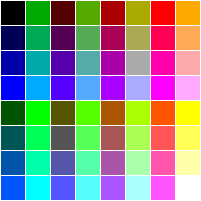
\includegraphics[width=0.2\linewidth]{img/Farbtafel2}
	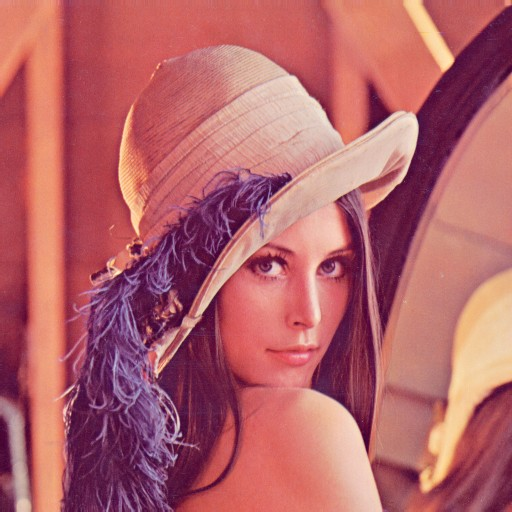
\includegraphics[width=0.2\linewidth]{img/lena}
	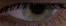
\includegraphics[width=0.2\linewidth]{img/Auge}
	\caption{Dies sind die Eingabebilder der verschiedenen Konverter von Farbe nach Grau. Links eine Farbpalette, Mitte Lena und Rechts ein Augenausschnitt aus dem Augendatensatz \cite{database_Eye}}
	\label{img_Gray_Einagbe}
\end{figure}
\subsection{Gleam-Verfahren}
\label{gray_Gleam}
Bei dem Gleam-Verfahren wird jede Farbe (Rot,Gelb und Grün) gleich stark bewertet allerdings wird jeder Farbwert mittels einer Gamma-Korrektur verändert und das Bild wirkt heller als bei dem Luminance-Verfahren.\\
Durch die Gamma-Korrektur wird vor allem der helle Bereich weiter erhöht, somit wird der Farbunterschied zwischen Iris und Auge vermindert, wodurch die Pupille der einzige dunkle Bereich wird, siehe \autoref{img_Gleam}.\\
Allerdings wird auch dieser Farbwert erhöht und sollte die Pupille nicht schwarz sein, wird sie eher ins Graue überführt.\cite{rgb_to_Gray}\\
\[G_{Gleam}=\dfrac{R^{\frac{1}{2,2}} + G^{\frac{1}{2,2}} + B^{\frac{1}{2,2}}}{3}\]
\subsection{Gleam-New-Verfahren}
\label{gray_New}
Dies ist eine Variante von Gleam bei dem zuerst das gesamte Bild analysiert wird um die Parameter für die jeweilige Gamma-Korrektur zu ermitteln. Dies ist etwas aufwendiger, aber für die kleinen Bilder hinnehmbar.\\
Durch die individuelle Veränderung der Farbkanäle, werden Farbunterschiede minimiert und somit alle stark farbigen Bereiche ebenfalls dunkel dargestellt. Der Kontrast zwischen der farbigen Iris und dem weißen Auge wird verbessert, siehe \autoref{img_NewGeam}.\\
Da allerdings alle Farben dunkel werden, entstehen weitere dunkle Bereiche die die Detektion der Pupille beeinträchtigen können.
\[G_{Gleam-New}=\dfrac{R^{r} + G^{g} + B^{b}}{3}\]
Wobei gilt $\{r,g,b\} = \frac{\log(V_{\max})}{\log(\{R,G,B\}_{\max})}$ mit $V_{\max}$ als maximal möglicher Farbwert und $R_{\max}$ als maximal Vorhandener Rot-Wert, $G_{\max}$ und $B_{\max}$ äquivalent.
\subsection{Luminance-Verfahren}
\label{gray_Luminance}
Dies ist ein lineares Verfahren, das der menschlichen Farbwahrnehmung entspricht und oft den Standard bei der Umwandlung von Farbbild nach Graubild darstellt. Somit entsteht ein natürlicher Farbverlauf, bei dem der Farbunterschied zwischen Pupille, Iris und Auge auf einem mittleren Niveau bleibt, siehe \autoref{img_Luminance}.\\
Eine Gamma-Korrektur wird bei der Umwandlung nicht verwendet.\cite{rgb_to_Gray}
\[G_{Luminance} = 0,299 R + 0,587 G + 0,114 B\]
\subsection{Min-Max-Verfahren}
\label{gray_MinMax}
Dabei handelt es sich eigentlich um zwei verschiedene Varianten, allerdings funktionieren beide nach dem selben Prinzip. Als Grauwert wird der jeweilige Extremwert aus den einzelnen Farbkanälen des Pixels gewählt.\\
Durch Verwendung der Extremwerte, ist nur noch der Wert von Relevanz, nicht die eigentliche Farbe, wodurch das gesamte Bild deutlich heller bzw. dunkler wird.\\
Bei dem Max-Verfahren werden alle farbigen und helle Bereiche hell dargestellt und nur gleichmäßig dunkel Bereiche bleiben dunkel wie es bei schwarz der Fall ist. Wenn der Minimalwert anstelle verwendet wird, bleiben nur gleichmäßig helle Bereiche hell, alle anderen werden abgedunkelt.
\begin{align*}
G_{Max} &= \max(R,G,B)\\
G_{Min} &= \min(R,G,B)
\end{align*}
\subsection{Quadrat-Verfahren}
\label{gray_Quadrat}
Dies ist ein Verfahren, dass das Eingabebild verdunkelt und vom Aufbau dem Inversen von Gleam entspricht. Somit ist das gesamte Bild dunkler als bei dem Luminance-Verfahren, siehe \autoref{img_Quadrat}.\\
Durch die Abdunklung werden kleine Farbänderungen in den dunklen Bereichen reduziert, wodurch die Pupille sehr dunkel und der Farbunterschied zur Iris geringer ausfällt.
\[G_{Quadrat}=\dfrac{R^2+G^2+B^2}{3}\]
\subsection{Normalisierung der Graubilder}
Um ein Graubild zu erhalten, das das volle Spektrum der möglichen Grauwerte erfüllt, wird das Eingabebild normalisiert. Dazu wird der Maximale $G_{max}$ und Minimale $G_{min}$ Grauwert im Bild gesucht. Anschließend wird der neue Grau-Wert $G_{new}$ wie folgt bestimmt:
\[G_{new} = (G-G_{min})\cdot \dfrac{V_{max}}{G_{max}-G_{min}}\]
Dabei ist $V_{max}$ der maximale mögliche Wert in der Ausgabe und $G$ der aktuelle Grauwert im Bild.\\
Da für die Anwendung ein schwarzer Bereich gegen einen hellen Hintergrund gesucht wird, wird für die Bestimmung der Extremwerte nicht das originale Bild verwendet, sonder ein Gauß-gefiltertes.\\
Dies hat den Vorteil, dass einzelne lokal auftretende Werte, z.B. Reflektionen, nicht als Extremwert verwendet werden, wodurch die Pupille gleichmäßiger dunkler und das gesamte Bild stärker aufgehellt wird.\\
Der Gauß-Filters ist ein Tiefpassfilter und wird verwendet um das Eingangssignal zu glätten. Dies hat in der Bildverarbeitung den Effekt, dass Details im Bild verschwimmen und das Bild unscharf wirkt.\\
Die einzelnen Werte werden ihrer Umgebung angepasst, wodurch lokal auftretende Extremar verschwinden bzw. abgeschwächt werden und ähnliche Farbwerte zu ihrer Umgebung erhalten bleiben.
\begin{figure}
	\centering
	
\includegraphics[width=0.2\linewidth]{img/Farbkarte2}
	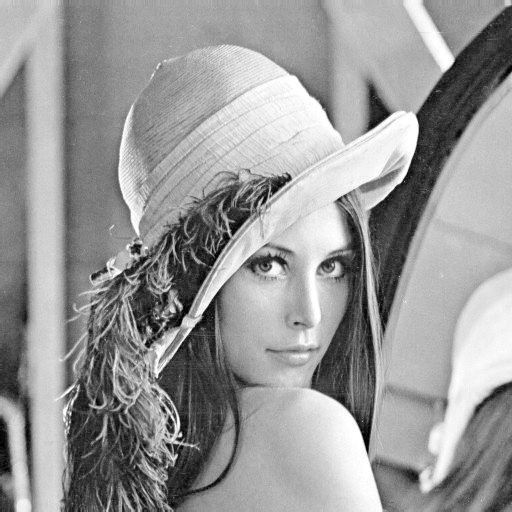
\includegraphics[width=0.2\linewidth]{img/Lena2}
	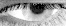
\includegraphics[width=0.2\linewidth]{img/Auge_2Gray}
	\caption{Ergebnis der Umwandlung von Farb- nach Grauwert mittels Gleam-Verfahren}
	\label{img_Gleam}
\end{figure}
\begin{figure}[p]
	\centering
	
\includegraphics[width=0.2\linewidth]{img/Farbkarte1}
	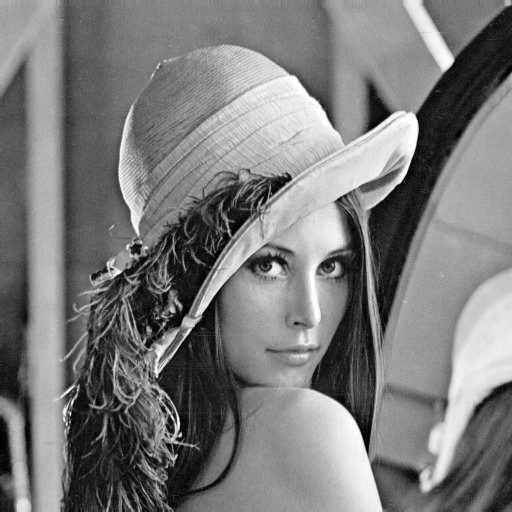
\includegraphics[width=0.2\linewidth]{img/Lena1}
	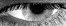
\includegraphics[width=0.2\linewidth]{img/Auge_1Gray}
	\caption{Ergebnis der Umwandlung von Farb- nach Grauwert mittels Gleam-New-Verfahren}
	\label{img_NewGeam}
\end{figure}
\begin{figure}[p]
	\centering
	
\includegraphics[width=0.2\linewidth]{img/Farbkarte0}
	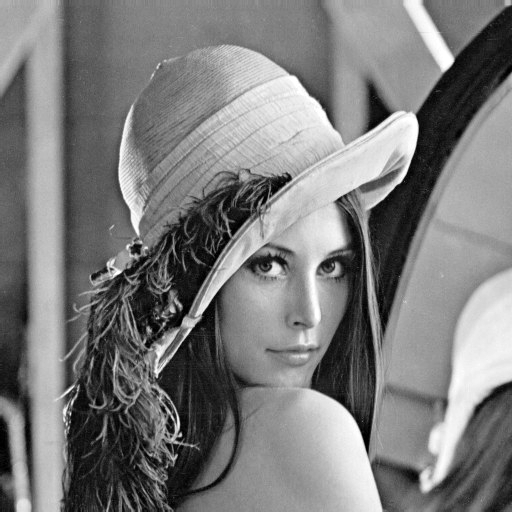
\includegraphics[width=0.2\linewidth]{img/Lena0}
	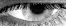
\includegraphics[width=0.2\linewidth]{img/Auge_0Gray}
	\caption{Ergebnis der Umwandlung von Farb- nach Grauwert mittels Luminance-Verfahren}
	\label{img_Luminance}
\end{figure}
\begin{figure}[p]
	\centering
	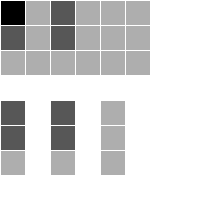
\includegraphics[width=0.2\linewidth]{img/Farbkarte5}
	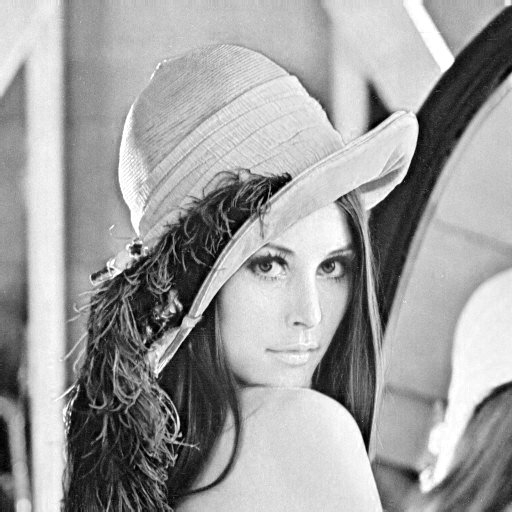
\includegraphics[width=0.2\linewidth]{img/Lena5}
	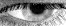
\includegraphics[width=0.2\linewidth]{img/Auge_5Gray}\\
	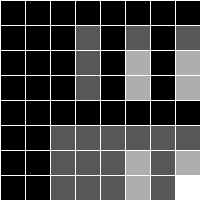
\includegraphics[width=0.2\linewidth]{img/Farbkarte4}
	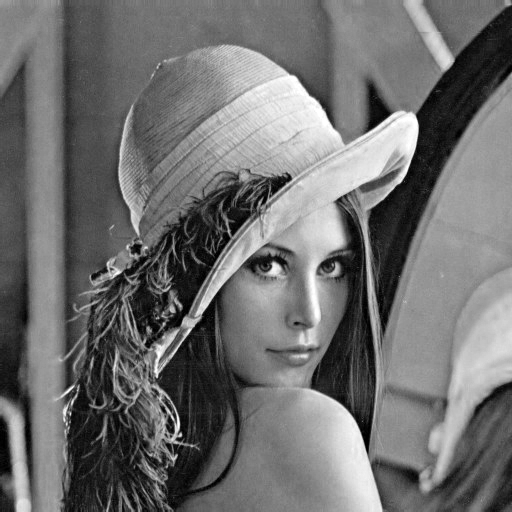
\includegraphics[width=0.2\linewidth]{img/Lena4}
	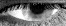
\includegraphics[width=0.2\linewidth]{img/Auge_4Gray}
	\caption{Ergebnis der Umwandlung von Farb- nach Grauwert mittels Extremwert-Verfahren. Oben: Max-Verfahren, Unten: Min-Verfahren}
	\label{img_MinMax}
\end{figure}
\begin{figure}[p]
	\centering
	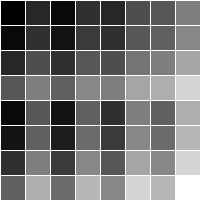
\includegraphics[width=0.2\linewidth]{img/Farbkarte3}
	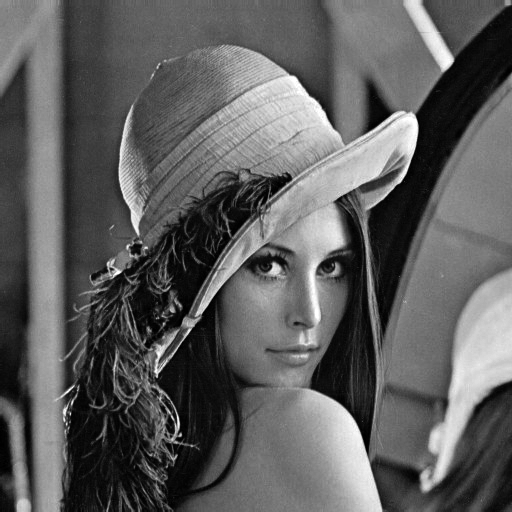
\includegraphics[width=0.2\linewidth]{img/Lena3}
	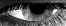
\includegraphics[width=0.2\linewidth]{img/Auge_3Gray}
	\caption{Ergebnis der Umwandlung von Farb- nach Grauwert mittels Quadrat-Verfahren}
	\label{img_Quadrat}
\end{figure}
\section{Augenanalyse mit Ellipse Selection for Robust Pupil Detection (ElSe)}
\label{ElSe}
Zur Bestimmung der Blickrichtung ist die Augenregion natürlich von besonderer Bedeutung. Aus diesem Grund werden die Landmarks der Augenregion nochmals gesondert betrachtet. Aufgrund der besonderen Bedeutung existiert eine große Anzahl an Algorithmen, die speziell auf eine hochgenaue Bestimmung von Augenmerkmalen optimiert sind, wie beispielsweise ElSe \cite{ElSe}, Goutam \cite{Eye_FastCorner}, Starburst \cite{Starburst} oder Swirski \cite{Swirski2012}. Auch OpenFace verwendet ein zusätzlich dafür trainiertes CLNF, um weiter 28 LAndmarks pro Auge zu bestimmen, zusätzlich zu den 64 Landmarks das Gesicht. Aus diesen Augen-Landmarks, die Lider, Iris und Pupille dargestellen kann die Blickrichtung ermittelt werden.\\
Um die Position der Landmarks zu verbessern, kann auf den Augenbereichen der ElSe-Algotithmus eingesetzt werden. Dieser Algorithmus basiert auf einem rechnerischen Ansatz und nicht auf Neuronen um die Umrisse der Pupille zu berechnen. Für die Verbesserung wurde das ElSe-Verfahren wurde gewählt, da es im Test \cite{ElSe} am besten abgeschnitten hat und direkt das Zentrum der Pupille liefert.\\
Der ursprüngliche ElSe-Algorithmus ist für Graubilder einer Eye-Tracking-Brille ausgelegt und optimiert, zudem ist es auf diesen Bildern zu einer Echtzeitauswertung in der Lage. Dieser Anwendungsbereich betrifft vor allem die Anforderung an eine hohe Qualität der Aufnahme im Bezug auf die Auflösung und der Infrarotbeleuchtung des Bildes. Die Infrarotbeleuchtung wird verwendet, damit das Auge ausreichend beleuchtet ist ohne den Probanden zu blenden. Diese Voraussetzungen führen dazu, das die Detektionsleistung bei niedriger auflösenden Bildern rasch abnimmt.\\
Als Ergebnis liefert ElSe eine Ellipse, die den Umriss der Pupille im Bild beschreibt. Aus dieser Ellipse können die Landmarks der Pupille abgeleitet werden.\\
Für den Test im Paper wurden Bilder von $384\times 288$ Pixel Größe verwendet und im Vergleich zu den anderen Verfahren ist ElSe in den meisten Fällen überlegen, mit einer Verbesserung der Erkennungsrate um $14.53\%$ auf dem verwendeten Datensatz.\cite{ElSe}\\
Für die Anwendung wurde der ursprüngliche ElSe-Algorithmus angepasst, um auf Farbbildern die nach Grau konvertiert wurden arbeiten zu können.
\subsection{Pupille bestimmen mit Kantendetektion}
Da die Pupille als schwarzen Fleck im Bild dargestellt ist und die Iris einen helleren Farbton aufweist, wird ein Kantendetektor verwendet, der alle Pixel markiert, bei denen eine starke Farbänderung auftritt. Bei ElSe wird ein morphologischen Ansatz eingesetzt, von Relevanz sind nur zusammenhängende Kantenpixel um die Kante zwischen Pupille und Iris zu finden. Alle anderen Pixel können ignoriert werden, wobei jedes Kantenpixel als Startpunkt der Berechnung dienen kann.\\
Um jene Kantenpixel zu erhalten, die die Pupille beschreiben, wird versucht fortlaufende Kanten zu finden, die eine Ellipse bilden. Jene die nicht diesen Anforderungen entsprechen, können recht schnell ignoriert werden. Anschließend werden auch alle offenen Ellipsenverläufe und jene Kantenpixel die am meisten vom bestimmten Verlauf abweichen, verworfen.\\
Das beste Ergebnis aller bestimmten Ellipsen wird als Lösung verwendet.
\subsection{Grobe Bestimmung der Pupille}
\label{ElSe_Grob}
Sollte die Bestimmung der Ellipse, wie im vorigen Kapitel beschreiben, scheitern, so wird das Zentrum des dunkelsten Kreises ermittelt. So ein Punkt kann immer gefunden werden, ist aber nicht zwingend die Pupille.\\
Auf einem verkleinerten Bild, \autoref{img_else} (1), wird ein kreisförmiger Mean-Filter eingesetzt mit Ergebnis in \autoref{img_else} (3). Zur zweiten Faltung wird der Durchschnitt über ein Quadrat ohne inneren Kreis eingesetzt mit Ergebnis in \autoref{img_else} (2), wobei für beide Kreisen der selbe Radius verwendet wird.\\
Nun wird das Ergebnis des Quadratischen Mean-Filters invertiert, \autoref{img_else} (4), und mittels Punkt-Multiplikation mit dem anderen Meanfilter zusammengebracht, \autoref{img_else} (5). Im resultierendem Bild wird nun der höchste Wert gesucht, da dies das Zentrum des dunkelsten kreisförmigen Ortes im Bild ist.\\
Ergebnis des Beispiels ist als Kreuz in \autoref{img_else} (6) markiert. 
\begin{figure}
	\centering
	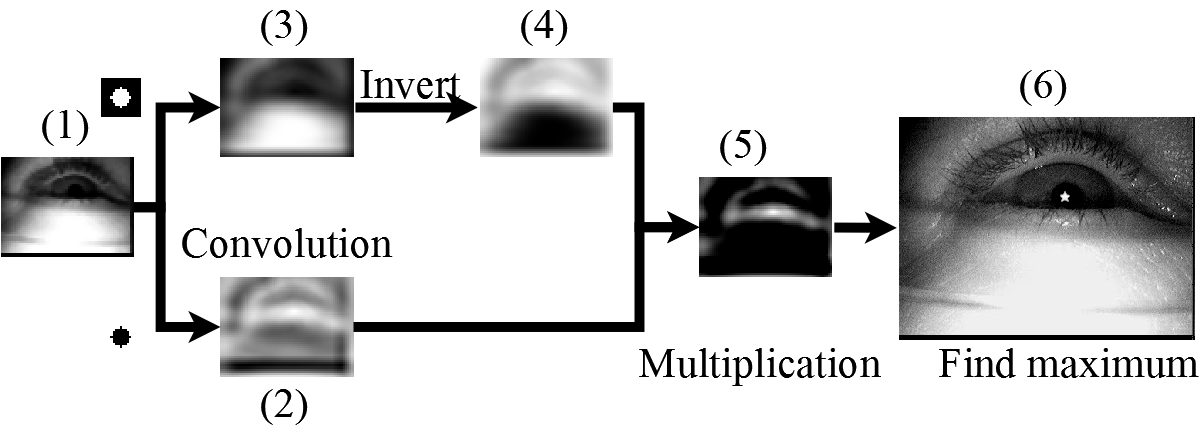
\includegraphics[width=0.8\linewidth]{img/ElSe}
	\caption{Ablauf der alternativen Berechnung zur Pupillen-Detektion von \cite{ElSe}}
	\label{img_else}
\end{figure}
\section{Bestimmung des Ziels der Aufmerksamkeit}
\label{calc_Position}
Um das Ziel der Aufmerksamkeit einer Person zu bestimmen, muss die 3D-Position ermittelt werden. Die Orientierung des Gesichtes und die Blickrichtung können als Verlauf einer Ursprungsgerade betrachtet werden, mit dem Ursprung an der Position des Gesichtes im Raum.\\
Ist der Ursprung und die Gerade bekannt, so kann ermittelt werden, ob die Gerade durch bestimmte Punkte im Raum verläuft. Ist dies der Fall, so wird dieser Punkt wahrscheinlich betrachtet und ist Ziel der Aufmerksamkeit der Person.
\subsection{Bestimmung der Position \& Orientierung des Gesichts}
Zur Bestimmung der Translation und Orientierung des Gesichtes wird ein CLNF bzw. PDM eingesetzt. Dabei wurde es mit der Kameraabbildung von 3D-Landmarks eines normierten Kopfes in verschiedenen Ausrichtungen initialisiert. Das normierte Ergebnis kann mit den passenden Kameraparametern der Aufnahme angepasst werden, um die reale Position und Orientierung zu bestimmen.
\subsubsection{Abschätzen der Kameraparameter}
Sind keine Kameraparameter bekannt, so können diese anhand der Bildauflösung grob geschätzt werden. Bei der Schätzung der Brennweite für ein Bild mit einer Dimension $I_x\times I_y$ wird das Standardobjektiv mit einer Auflösung von $640 \times 480$ Pixel angenommen, somit ergebenen sich die Brennweiten $f_x$ und $f_y$ wie folgt \cite{OpenFace}:
\begin{align*}
f_x = 500\cdot \frac{I_x}{640}\\
f_y = 500\cdot \frac{I_y}{480}
\end{align*}
\subsubsection{Position \& Orientierung}
\label{OpenFace_Pos_Ori}
Zur Bestimmung der Kopfposition $P= \begin{pmatrix}
X_{avg} & Y_{avg} & Z_{avg}
\end{pmatrix}^t$ im Kamerakoordinatensystem wird die Größe, ein Skalierungsfaktor der normierten Kopfgröße $S_G$, im Bild verwendet.\\
Bei der Abbildung von Welt- nach Bild-Koordinaten gilt: $x=f\cdot \frac{X}{Z}$ und $ y=f\cdot \frac{Y}{Z}$, damit kann die Tiefe abgeschätzt werden.\\
Sei $P_1 = \begin{pmatrix}
X_1&Y_1&Z_1
\end{pmatrix}^t, P_2= \begin{pmatrix}
X_2&Y_2&Z_2
\end{pmatrix}$ die Beschreibung der Größe $G$ eines Kopfes, somit ergibt sich die Position wie folgt:\\
\begin{align*}
a &= \frac{\sqrt{(X_1-X_2)^2+(Y_1+Y_2)^2}}{\frac{Z_1-Z_2}{2}} =\frac{G}{Z_{avg}}\\
S &= \frac{S_G}{G}\\
\Rightarrow a\cdot f &= f\cdot\frac{G}{Z_{avg}} = S_G\\
Z_{avg} &= \frac{f}{S_G}\cdot G = \frac{f}{S}\\
X_{avg} &= \frac{x \cdot Z_{avg}}{f}\\
Y_{avg} &= \frac{y \cdot Z_{avg}}{f}
\end{align*}
Dies beschreibt allerdings nur eine Annäherung an die tatsächliche Position, da die Distanz mit Hilfe einer durchschnittlichen Kopfgröße geschätzt wird.\\
Die Orientierung kann anhand der Position der Landmarks mit einem PDM bestimmt werden. \cite{OpenFace}
\subsubsection{Bestimmung der Blickrichtung}
\label{OpenFace_Blickrichtung}
Zur Bestimmung der Blickrichtung wird wie folgt vorgegangen: Zuerst wird der Strahl bestimmt der, ausgehend vom Zentrum der Kamera, durch das Zentrum der Pupille verläuft. Nun wird der Schnittpunkt zwischen diesem Strahl und einer Sphäre bestimmt, die das Auge repräsentiert. Anschließend wird ein Strahl bestimmt der vom Zentrum der Sphäre ausgehend durch den berechneten Schnittpunkt verläuft, dies ist die resultierende Blickrichtung.\cite{OpenFace}\\
Da die Berechnung für jedes Auge unabhängig vom anderen ausgeführt wird, können Messungenauigkeiten dazu führen, dass die berechnete Blickrichtung der beiden Augen in verschiedene Richtung verlaufen.\\
Diesem kann entgegengewirkt werden, indem zwischen beiden Berechnungen (rechtes und linkes Auge) eine Abhängigkeit formuliert wird, z.B. Durchschnitt.\\
Dieser Trick kann verwendet werden, da der Unterschied zwischen beiden Blickrichtungen minimal ausfällt (nahezu parallel), sollte ein weiter entfernterer Punkt fokussiert werden.
\subsubsection{Auswirkung der Bildkoordinaten auf die Berechnung}
Befinden sich die Bildpunkte nicht im Zentrum, so muss die Ausrichtung der Pixel beachtet werden, um diese mit in die Berechnung einfließen zu lassen. Dieser zusätzliche Winkel muss beachtet werden, da die Abweichung immer stärker wird, je weiter der Pixel vom Zentrum entfernt ist.\\ 
Als Ausgangspunkt werden die Ergebnisse des CNN verwendet um die Position zu erhalten. Zur Bestimmung der Orientierung $R$ liefert auch das CNN ein Ergebnis $R_{CNN}$. Allerdings stimmt es nur im Zentrum des Bildes, da für die Berechnung die Anordnung der Landmarks relevant ist und die Position im Bild noch nicht beachtet wurde.\\
\begin{align*}
euler_x &= \tan^{-1}(\frac{\sqrt{X^2+Z^2}}{Z^2})\\
euler_y &= \tan^{-1}(\frac{\sqrt{Y^2+Z^2}}{Z^2})\\
R_{pos} &= R(euler_x,euler_y,0)\text{ Umwandlung zur Rotationsmatrix}\\
R &= R_{CNN}\cdot R_{pos}
\end{align*}
Eine weitere Verbesserung kann erreicht werden, indem die gefundenen 2D-Landmarks mit Hilfe des PDM in 3D überführt werden. Anschließend werden die 3D nach 2D-Koordinaten wieder überführt um die Orientierung und Position zu ermitteln. Auch bei diesem Verfahren muss die Pixelorientierung beachtet werden.
\newpage
Allerdings ist die Verwendung eines Tiefenbildes von Vorteil, da ansonsten die Fehler weiter verstärkt werden. Daher ist es in der aktuellen Anwendung nicht sinnvoll einsetzbar.\cite{OpenFace}
\subsection{Bestimmung eines Punktes, auf dem die Aufmerksamkeit liegt}
Von Interesse ist vor allem der Punkt auf dem der Blick ruht bzw. auf den das Gesicht ausgerichtet ist.\\
Bestimmung des Richtungsvektors $V$ aus der Rotationsmatrix:
\[V= R\cdot (0,0,-1)^T\] 
Aus der Blickrichtung mehrerer Probanden kann auch der reale Punkt der Aufmerksamkeit ermittelt werden. Dazu wird die Blickrichtung als Linie $L_i = s \cdot n_i+ p_i$ beschrieben mit $s\in \mathbb{R}$ und $n_i,p_i \in \mathbb{R}^3$ verwendet.
\begin{align*}
c&=(\sum_{i} I -n_in_i^T)^{-1}
(\sum_{i} (I -n_in_i^T)\cdot p_i)
\end{align*}
Bei Verwendung der Gesichtsorientierung ergibt sich das Problem den konkreten Blickpunkt zu ermitteln, da die Augenbewegung nicht erfasst werden kann.
So muss ein Kegel, der den üblichen Bereich der Augenbewegung umfasst, um die Orientierung als Fehlertoleranz berücksichtigt werden und der gesamte Bereich kommt als Lösungen in Frage.
Außerdem liegt der Punkt der Aufmerksamkeit meist außerhalb des Bildbereiches der Kamera und muss entsprechend von einer Anwendung interpretiert werden.\\
Soll die Position des Ziels auf nahezu parallel verlaufende oder stark verrausche Ergebnisse berechnet werden, so ist die Bestimmung des Schnittpunkts nach dem obigen Verfahren nur schwer möglich.\\
Eine einfache Variante ist das Verwenden des durchschnittlichen Richtungsvektors $V_{avg}$ und Position $P_{avg}$ der Probanden. Die Tiefe $a$ muss nun geschätzt werden um das Ziel $P=V\cdot a$ zu bestimmen.
\section{Software}
Für die Umsetzung werden folgende Software-Elemente aus fremder Quelle verwendet.
\subsection{ElSe}
Ellipse Selection for Robust Pupil Detection in Real-World Environments, ein Algorithmus zur Bestimmung der Pupille in einem Bild. Der Ursprüngliche ElSe-Algorithmus ist für Graubilder mit Infrarotbeleuchtung ausgelegt, wurde für diese Anwendung angepasst um Farbbilder verarbeiten zu können.\\
Entwickelt von der Uni Tübingen. \cite{ElSe}
\subsection{MTCNN Face Detection}
Multi-task Cascaded Convolutional Networks, ein Algorithmus zur Detektion von Gesichtern und Bestimmung von 5 Gesichts-Landmarks in Farbbilder. Dabei werden drei CNN auf einer Bildpyramide angewendet um so zuverlässig Gesichter mit verschiedenster Größe zu erkennen.\\
\cite{MTCCN}
\subsection{OpenCV}
Open Source Computer Vision, ist eine C/C++ Bibliothek von Algorithmen zur Bildverarbeitung in Echtzeit unter der BSD Lizenz (Berkeley
Software Distribution)\\
\cite{wiki_Wha_is_OPenCV}\cite{OpenCv_What_Is}
\subsection{OpenFace}
Ein Open-Source Echtzeitverfahren auf Basis von CLNF zur Bestimmung und Analyse von Gesichtsmerkmalen in Grau-Bildern und Videos. Dabei werden 68 signifikante Punkte im Gesicht bestimmt und auf Basis jener Position und Orientierung ermittelt.\\
Entwickelt von der University of Cambridge \cite{OpenFace}

\cleardoublepage

\chapter{Herangehensweise}
\section{Ablauf der Implementierung}
\subsection{Umsetzung Graph}
\begin{frame}
\begin{center}
\begin{footnotesize}
\begin{tikzpicture}
	\node[circle,draw,align=center] (C) at(0,0) {Kamera};
	\node[draw,align=center] (F) at(0,-2)  {Gesichtserkennung};
	\node[draw,align=center] (S) at(0,-3.1)  {Skalierung};
	\node[draw,align=center] (G) at(6,-4.2)  {Graukonvertierung};
	\node[draw,align=center] (A) at(0,-4.2)  {Gesichtsanalyse};
	\node[draw,align=center] (E) at(6,-5.3)  {Augenanalyse};
	
	\node (outA) at(0,-7.3)  {};
	\node (outB) at(6,-7.3)  {};
	
	\draw[->] (E)to node[right,align=center]{Blickrichtung}(outB);
	\draw[->] (A)to[out=-45,in=90] node[right]{}(outB);
	
	\draw[->] (C)to node[right]{Frame}(F);
	\draw[->] (F)to node[right]{Bildausschnitt}(S);
	\draw[->] (S)to node[right]{Eingabebild}(A);
	\draw[->] (A)to node[left,align=center]{Gesichts-\\orientierung}(outA);
	
	\draw[->] (A)to node[below]{Augenbereich}(G);
	\draw[->] (C)to[out=-45,in=90] node[left]{}(G);
	\draw[->] (G)to node[right]{Eingabebild}(E);
\end{tikzpicture}
\end{footnotesize}
\end{center}
\end{frame}
Zur Bestimmung der Blickrichtung sowie Kopfposition und Orientierung wird ein mehrstufiges Verfahren eingesetzt:\\
Zuerst müssen alle Gesichter, die im aktuellen Videobild vorhanden sind, detektiert werden, siehe \autoref{MTCNN}. Dabei machen die relevanten Bereiche nur einen sehr geringen Anteil des gesamten Bildes aus.\\
Da Gesichtserkennung und Landmark Erkennung auf unterschiedlichen großen Gesichtsbereichen arbeiten (z.B. Haare und Kinn teilweise als Gesicht zählen, teilweise nicht) ist ein Zwischenschritt zur Vergrößerung der erkannten Bereiche notwendig, damit das gesamte Gesicht abgebildet ist.\\
Ist ein Gesicht in mehreren Einzelnbildern des Videos abgebildet, so muss auch eine Identitätszuordnung vorgenommen werden, damit dem Computerprogramm bekannt ist welches Gesicht in Bild 1 welchem in Bild 2 entspricht. Für die Zuordnung reicht es meist aus, jene Box zu wählen, die am ehesten den selben Bildausschnitt repräsentiert entweder über ähnliche Positionierung im Videobild oder über die Bildähnlichkeit da ein Kopf zwischen zwei schnell aufeinanderfolgenden Einzelbildern nur limitiert bewegen kann.\\
Damit sicher auf allen Gesichtern gerechnet werden kann, ist eine semiautomatische Korrektur erforderlich um Falsch-Detektionen zu entfernen und fehlende Boxen der Gesichter ergänzen zu können. Daher können alle bisher unternommenen Schritte auch von anderen Verfahren übernommen werden, da es sich hierbei nur um ein Vorverarbeitungsschritt handelt und zur Beschleunigung sowie Stabilität der späterer Berechnung beitragen soll.\\
Damit das Verfahren im nächsten Schritt zuverlässig arbeiten kann, werden alle zu kleinen Bildbereiche hochskaliert, um die Gesichter auf eine Mindestgröße zu bringen, siehe \autoref{scale_Algos}\\
Diese Bildbereiche werden nun von OpenFace weiterverarbeitet um die Landmarks, die signifikanten Punkte eines Gesichtes, zu bestimmen. Durch die vorherige Identitätszuordnung der Gesichter kann das Verfahren gezielt auf einzelnen Personen arbeiten und ein entsprechend auf die Person eingestelltes CLNF verwenden, um bessere Ergebnisse zu erzielen, siehe \autoref{OpenFace}. Außerdem können alle gefundenen Personen gleichzeitig (parallel) ausgewertet werden.\\
Für dem im nächsten Schritt verwendeten ElSe Algorithmus muss der Bildausschnitt des Auges in ein Graubild umgewandelt werden, siehe \autoref{Graubild}.\\
Um die Position der Pupille noch exakter zu ermitteln wird ElSe verwendet, da durch eine exakte Bestimmung der Pupillenposition, auch eine genaue Blickrichtungsbestimmung möglich ist, siehe \autoref{ElSe}.\\
Nun wird auf Basis der Landmarks und Kameraparameter die Position und Orientierung der Gesichter sowie die Blickrichtung bestimmt, siehe \autoref{calc_Position}.
\section{Das Klassenzimmer - Umgebung des Eye-Tracking}
Die Anwendung ist für den Unterricht ausgelegt, wie in der Problemstellung \autoref{Problemstellung} beschrieben und soll diesen möglichst wenig beeinflusst, ergeben sich folgende Randbedingungen:
\begin{itemize}
\item Brillen, Kontaktlinsen und ähnliches sind bei den Probanden erlaubt, ebenso Frisuren, Make-up usw.
\item Die üblichen Bewegungen im Unterricht wie Sprechen, Kopfdrehungen usw. der Schüler sind gestattet.
\item Das Verfahren soll gleichzeitig auf Distanzen zwischen $2.5 - 8m$ zur Kamera auf einer Breite von $6m$ funktionieren.
\item Möglichst alle Blickrichtungen bzw. die Gesichtsorientierung der Schüler sollen so exakt wie möglich erfasst werden.
\end{itemize}
Ein deutsches Klassenzimmer soll laut Baden-Württembergischen Schulbauempfehlungen eine Grundfläche von $54-66m^2$ aufweisen für maximal 28-32 Schülern. Da noch die Tafel usw. beachtet werden muss ergibt sich einen Abstand von $2.5 - 8m$ zwischen Kamera und Schüler auf einer Breiten von $6m$, dabei befindet sich die Kamera in der Nähe der Tafel. Somit muss der Linsenwinkel mindestens $100^\circ$ betragen, damit alle im Bild sind, mit entsprechender Schärfentiefe.\\
Außerdem soll die Anwendung auf schon vorhanden Aufnehmen eines Unterrichtes arbeiten, die oben genannten Bedingungen erfüllen.\\
\cite{bauordung}
\subsection{Randbedingungen der Anwendung}
Zusätzlich werden folgende Annahmen gemacht, die sich vor allem auf die Sitzrodung der Schüler und die Umgebung beziehen.
\begin{itemize}
\item Die Szene ist innerhalb eines Gebäudes, mit ausreichend gleichmäßiger Beleuchtung.
\item Die Überführung zwischen Welt- und Kamerakoordinatensystem ist bekannt.
\item Die Kamera befindet sich vor der Klasse, so dass die Hauptblickrichtung der Schüler in Richtung Kamera verläuft.\\
Gleichzeitig kann die Kamera jedoch nicht ohne weiteres ganz zentral angebracht werden, da dieser Raum für den Unterricht (Tafel/Lehrer) benötigt wird.
\item Die Gesichter sind komplett sichtbar und nicht verdeckt durch andere Schüler oder von der Kamera abgewannt.\\
Eine Sitzrodung, wie sie hauptsächlich im Frontalunterricht üblich ist.
\end{itemize}
\section{Schulklassenvideo}
\label{Schulvideo}
Aus Datenschutzgründen kann kein originales Bild veröffentlicht werden, daher wurde ein Bild anderes verwendet. Die Bildaufteilung, Kameraausrichtung und Auflösung ist ähnlich, um die Problematik zu visualisieren, wenn auf solchen Daten gearbeitet wird. Zur Verfügung steht nur ein einfaches Video der Schulklasse, ohne Ground-Truth Daten. Außerdem wurde es mit einer unbekannten Videokamera aufgezeichnet, daher sind nur die Parameter des Filmes $(640 \times 480$ Pixel mit $25Fps)$ bekannt.\\
Die Hauptproblematik ist die Bildauflösung, sie ist sehr gering und die Gesichter sind nur durch entsprechend wenige Pixel dargestellt. Außerdem ist die Distanz zwischen den Schülern und Kamera sehr unterschiedlich wodurch verscheiden Größen entstehen.\\
\begin{figure}
	\centering
	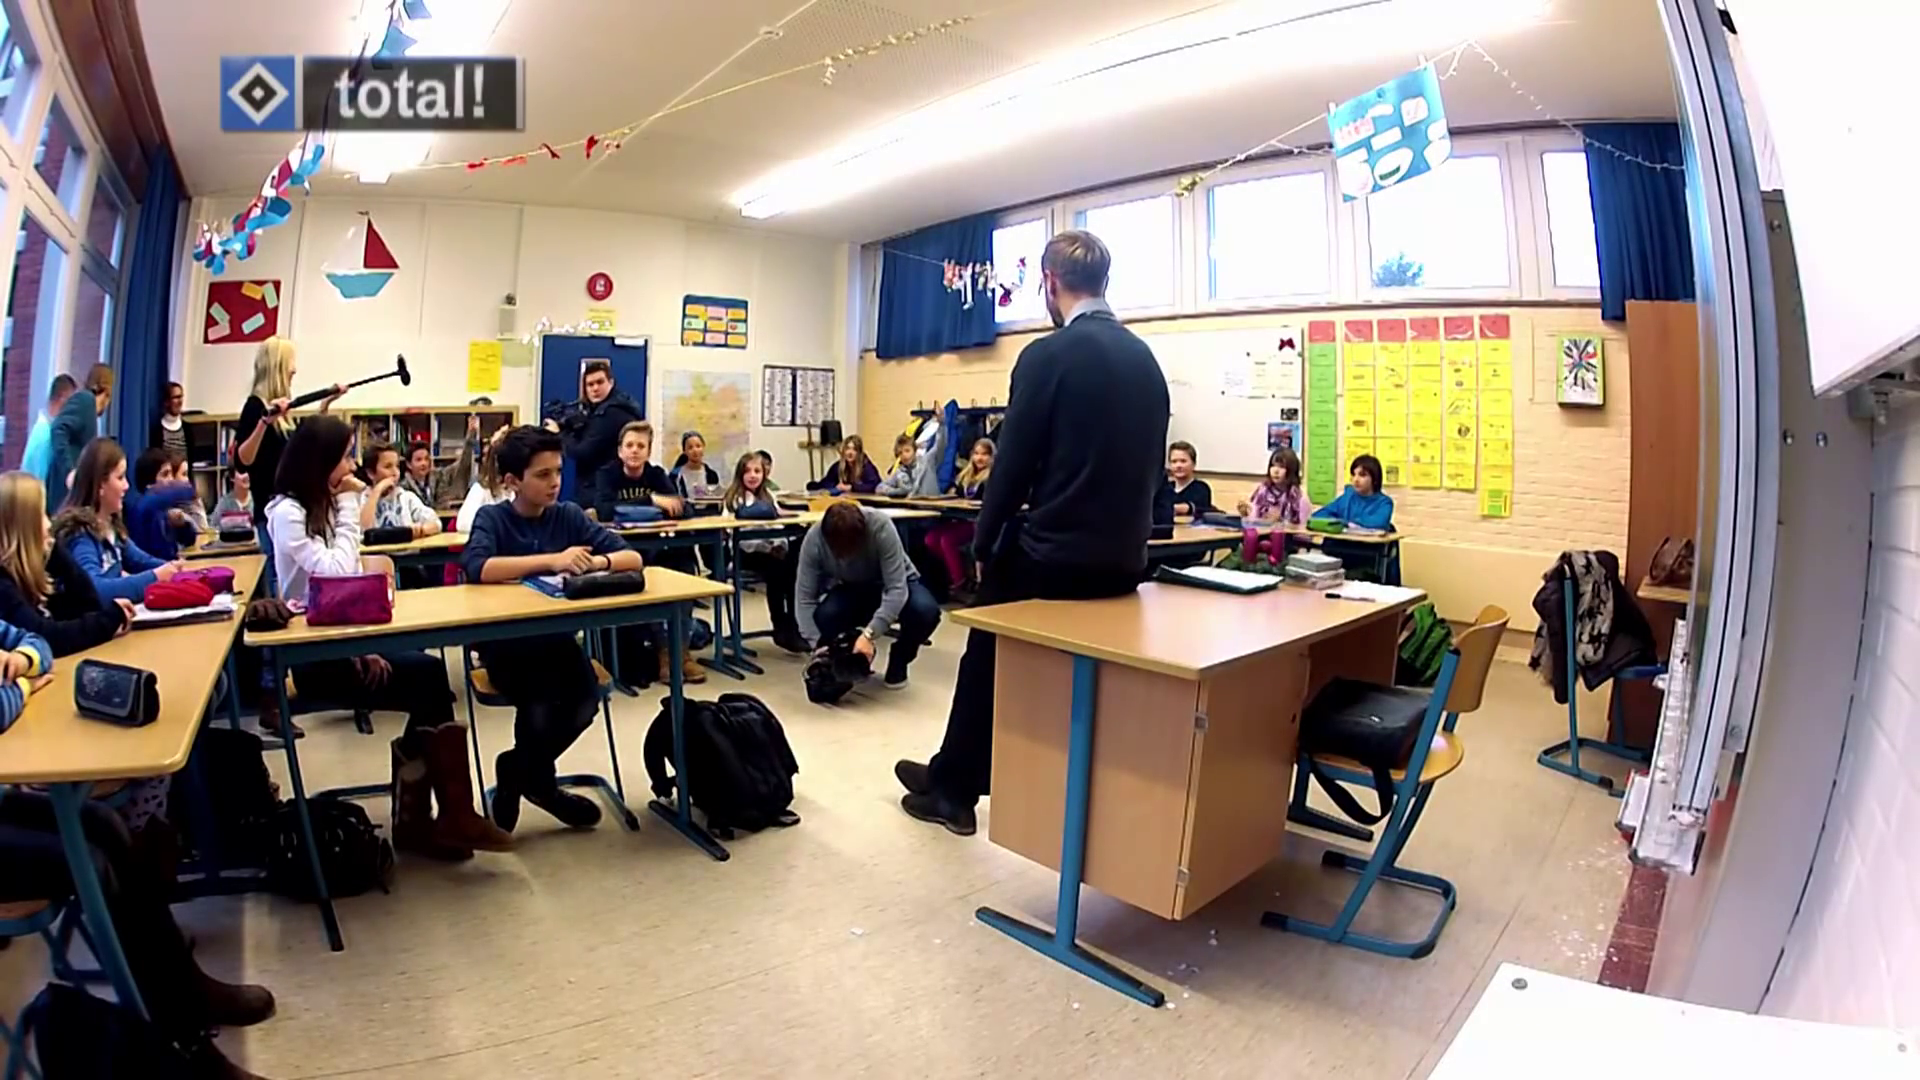
\includegraphics[width=0.8\linewidth]{img/Schulklasse}
	\caption{Eine Screenshot des YouTube-Videos \glqq Maxi Beister als Herr Müller überrascht eine Schulklasse\grqq \cite{Schulklasse_Video}}
	\label{fig:schulklasse}
\end{figure}

%\section{Verwendete Eingabegeräte \& Bibliotheken}
\label{hardware}
 wurden verschiedenen Farbkameras eingesetzt.\\
\\
%\subsection{Auswirkung von Pixelrauschen}
%Durch Aufnahme eines Schwarzbildes der Actioncam zeigt sich, dass das Pixelrauschen recht hoch ist, siehe \autoref{img_noishight}. Das Rauschen hat keine Normalverteilung, sondern es besteht aus kleinen Bereiche, die den selben fehlerhaften Farbwert besitzen.
%\begin{figure}
%	\centering
%	\fbox{
\includegraphics[width=1\linewidth]{img/NoisHight}}
%	\caption{Aufnahme eines Schwarz-Bildes $(2688\times 1520)$ der Actioncam um den Faktor 7 verstärkt und invertiert.}
%	\label{img_noishight}
%\end{figure}
Für die Umsetzung wurden Open Source Computer Vision (OpenCV 3.1) verwendet. Dies ist eine C/C++ Bibliothek von Algorithmen zur Bildverarbeitung in Echtzeit, veröffentlicht unter der BSD Lizenz (Berkeley
Software Distribution)\\
\cite{OpenCv_What_Is}\cite{wiki_Wha_is_OPenCV}
\cleardoublepage

\chapter{Evaluation}
Zuerst werden die einzelnen verwendeten Verfahren getestet bezüglich ihrer Stabilität bei sinkendem Informationsgehalt der Eingabe. Dazu wurden die einzelnen Verfahren auf verschieden skalierten Datensätzen getestet um anschließend ihre Verwendbarkeit unter realen Bedingungen getestet.
\section{OpenFace im Test}
Da mit diesem Verfahren die Landmarks bestimmt werden, aus denen die Gesichtsorientierung abgeleitet wird, sollen die Grenzen dieses Verfahrens ermittelt werden. Von Interesse ist die Bildqualität in der ein Gesicht dargestellt werden muss um dieses noch verarbeiten zu können und wie sehr diese Person von der Kamera abgewandt sein kann.\\
Das Herunterskalieren von Bildern ist nicht das selbe wie eine Aufnahme auf großer Distanz, ist aber ähnlich genug um eine Aussage darüber treffen zu können.\\
Zur Messung wurde der Datensatz von Labeled Faces in the Wild LFW \cite{database_Face} und BIWI Random Forests for Real Time 3D Face Analysis \cite{database_Face_Ori} verwendet.\\
Der LFW Bilddatensatz enthält Abbildungen verschiedener Personen mit einer durchschnittlichen Abbildung der Breite des Kopf von 95 Pixeln. Bei BIWI beträgt die durchschnittliche Breite 78 Pixel und die durchschnittliche Distanz zwischen Kamera und Proband beträgt etwa $95cm$.
\subsection{Auswirkung der Auflösung auf die Detektionsrate}
Durch die Aufgabenstellung muss das Verfahren zuverlässig bezüglich der Distanzen bzw. Darstellungsgröße sein.\\
Bei BIWIk wurde eine Selektion durchgeführt, da die Detektionsrate nur bei $63,4\%$ liegt und durch die Darstellung die Veränderung des Verlauf nur schwer zu erkennen ist.\\
Um die Grenzen der Methode auszuloten wurde das Bild mit unterschiedlichen Faktoren linear skaliert, um so weiter entferntere Gesichter zu simulieren.\\
Um die Detektionsrate zu bestimmen, wurde der Image-Detector von OpenFace auf den skalierten Bildern angewendet und gezählt wie oft der Detektor ein Gesicht erkannt hat. Dabei wurde nicht geprüft ob es sich dabei um ein korrektes Gesicht handelt.\\
Das Ergebnis dieser Messung ist in \autoref{img_lineareverkleinerung} dargestellt. Es ist zu erkennen, dass die Wahrscheinlichkeit einer erfolgreichen Detektion ab einer Skalierung von $0,64$ bei BIWI (Gesichter mit etwa 50 Pixel Breite) und $0,46$ bei LFW (Gesichter mit 44 Pixel Breite) rapide abnimmt. Bei der in \autoref{Versuch_1} beschriebenen Kamera entspricht dies einer Distanz von etwa $4,5m$.\\
\begin{figure}[p]
	\centering
	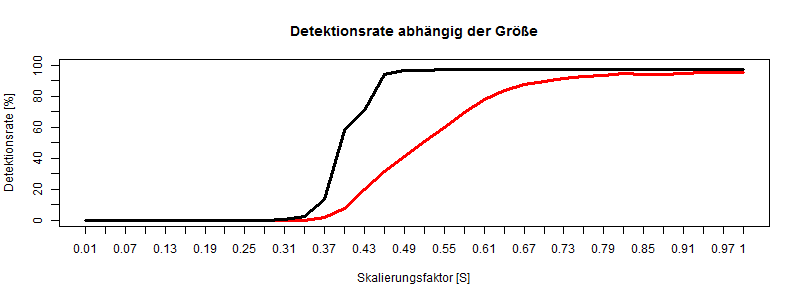
\includegraphics[width=\linewidth]{img_Skalierung/Gesicht_Rate}
	\caption{LFW \cite{database_Face} (schwarz) und BIWI \cite{database_Face_Ori} (rot) um den Skalierungsfaktor verkleinert und gegen die Erkennungsrate aufgetragen}
	\label{img_lineareverkleinerung}
\end{figure}
\subsection{Auswirkung von verschiedenen Skalierungesverfahren auf die Detektion}
\label{OpenFace_skal}
Um die Auswirkung der Skalierungsverfahren zu bestimmen, wurden verschiedene Gesichtsgrößen simuliert, indem alle Bilder von BIWI unf LFW um den angegeben Faktor linear verkleinert wurden und mit den angegebenen Verfahren wieder auf die Originalgröße gebracht.\\
Die Auswirkung der verschiedenen Skalierungsverfahren (Bicubic, Lanczos, Linear, Nearest-Neighbor) auf die Detektionsrate ist in \autoref{img_hochskalliern} dargestellt.\\
Es ist zu erkennen, dass die Detektionsrate über einen weiten Bereich, $[1;0,3]$ bei der Skalierung, nur sehr wenig abnimmt. Durch die Vergrößerung können somit jene Gesichter in Skalierungsbereichen ausgewertet werden, die ohne nicht erkennbar sind.\\
Erst bei den sehr kleinen Skalierungen ist ein wirklicher Unterschied zwischen den Verfahren zu erkennen. So nimmt die Detektionsrate bei  Nearest-Neighbor (rot) deutlich früher (BIWI $0,34/27$Pixel und LFW $0,22/21$Pixel) ab, als bei den anderen Verfahren (BIWI $0,22/17$Pixel und $0,13/12$Pixel). Das Bicubic (blau) und Lanczos (grün) Verfahren haben die höchste Detektionsrate und fallen zuletzt ab, wobei Bicubic minimal besser ausfällt.
\begin{figure}[p]
	\centering
	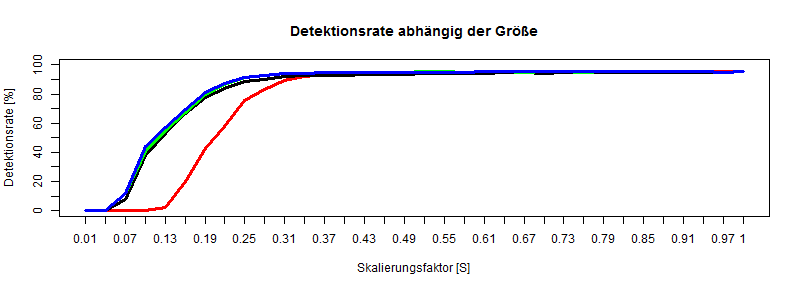
\includegraphics[width=\linewidth]{img_Skalierung/Resize_Rate_Ges}\\
	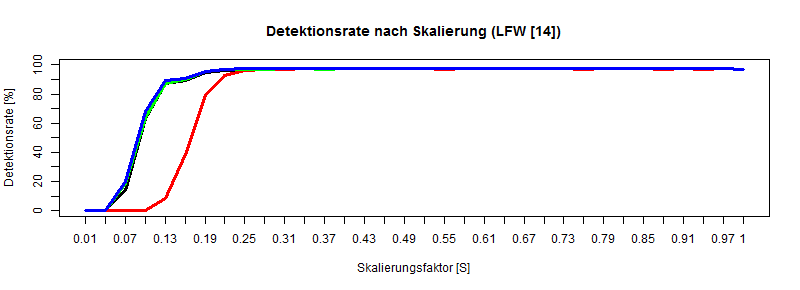
\includegraphics[width=\linewidth]{img_Skalierung/Resize_Rate_lfw}
	\caption{Bilder um den Skalierungsfaktor verkleinert und mit verschiedenen Verfahren wieder vergrößert.\\
		Bicubic (blau), Lanczos (grün), Linear (schwarz), N.-Neighbor (rot)}
	\label{img_hochskalliern}
\end{figure}
\subsection{Auswirkung von verschiedenen Skalierungesverfahren auf den Arbeitsbereich bezüglich Rotation}
In \autoref{img_Rot_Dif} ist der Median der Differenz zwischen per OpenFace berechnetem und im Datensatz angegebenem Kopforientierungswinkel aufgetragen.\\
Bei der X-Rotation zeigt sich, dass das Bicubic-Verfahren im Vergleich zu den anderen Verfahren etwa 2 Grad mehr abweicht, ein recht hoher Wert, zumal der Fehler von Lanczos, Linear und Nearest-Neighbor bei etwa $5,8^\circ$ bis zu einer Skalierung von $0,25$ liegt.\\
Der Median der Fehler auf der Y-Achse (nicken) bleibt ebenfalls gering mit $4,2^\circ$ vom Bicubic-Verfahren. Dabei liefern die anderen drei Verfahren nahezu identische Ergebnisse mit etwa $5^\circ$. Die jeweilige Qualität bleibt nahezu konstant bezüglich der Skalierung.\\
Die Z-Rotation wird am besten bestimmt mit einer Abweichung von etwa $2^\circ$ von allen getesteten Verfahren. Dabei ist aber auch zu beachten, das dieser Wertebereich im Datensatz deutlich geringer ausfällt, als bei den anderen beiden Rotationen.\\
Für alle Berechnungen zeigt sich, das der Fehler konstant bleibt, bis zu der Skalierung von $0.25$, bei der auch die Detektionsrate deutlich abfällt.\\
Neben der Qualität der bestimmten Winkel, ist auch der Arbeitsbereich von Interesse in dem Gesichter bei verschiedenen Skalierungen noch erkannt werden können. Ein Gesicht das außerhalb dieses Bereiches liegt kann nicht erkannt und ausgewertet werden.\\
In \autoref{img_Rot_Max} sind die Quantile bei $50\%; 80\%; 99\%$ und der Maximalwert, von den Rotationswinkel der Bilder aus BIWI \cite{database_Face_Ori} dargestellt, in denen ein Gesicht erkannt wurde. Durch den großen Unterschied zwischen dem $80\%$-Wert, $99\%$-Wert und dem Maximalwert liegt die Vermutung nahe, dass es sich bei diesen Werten um falsch detektierte Bilder handelt Dennoch kann eine Rotation des Kopfes von $45\%$ in alle Richtungen erkannt und ausgewertet werden.\\
Eine genaue Darstellung der Messung ist in \autoref{Abbildungen} abgebildet, für die X-Rotation \autoref{img_X_Rot_Skal}, Y-Rotation \autoref{img_Y_Rot_Skal} und Z-Rotation \autoref{img_Z_Rot_Skal}.
\begin{figure}
	\centering
	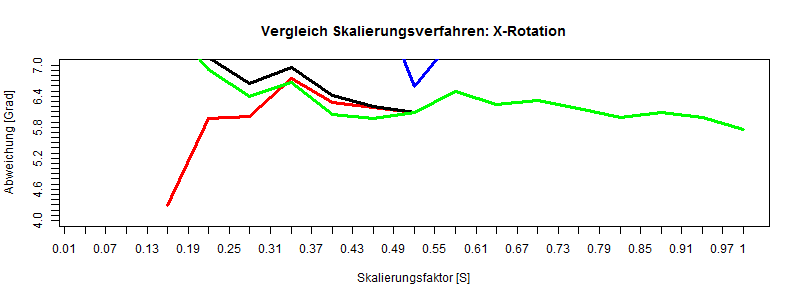
\includegraphics[width=\linewidth]{img_Skalierung/Skal_Diff_RX}
	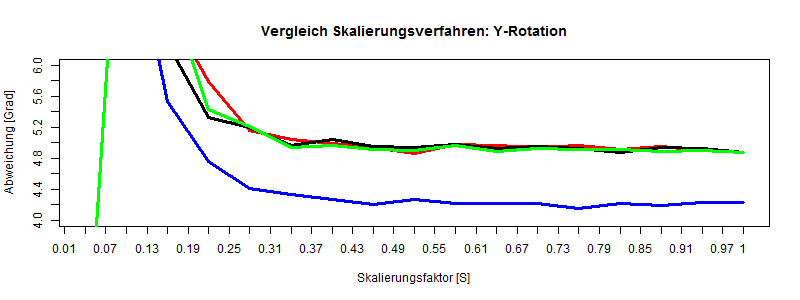
\includegraphics[width=\linewidth]{img_Skalierung/Skal_Diff_RY}
	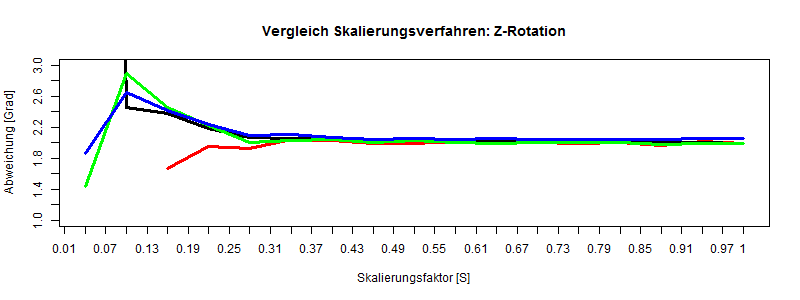
\includegraphics[width=\linewidth]{img_Skalierung/Skal_Diff_RZ}
	\caption{Dargestellt ist der Median der Abweichung zwischen der berechneten Drehung und der im Datensatzes.\\
		Bicubic (blau), Lanczos (grün), Linear (schwarz), N.-Neighbor (rot)}
	\label{img_Rot_Dif}
\end{figure}
\subsection{Auswirkung der Skalierungsverfahren auf die Positionsbestimmung}
Für eine zuverlässige Auswertung ist auch die Bestimmung der Position von Interesse. Zur Berechnung der Position auf BIWI wurde eine Brennweite der Kinekt-Kamera auf $531,15$ geschätzt, da es keine Angabe für den Datensatz gab.\\
Der Median der Differenz zwischen Datensatz und Rechnung ist in \autoref{img_Pos_Dif} dargestellt. Bei sehr kleinen Skalierungen existieren durchaus auch sehr große Fehler, diese wurden allerdings bei der Darstellung abgeschnitten, da bei dieser Größe die Detektionsrate so klein ist, dass die Ergebnisse nahezu irrelevant werden.\\
Aus der Abbildung ist zu entnehmen, dass die Position in horizontaler und vertikaler Richtung auf etwa $2,5cm$ genau bestimmt werden kann, die Distanz (Tiefe) auf etwa $2,8cm$ genau. Dies ist selbst bei sehr klein skalierten Bildern möglich.\\
Nearest-Neighbor hat bei der Berechnung der X-Position die geringste Abweichung zu den anderen getesteten Verfahren mit einem unterschied von etwa $1mm$.\\
Bei der Bestimmung der Y-Position hingegen, ist der Unterschied zwischen den vier Verfahren minimal.
\newpage
Die Differenz beträgt weniger als $1mm$ und keines der Verfahren zeigt einen aussagekräftigen Unterschied zu den anderen.\\
Eine ausführliche Darstellung der Messung ist in \autoref{img_X_Pos_Skal}, \autoref{img_Y_Pos_Skal} und \autoref{img_Z_Pos_Skal} dargestellt.
\begin{figure}
	\centering
	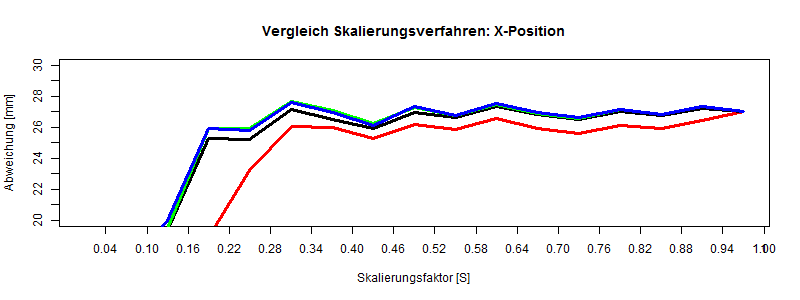
\includegraphics[width=\linewidth]{img_Skalierung/Skal_Diff_TX}
	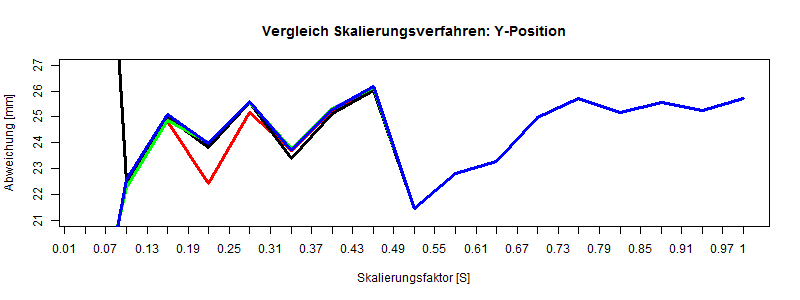
\includegraphics[width=\linewidth]{img_Skalierung/Skal_Diff_TY}
	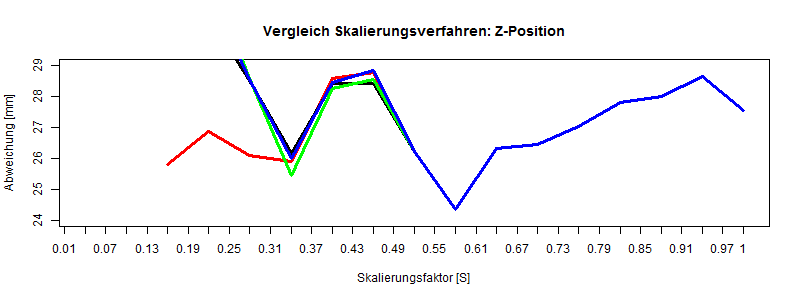
\includegraphics[width=\linewidth]{img_Skalierung/Skal_Diff_TZ}
	\caption{Dargestellt ist der Median der Abweichung zwischen der berechneten Position und der im Datensatzes.\\
		Bicubic (blau), Lanczos (grün), Linear (schwarz), N.-Neighbor (rot)}
	\label{img_Pos_Dif}
\end{figure}
\subsection{Auswirkung von Pixelrauschen auf die Detektion}
Mit diesem Test soll geprüft werden, welches der Verfahren auch stabil gegenüber Rauschen ist um einen besseren Eindruck für die Verwendbarkeit bei realen Aufnahmen zu erhalten.\\
Das Rauschen wird simuliert, indem für jedes Pixel eine Wahrscheinlichkeit von $50\%$ besteht auf eine gleichverteilte Abweichung von $\pm 10\%$ des originalen Farbwertes. Die Bilder von LFW \cite{database_Face} wurden entsprechend verkleinert, mit Rauschen versehen um sie anschließend mit den unterschiedlichen Verfahren zu vergrößern. Dieser Vorgang wurde für jedes Bild viermal wiederholt um Zufälligkeiten bei der Rauschsimulation zu vermeiden.\\
Wie zu erwarten ist Nearest-Neighbor am schlechtesten, aber auch zwischen den anderen Verfahren sind nun Unterschiede zu erkennen, siehe \autoref{img_hochskalliern_nois}. Die gesamte Erkennungsrate ist deutlich kleiner als ohne Rauschen, wobei der Skalierunfsfaktor von $0.22$, ab welcher die Erkennungsrate rapide abfällt, beibehalten wird.
\begin{figure}
	\centering
	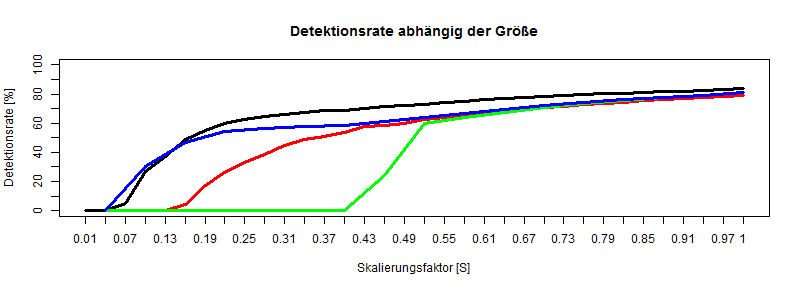
\includegraphics[width=\linewidth]{img_Skalierung/Hochskalliern_Nois}
	\caption{Detektionsrate auf Bilder von Labeled Faces in the Wild \cite{database_Face} mit Pixelrauschen ($50\%$ Wahrscheinlichkeit auf $10\%$ Abweichung)\\Bicubic (blau), Lanczos (grün), Linear (schwarz), N.-Neighbor (rot)}
	\label{img_hochskalliern_nois}
\end{figure}
\subsection{Auswirkung der verschiedenen Rechenverfahren für die Position}
Um die Qualität der Berechnung auf verschiedenen Distanzen zu ermitteln, wurde der BIWI Datensatz \cite{database_Face_Ori} verwendet, da für jedes Gesicht die Position und Orientierung bekannt ist.
Die durchschnittliche Distanz zwischen Kamera und Kopf beträgt ca $70cm$ bei einer Kopfbreite von 78 Pixel. Um die verschiedenen Distanzen zwischen Probanden und Kamera zu simulieren, wurden die Bilder mit dem angegebene Skalierungsfaktor (X-Achse) linear verkleinert.\\
Da verschiedene Verfahren zur Bestimmung der Position und Orientierung zur Verfügung stehen, sollen diese miteinander verglichen werden. Zur Bestimmung wurde nur das RGB-Bild verwendet und nicht zusätzlich die Tiefenaufnahme, da diese in der Anwendung auch nicht vorhanden ist.
\subsubsection{Position}
Zur Bestimmung der Position gibt es zwei Verfahren, die direkte mittels Brennweite und Skalierung oder Überführungsmatrix von 3D zu 2D Landmarks arbeiten.\\
Die Funktionen PoseCamera und PoseWorld verwenden die einfache Bestimmung mittels Skalierung und CorrectPoseCamera und CorrectPoseWorld die Überführung von 3D und 2D Landmarks, daher überlagern sich die Linien in \autoref{img_Verfahren_Pos}, da die jeweiligen Verfahren nach dem selben Prinzip rechnen.\\
Der schnelle Abfall der Genauigkeit bei der Skalierung $0,25$ ist an der selben Stelle an der auch die Detektionsrate stark absinkt, siehe \autoref{OpenFace_skal}. Somit kann das Verfahren bis zu seiner Grenze eingesetzt werden und erst, wenn die Detektion schwierig wird steigt auch der Fehler.
\begin{figure}
	\centering
	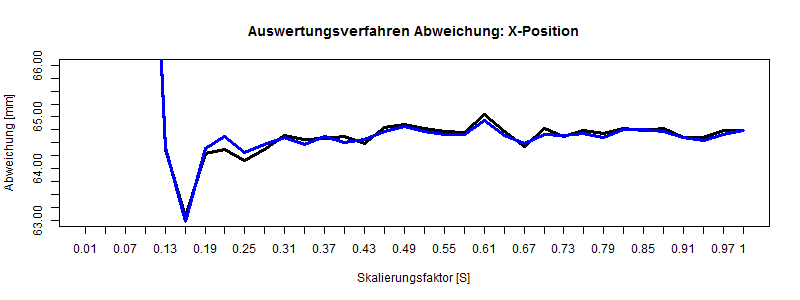
\includegraphics[width=\linewidth]{img_Skalierung/Verfahren_TX}
	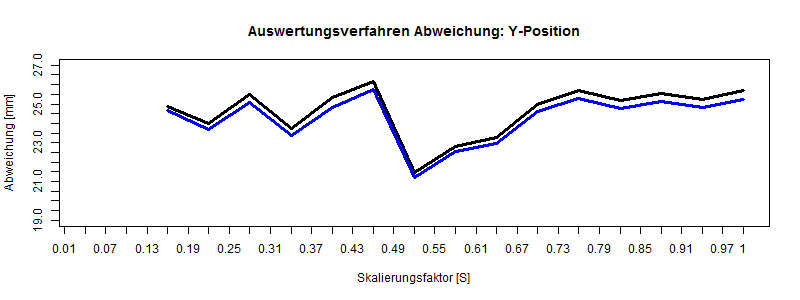
\includegraphics[width=\linewidth]{img_Skalierung/Verfahren_TY}
	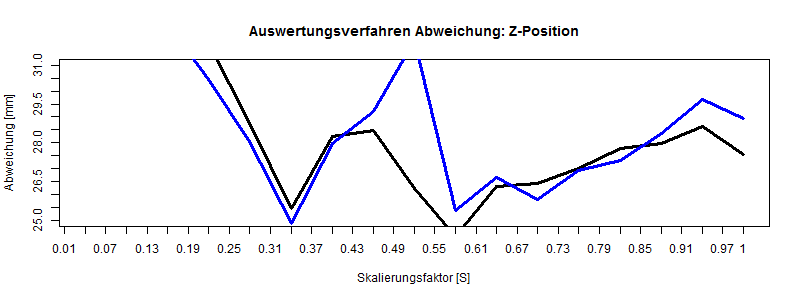
\includegraphics[width=\linewidth]{img_Skalierung/Verfahren_TZ}
	\caption{Dargestellt ist der Median der Abweichung in Millimeter der Positionsbestimmung auf Bilder die mit Lanczos skaliert wurden.\\
	PoseWorld (schwarz), PoseCamera (rot, verdeckt von PW), CorrectPoseCamera (grün, verdeckt von CPW) und CorrectPoseWorld (blau)\\
	Oben: X-Position, Mitte: Y-Position, Unten: Z-Position}
	\label{img_Verfahren_Pos}
\end{figure}
\subsubsection{Orientierung}
Bei der Rotation zeigen sich nun Unterschiede zwischen den einzelnen Verfahren, da bei PoseWorld und CorrectPoseWorld auch die Position im Kamerabild berücksichtigt wird.\\
Aus \autoref{img_Verfahren_Rot} ist zu entnehmen, dass die zusätzliche Korrektur das Ergebnis weiter verbessert wird, wenn die Pixelorientierungen mit beachtet werden.
\begin{figure}
	\centering
	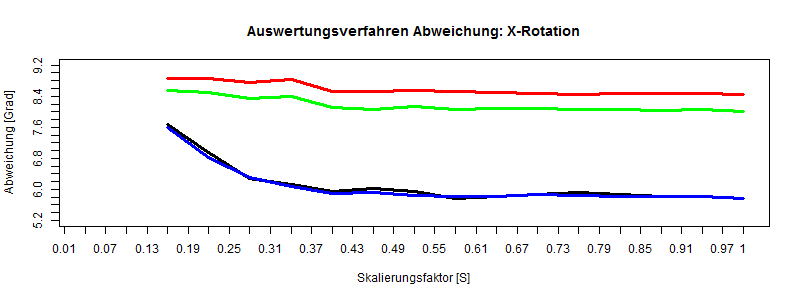
\includegraphics[width=\linewidth]{img_Skalierung/Verfahren_RX}
	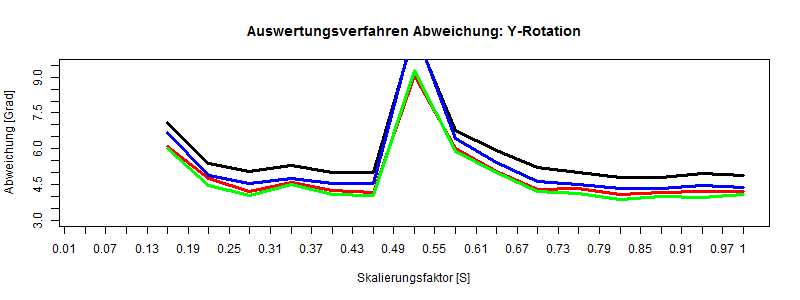
\includegraphics[width=\linewidth]{img_Skalierung/Verfahren_RY}
	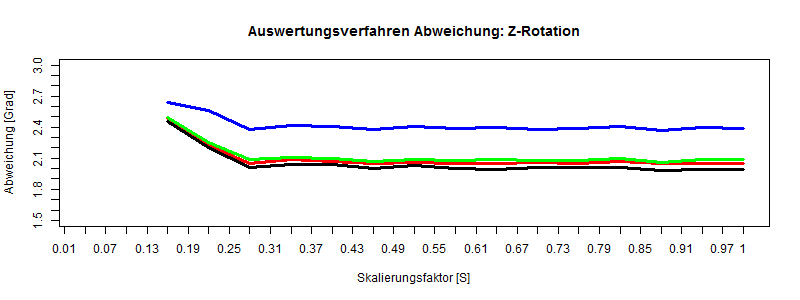
\includegraphics[width=\linewidth]{img_Skalierung/Verfahren_RZ}
	\caption{Dargestellt ist der Median der Abweichung in Grad der Positionsbestimmung auf Bilder die mit Lanczos skaliert wurden.\\
		PoseWorld (schwarz), PoseCamera (rot), CorrectPoseCamera (grün) und CorrectPoseWorld (blau)\\
		Oben: X-Rotation, Mitte: Y-Rotation, Unten: Z-Rotation}
	\label{img_Verfahren_Rot}
\end{figure}
\subsubsection{Ergebnis}
Es zeigt sich, dass CorrectPoseWorld, also die komplexe Bestimmung der Position mittels 2D/3D Landmarks und zusätzlicher Korrektur der Winkel die besten Ergebnisse liefert im Test.\\
Im Test ist die Überführung von 3D zu 2D Landmarks am besten (CorrectPoseCamera und CorrectPoseWorld) kann sich allerdings auch ändern wenn die Kamera Parameter besser abgeschätzt sind, da ohne eine Tiefenaufnahme die korrekte Überführung nur geschätzt werden kann und sich Fehler fortpflanzen können.
\subsection{Ergebnis bezüglich Verwendbarkeit}
Anhand der Detektionsrate abhängig von der Skalierung, siehe \autoref{img_lineareverkleinerung}, kann entnommen werden, dass Gesichter unter 50 Pixel Größe nicht mehr sinnvoll erkannt werden können. Somit ergibt sich eine maximale Distanz von etwa $4,5m$ (basierend auf der Actioncam) für eine Analyse.\\
Da die maximale Distanz, auf der gearbeitet werden soll, jedoch $(8m)$ beträgt, ergibt sich eine Gesichtsgröße von etwa 22 Pixel. Dies entspricht einer Skalierung von $0,28$ für den BIWI-Datensatz. Bei dieser Bildgröße ist in der Standardanwendung ohne Skalierung keine Detektion möglich.\\
Werden die Bildbereiche hingegen hochskaliert, zeigt der Test, dass sogar Gesichter mit einer Größe von unter 22 Pixel (Skalierung $0,25$, $8m$) gefunden und analysiert werden können. Dies bedeutet, dass mit diesem Trick auch mit der Hälfte der Bildinformationen noch gearbeitet werden kann, wenn die Eingabe dadurch dem Trainingsdatensatz eher entspricht.\\
Für eine erfolgreiche Analyse sind die Parameter Detektionsrate, Qualität der Rotation und Qualität der Position relevant. Daher wurden die verschiedenen Skalierungsverfahren in diesen Parametern bei unterschiedlichen Größen der Eingabebilder verglichen.\\
Die höchste Detektionsrate bei den Skalierungen erreicht Bicubic, wobei der Unterschied zu Lanczos und Linear so minimal ausfällt, das sie als Gleichwertig in diesem Bereich betrachtet werden kann. Es zeigt sich auch die deutliche Schwäche von Nearest-Neighbor, die Detektionsrate nimmt deutlich früher ab als bei den anderen.\\
Bei der Bestimmung der Rotation kann nur ein geringer Unterschied zwischen den einzelnen Verfahren erkannt werden. Für die X-Rotation hat das Bicubic-Verfahren einen um etwa $2^\circ$ größeren Fehler als die anderen, bei der Y-Rotation hingegen $0,8^\circ$ genauer ist. Bei der Z-Rotation ist kein klarer Unterschied zu erkennen, somit ist bei diesem Parameter die Wahl des Verfahrens egal.\\
Zur Bestimmung der Position ist das lineare Verfahren am besten geeignet, da es den kleinsten Fehler aufweist, wobei der Unterschied mit $1mm$ sehr gering ausfällt.\\
Der Test mit dem Pixelrauschen soll etwaige Bildfehler simulieren, wie es bei schlechten Kameras der Fall sein kann, was die Auswertung auf kleinen Bildausschnitten erschwert. Somit kann auch gezeigt werden, dass dieser Trick mit der Vergrößerung auch sehr wahrscheinlich in der späteren Anwendung funktionieren wird.
\newpage
In diesem Test erreicht das lineare Verfahren die höchste Detektionsrate, diesmal ist der Unterschied zwischen den einzelnen Verfahren deutlich besser erkennbar.\\
Somit erfüllt das lineare Verfahren die Parameter am besten, wobei der Unterschied zwischen den einzelnen recht gering ausfällt und die Wahl des Skalierungsverfahren von anderen Kriterien abhängig gemacht werden kann, wie z.B. von der Rechenzeit. Dabei kann vom Nearest-Neighbor abgeraten werden wegen dem deutlich früheren Abfall der Detektionsrate.\\
Theoretisch wären sogar Distanzen bis zu $14m$ ($12$Pixel) möglich, basierend auf der hohen Auflösung der Actioncam für eine erfolgreiche Detektion.\\
Der Unterschied bei Skalierung 1 (Originalgröße) zu der Ergebnissen in Paper \cite{OpenFace} kann an der Verwendung des Median anstelle des Durchschnitts als auch an der verwendung von verschiedenen Kameraparametern liegen.
\section{ElSe im Test}
Der Ursprüngliche ElSe-Algorithmus wurde für Eye-Tracking Brillen entwickelt, also für ein qualitativ hochwertiges Bild eines Auges, daher soll geprüft werden in wieweit es in dieser Anwendung eingesetzt werden kann.\\
Um die einzelnen Grau-Verfahren besser vergleichen zu können, wurden künstliche Augen aus dem Datensatz \cite{database_Eye} verwendet damit die exakte Position der Landmarks bekannt ist.\\
Ein gutes Verfahren muss stabil gegenüber der Skalierung sein, damit es auch auf kleinen Bereichen zuverlässig arbeitet. Da für die spätere Anwendung vor allem das Zentrum der Pupille von Interesse ist, wird der euklidische Abstand zum Zentrum als Qualitätsmaß verwendet.\\
Da ElSe für Eye-Tracking Brillen entwickelt wurde ist der Augenbereich genauer bestimmt als im Datensatz enthalten, daher wurde der Bildbereich soweit verkleinert, dass nur noch alle Landmarks des Auges mit etwas Rand dargestellt werden, um diesen Anforderungen entsprechend nahe zu kommen.\\
Somit sind die Bildausschnitte im Datensatz auf denen gerechnet wird etwa 64 auf 29 Pixel groß und werden für die Verarbeitung auf eine Breite von 384 Pixeln vergrößert, die Auflösung, wofür ElSe entwickelt wurde. Da durch die Skalierung allerdings keine zusätzlichen Informationen entstehen, ist vor allem die grobe Bestimmung der Ellipse, beschrieben in \autoref{ElSe_Grob}, von Interesse. Diese Auswahl des Bildbereiches kann auch in der späteren Anwendung eingesetzt werden, da der Augenbereich durch eigene Landmarks in der Gesichtsanalyse, relativ genau bestimmt ist.\\
Um die Qualität der Berechnung bei verschiedenen Größen zu ermittelt, wurde das Bild linear verkleinert.
\subsection{Auswirkung des Filterradius}
Ein wichtiger Parameter des ElSe-Verfahrens ist der Radius des Filters. Um den besten Parameter zu bestimmen wurde der Augen-Datensatz \cite{database_Eye} verwendet und die Augenpartie ausgeschnitten. Im Datensatz besitzen die abgebildeten Augen durchschnittlich eine Pupille mit 15 Pixel und eine Iris von 34 Pixel Durchmesser.\\
In \autoref{img_vergleich_PI} ist zu erkennen, dass der Radius signifikant für die Qualität der Berechnung ist. Da für die spätere Anwendung vor allem das Zentrum der Pupille von Interesse ist, vgl. \autoref{OpenFace_Blickrichtung}, muss ElSe in diesem Aspekt zuverlässig Ergebnisse liefern.\\
Im Versuch hat sich ein Radius von etwa einem Zwölftel des zu erwartenden Durchmessers der Iris bzw. Pupille als sinnvoll erwiesen, um deren Ausmaße möglichst exakt zu bestimmen. Im Versuch entspricht dies 8 und 18 Pixel.\\
Um die Position des Zentrums der Iris und der Pupille möglichst gut zu bestimmen, erwies sich ein Radius von 10 Pixel am besten, siehe \autoref{img_vergleich_A}, wobei dieser Fehler nicht so sehr steigt bei Veränderung des Radius, als bei der Größenbestimmung von Pupille und Iris.
\begin{figure}
	\centering
	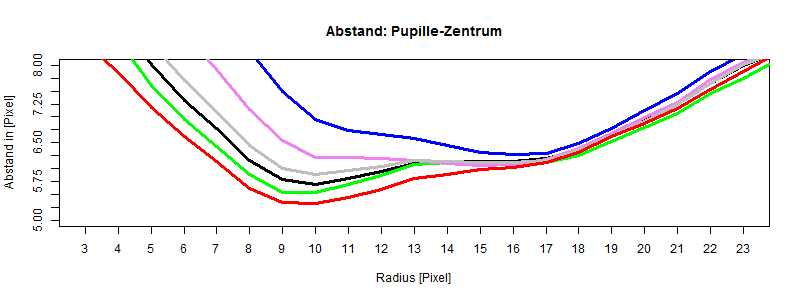
\includegraphics[width=\linewidth]{Eye_Img_Box/Vergleich_A}
	\caption{Median-Abstand in Pixel des Zentrums der Pupille gegen die Veränderung des Radius des Filters.\\
		Verfahren: Gleam (rot), Luminance (schwarz), Max (grün), Min (violett), New-Gleam (grau), Quadrat (blau)}
	\label{img_vergleich_A}
\end{figure}
\begin{figure}
	\centering
	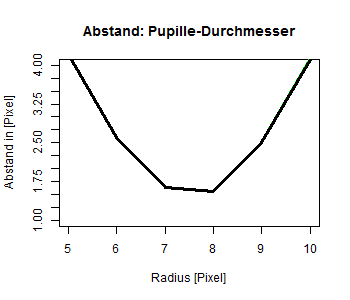
\includegraphics[width=0.49\linewidth]{Eye_Img_Box/Vergleich_P}
	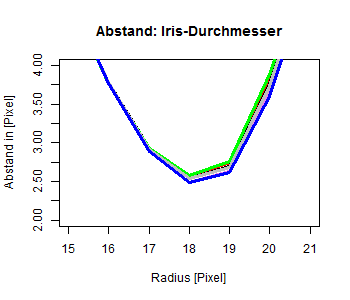
\includegraphics[width=0.49\linewidth]{Eye_Img_Box/Vergleich_I}
	\caption{Differenz zwischen den Radien gegen die Veränderung des Radius des Filters von Pupille (links) und Iris (rechts)\\
		Verfahren: Gleam (rot), Luminance (schwarz), Max (grün), Min (violett), New-Gleam (grau), Quadrat (blau)}
	\label{img_vergleich_PI}
\end{figure}
\subsection{Auswirkung der verschiedenen Graubild-Verfahren}
\label{grau_Auswirkung_ElSe}
Es zeigt sich, dass die Verfahren mit denen der Farbwert in einen Grauwert überführt wird, durchaus Auswirkungen auf die Qualität der Berechnung haben.\\
Für die Bewertung der Verfahren werden folgende Kriterien verwendet: Die Differenz zwischen den berechneten und tatsächlichen Radien von Pupille und Iris sowie die Abweichung des berechneten Zentrums der Pupille.\\
Der minimale Abstand der berechneten Zentren ergibt sich bei dem Gleam-Verfahren mit $5.327$ Pixel als Median, siehe \autoref{img_vergleich_A}. Der beste Radius für den Filter ist für die Position der Iris bei 10 Pixel.\\
Ein Unterschied zwischen den Verfahren konnte bei der Bestimmung des Radius der Pupille nicht gefunden werden, siehe \autoref{img_vergleich_PI} links. Der beste Radius für den Filter ist im Test bei 8 Pixel und ergibt eine Abweichung von $1,555$ Pixel.\\
Für die Bestimmung der Iris hat das quadratische Verfahren die geringste mittlere Abweichung mit $2,488$ Pixel, nur etwas genauer als Min-Verfahren ($2,49$ Pixel). Für diese Berechnung ist ein Radius des Filters von 18 Pixel am besten gewählt.\\
Somit wurden drei Verfahren ausgewählt um diese näher zu untersuchen, Gleam mit der geringsten Abweichung des Zentrums, Quadrat als bestes Resultat bei der Iris und Luminance da es ein Standartverfahren ist. Mit allen Verfahren wurde die Berechnung zur Pupille/Zentrum/Iris für verschieden groß skalierte Bilder bestimmt mit ihren jeweiligen optimalen Filterradien.\\
Bei der Berechnung der Pupille auf den unterschiedlich großen Abbildungen ist weiterhin kein Unterschied zu erkennen, siehe \autoref{img_Vergleich_Scal_PI} oben.\\
Auch bleiben die Unterschiede der Verfahren erhalten und die Fehler auf dem glichen Niveau bis zu einer Skalierung von $0,15$, ab welcher die Berechnung bei allen Verfahren scheitert. So liefert das Gleam-Verfahren die besten Ergebnisse im Bezug auf das Zentrum, wo hingegen das Quatrat-Verfahren geeignet für die Bestimmung des Iris-Radius ist.
\begin{figure}
	\centering
	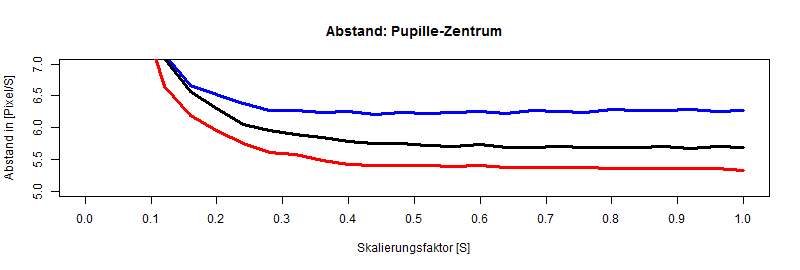
\includegraphics[width=\linewidth]{Eye_Img_Box/Vergleich_Scal_A}
	\caption{Euklidischer Abstand in Pixel zwischen dem berechneten Zentrum der Pupille und dem des Datensatzes gegen die Veränderung des Radius des Filters.\\
		Verfahren: Gleam (rot), Luminance (schwarz),  Quadrat (blau)}
	\label{img_Vergleich_Scal_A}
\end{figure}
\begin{figure}
	\centering
	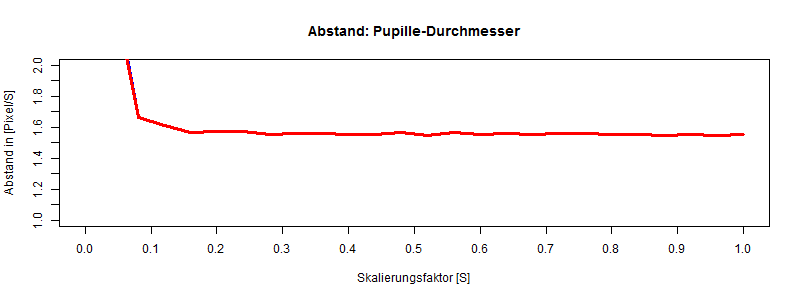
\includegraphics[width=\linewidth]{Eye_Img_Box/Vergleich_Scal_P}
	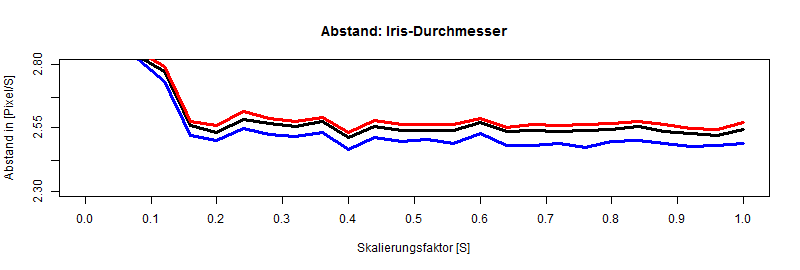
\includegraphics[width=\linewidth]{Eye_Img_Box/Vergleich_Scal_I}
	\caption{Differenz in Pixel zwischen den Radien der Berechnung und dem des Datensatzes gegen die Veränderung des Radius des Filters.\\ Oben: Pupille mit Filterradius 8, Unten: Iris mit Filterradius 18\\
		Verfahren: Gleam (rot), Luminance (schwarz), Quadrat (blau)}
	\label{img_Vergleich_Scal_PI}
\end{figure}
\subsection{Vergleich zu OpenFace}
Als Referenz wird das Ergebnis von OpenFace, für die zusätzlich bestimmten Landmarks der Augen, verwendet. Dies wurde auch auf dem Augendatensatz \cite{database_Eye} angewendet, um vergleichbare Ergebnisse zu erhalten.\\
Wird \autoref{OpenFace_Eye} mit \autoref{img_Vergleich_Scal_A} bzw. \autoref{ElSe_scall} verglichen so ist zu erkennen, das OpenFace im Mittel einen geringen Fehler bis zu einer Skalierung von $0,47$ besitzt als ElSe. Ab diesem Wert hat ElSe einen geringen mittleren Fehler, da die Abweichung fast unverändert bis $0,12$ beibehalten wird.\\
Da diese Qualität von ElSe nur erreicht werden kann, wenn es auf einem passenden Bildausschnitt angewendet wird, ist auch die Detektion des Auges von Interesse.\\
Aus \autoref{OpenFace_Eye_Box} ist zu entnehmen, dass der Bereich des Auges zwar nicht so exakt bestimmt wird, allerdings überdeckt er den relevanten Bereich ausreichend genau damit die Landmarks im Bildausschnitt liegen. Somit kann dieser Bildausschnitt als Eingabe von ElSe verwendet werden.
\begin{figure}
	\centering
	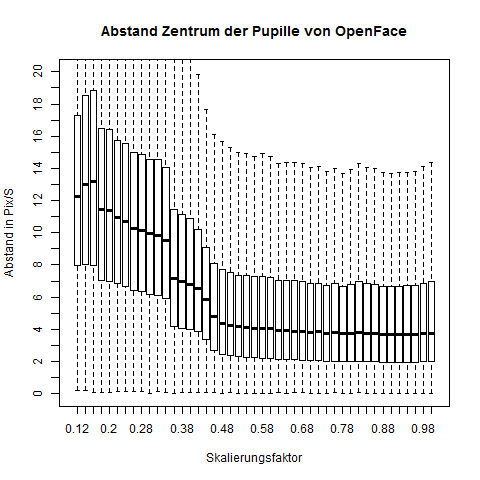
\includegraphics[width=0.49\linewidth]{Eye_Img_Box/Openface_PC}
	\includegraphics[width=0.49\linewidth]{Eye_Img_Box/Openface_PW}
	%\includegraphics[width=0.45\linewidth]{Eye_Img/OpenFace_Zentrum_P}
	%\includegraphics[width=0.45\linewidth]{Eye_Img/OpenFace_Width_P}
	\caption{Auswirkung der Bildgröße auf die Qualität der Augendetektion von OpenFace. Aufgetragen ist die Abweichung [Pixel/Skalierung] gegen den Skalierungsfaktor.}
	\label{OpenFace_Eye}
\end{figure}
\subsection{Ergebnis}
Die Tests haben ergeben, das ElSe mit einem Radius von 10 Pixel auf Bildern die mithilfe von Gleam ins Graue überführt wurde die besten Ergebnisse liefert. Dabei ist das Verfahren stabil gegenüber der Skalierung und kann die Iris bis zu einer Größe von 3 Pixel erkennen, das einer Distanz von etwa $4m$ entspricht (Basierend auf der Actioncam).\\
Allerdings hat der Vergleich ergeben, das bis zu einer Skalierung von $0,47$ ElSe schlechtere Ergebnisse liefert als das OpenFace-Augen-CNN.\\
So kann das Ergebnis von OpenFace bei Bilder in denen die Iris größer als 21 Pixel ist direkt als Lösung verwendet werden, da der mögliche Fehler von OpenFace geringer ist als der von ElSe.\\
Im Bereich zwischen 17 und 15 Pixel ($0,5-0,44$) können beide Ergebnisse kombiniert werden, da sie ungefähr gleich gute Ergebnisse liefern um den Gesamtfehler zu minimiren, da die beiden Verfahren unabhängig voneinander arbeiten.\\
Sollte die Iris im Originalbild noch kleiner sein, so ist ElSe deutlich genauer, da es noch bis zu einer Irisgröße von 3 Pixel stabil funktioniert.\\
Eine genauere Darstellung der Messergebnisse ist in \autoref{Abbildungen} dargestellt. Die Auswirkung der Radien und der verschieden Verfahren auf die Pupille ist in \autoref{ElSe_Gray_Pupille}, auf die Iris in \autoref{ElSe_Gray_Iris} und auf die Bestimmung des Zentrums in \autoref{ElSe_Gray_Zentrum} dargestellt, die Auswirkung der Skalierung in \autoref{ElSe_scall}.\\
Bei realen Aufnahmen sind Bildfehler unvermeidlich, so können Reflektionen (Brille, Kontaktlinse usw.), Make-Up und körperliche Eigenschaften wie Augenfarbe die Detektion erschweren. Ein Problem das schon im originalen Test \cite{ElSe} aufgetreten ist, wenn der Farbunterschied zwischen Iris und Pupille recht gering ausfällt oder durch Reflektionen der Kantenverlauf gestört wird, wodurch die maximale Distanz in der eine Auswertung der augen möglich ist weiter sinkt.
\subsection{Auswirkung der verschiedenen Rechenverfahren für die Position}
Um die Qualität der Berechnung auf verschiedenen Distanzen zu ermitteln, wurde der BIWI Datensatz \cite{database_Face_Ori} verwendet, da für jedes Gesicht die Position und Orientierung bekannt ist.
Die durchschnittliche Distanz zwischen Kamera und Kopf beträgt ca $70cm$ bei einer Kopfbreite von 78 Pixel. Um die verschiedenen Distanzen zwischen Probanden und Kamera zu simulieren, wurden die Bilder mit dem angegebene Skalierungsfaktor (X-Achse) linear verkleinert.\\
Da verschiedene Verfahren zur Bestimmung der Position und Orientierung zur Verfügung stehen, sollen diese miteinander verglichen werden. Zur Bestimmung wurde nur das RGB-Bild verwendet und nicht zusätzlich die Tiefenaufnahme, da diese in der Anwendung auch nicht vorhanden ist.
\subsubsection{Position}
Zur Bestimmung der Position gibt es zwei Verfahren, die direkte mittels Brennweite und Skalierung oder Überführungsmatrix von 3D zu 2D Landmarks arbeiten.\\
Die Funktionen PoseCamera und PoseWorld verwenden die einfache Bestimmung mittels Skalierung und CorrectPoseCamera und CorrectPoseWorld die Überführung von 3D und 2D Landmarks, daher überlagern sich die Linien in \autoref{img_Verfahren_Pos}, da die jeweiligen Verfahren nach dem selben Prinzip rechnen.\\
Der schnelle Abfall der Genauigkeit bei der Skalierung $0,25$ ist an der selben Stelle an der auch die Detektionsrate stark absinkt, siehe \autoref{OpenFace_skal}. Somit kann das Verfahren bis zu seiner Grenze eingesetzt werden und erst, wenn die Detektion schwierig wird steigt auch der Fehler.
\begin{figure}
	\centering
	\includegraphics[width=\linewidth]{img_Skalierung/Verfahren_TX}
	\includegraphics[width=\linewidth]{img_Skalierung/Verfahren_TY}
	\includegraphics[width=\linewidth]{img_Skalierung/Verfahren_TZ}
	\caption{Dargestellt ist der Median der Abweichung in Millimeter der Positionsbestimmung auf Bilder die mit Lanczos skaliert wurden.\\
	PoseWorld (schwarz), PoseCamera (rot, verdeckt von PW), CorrectPoseCamera (grün, verdeckt von CPW) und CorrectPoseWorld (blau)\\
	Oben: X-Position, Mitte: Y-Position, Unten: Z-Position}
	\label{img_Verfahren_Pos}
\end{figure}
\subsubsection{Orientierung}
Bei der Rotation zeigen sich nun Unterschiede zwischen den einzelnen Verfahren, da bei PoseWorld und CorrectPoseWorld auch die Position im Kamerabild berücksichtigt wird.\\
Aus \autoref{img_Verfahren_Rot} ist zu entnehmen, dass die zusätzliche Korrektur das Ergebnis weiter verbessert wird, wenn die Pixelorientierungen mit beachtet werden.
\begin{figure}
	\centering
	\includegraphics[width=\linewidth]{img_Skalierung/Verfahren_RX}
	\includegraphics[width=\linewidth]{img_Skalierung/Verfahren_RY}
	\includegraphics[width=\linewidth]{img_Skalierung/Verfahren_RZ}
	\caption{Dargestellt ist der Median der Abweichung in Grad der Positionsbestimmung auf Bilder die mit Lanczos skaliert wurden.\\
		PoseWorld (schwarz), PoseCamera (rot), CorrectPoseCamera (grün) und CorrectPoseWorld (blau)\\
		Oben: X-Rotation, Mitte: Y-Rotation, Unten: Z-Rotation}
	\label{img_Verfahren_Rot}
\end{figure}
\subsubsection{Ergebnis}
Es zeigt sich, dass CorrectPoseWorld, also die komplexe Bestimmung der Position mittels 2D/3D Landmarks und zusätzlicher Korrektur der Winkel die besten Ergebnisse liefert im Test.\\
Im Test ist die Überführung von 3D zu 2D Landmarks am besten (CorrectPoseCamera und CorrectPoseWorld) kann sich allerdings auch ändern wenn die Kamera Parameter besser abgeschätzt sind, da ohne eine Tiefenaufnahme die korrekte Überführung nur geschätzt werden kann und sich Fehler fortpflanzen können.
\section{Versuch 1 - Arbeitsbereich der Verfahren}
\label{Versuch_1}
Mit diesem Versuch soll der Zusammenhang zwischen Standort eines Probanden und Position des Blickziels untersucht werden. Dazu wird eine Klassenzimmerumgebung simuliert, in der sowohl Standort als auch die Blickziele relativ zur Kamera bekannt sind.\\
Als Messinstrument für die Versuche 1 und 2 wurde die Explorer 4K Actioncam verwendet, da sie eine hohe Auflösung bei ausreichend $FPS$ und eine $170^\circ$ Weitwinkel-Linse mit großer Schärfentiefe besitzt. Mit ihrer 2,7K Einstellung wird ein $2688 \times 1520$ Farbvideo mit $30FPS$ aufgezeichnet.
\newpage
Allerdings ist die Bildqualität durch Pixelrauschen und Ähnliches deutlich schlechter als die Verkleinerung der Originalaufnahmen in den Datensätzen.
\subsection{Versuchsaufbau}
In einem Raum wurde die Kamera in $2,06m$ Höhe $31cm$ hinter den Blickzielen so montiert, das der gesamte Raum im Fokus liegt. Als Blickziel wurden 9 Punkte auf einer Ebene markiert mit der Kamera im Zentrum. Die Anordnung der Blickziele ist in \autoref{img_aufbau_target_Test} dargestellt.\\
Als Position der Probanden wurde ein Rasterfeld mit $1m$ Kantenlänge im Raum eingezeichnet auf einer Fläche von $7 \times 11m$. Die Probanden stellten sich auf diesen Positionen auf um nacheinander alle Blickziele zu betrachten. 
\begin{figure}
	\centering
	\includegraphics[width=\linewidth]{img/Target}
	\caption{Aufbau der Blickziele in Vorsuch 1, alle Angaben gerundet in Zentimeter\\rote Punkte: Blickziele, blauer Punkt: Kamera}
	\label{img_aufbau_target_Test}
\end{figure}
\subsection{Detektion mit MTCNN}
Um die Detektionswahrscheinlichkeit des MTCNN-Face Detektors zu testen wurden diese Videos analysiert.\\
Es zeigt sich, das auf allen Positionen die Probanden erfolgreich erkannt wurden und die Boxen das Gesicht recht gut beschreiben. Allerdings ist zu erkennen, das die Landmarks unzureichend genau sind. Sie sollten die Mundwinkel, Nasenspitze und beide Augen markieren, liegen aber schon bei recht großen Bildern weit daneben, siehe \autoref{img_bereich_MTCNN}
\begin{figure}
	\centering
	\begin{tabular}{|c|c|c|c|c|c|c|c|c|c|c|}
		\hline
		\tabbild[width=0.06\linewidth]{img_MTCNN/Img1-4_pupil1}&
		\tabbild[width=0.06\linewidth]{img_MTCNN/Img2-4_pupil1}&
		\tabbild[width=0.06\linewidth]{img_MTCNN/Img3-4_pupil1}&
		\tabbild[width=0.06\linewidth]{img_MTCNN/Img4-4_pupil1}&
		\tabbild[width=0.06\linewidth]{img_MTCNN/Img5-4_pupil1}&
		\tabbild[width=0.06\linewidth]{img_MTCNN/Img6-4_pupil1}&
		\tabbild[width=0.06\linewidth]{img_MTCNN/Img7-4_pupil1}&
		\tabbild[width=0.06\linewidth]{img_MTCNN/Img8-4_pupil1}&
		\tabbild[width=0.06\linewidth]{img_MTCNN/Img9-4_pupil1}&
		\tabbild[width=0.06\linewidth]{img_MTCNN/Img10-4_pupil1}&
		\tabbild[width=0.06\linewidth]{img_MTCNN/Img11-4_pupil1}\\
		\hline
		$1m$& $2m$& $3m$& $4m$& $5m$& $6m$& $7m$& $8m$& $9m$& $10m$& $11m$\\\hline
	\end{tabular}
	\caption{Dargestellt ist die Box und die 5 Landmarks von MTCNN-Face bei verschiedenen Distanzen des Probanden zur Actioncam}
	\label{img_bereich_MTCNN}
\end{figure}
\subsection{Auswertung der Aufnahme}
Für die Analyse wurden aus dem Video jene Frames ausgewählt in denen ein Blickziel fokussiert wurde und analysiert.\\
Als erstes wurde die Einzelbildauswertung von OpenFace auf die Frames angewendet und jene Abbildungen der Kopfrotationen markiert, in denen erfolgreich ein Gesicht erkannt wurde. In \autoref{graph_Test_1_Normal} links ist der horizontale Wertebereich dargestellt in dem an der jeweiligen Position ein Gesicht erfolgreich erkannt wurde.\\
Im zweiten Teil wurden die selben Frames für die Messung verwendet, dieses mal allerdings wurde das gesamte Video analysiert. Der Winkelbereich in dem auf der horizontalen Achse an den entsprechenden Positionen ein Gesicht erkannt wurde, ist in \autoref{graph_Test_1_Normal} rechts dargestellt.\\
Um alle Verbesserungen in einer realen Umgebung auszutesten, wurde wie in \autoref{Implementierung_Ablauf} beschrieben vorgegangen und die relevanten Bildausschnitte linear vergrößert. Die Auswirkung auf den horizontalen Bereich ist in \autoref{graph_Test_1_Resize} dargestellt. Durch diese Verbesserung wird die Distanz auf der gearbeitet werden kann mehr als verdoppelt bei der Video- und Einzelbild-Analyse.
\begin{figure}
	\centering
	\begin{tabular}{|c|c|c|c|c|c|}
	\hline 
	$+6m$ & &&&&\\
	\hline 
	$+5m$ &
	\includegraphics[width=0.5cm]{img_Bereich/V1_img_Winkel_X_-2000_5000.png} &
	\includegraphics[width=0.5cm]{img_Bereich/V1_img_Winkel_X_-1000_5000.png} &
	\includegraphics[width=0.5cm]{img_Bereich/V1_img_Winkel_X_0_5000.png} &
	\includegraphics[width=0.5cm]{img_Bereich/V1_img_Winkel_X_1000_5000.png} &
	\includegraphics[width=0.5cm]{img_Bereich/V1_img_Winkel_X_2000_5000.png} \\ 
	\hline 
	$+4m$ &
	\includegraphics[width=0.5cm]{img_Bereich/V1_img_Winkel_X_-2000_4000.png} &
	\includegraphics[width=0.5cm]{img_Bereich/V1_img_Winkel_X_-1000_4000.png} &
	\includegraphics[width=0.5cm]{img_Bereich/V1_img_Winkel_X_0_4000.png} &
	\includegraphics[width=0.5cm]{img_Bereich/V1_img_Winkel_X_1000_4000.png} &
	\includegraphics[width=0.5cm]{img_Bereich/V1_img_Winkel_X_2000_4000.png} \\ 
	\hline 
	$+3m$ &
	\includegraphics[width=0.5cm]{img_Bereich/V1_img_Winkel_X_-2000_3000.png} &
	\includegraphics[width=0.5cm]{img_Bereich/V1_img_Winkel_X_-1000_3000.png} &
	\includegraphics[width=0.5cm]{img_Bereich/V1_img_Winkel_X_0_3000.png} &
	\includegraphics[width=0.5cm]{img_Bereich/V1_img_Winkel_X_1000_3000.png} &
	\includegraphics[width=0.5cm]{img_Bereich/V1_img_Winkel_X_2000_3000.png} \\ 
	\hline 
	$+2m$ &&
	\includegraphics[width=0.5cm]{img_Bereich/V1_img_Winkel_X_-1000_2000.png} &
	\includegraphics[width=0.5cm]{img_Bereich/V1_img_Winkel_X_0_2000.png} &
	\includegraphics[width=0.5cm]{img_Bereich/V1_img_Winkel_X_1000_2000.png} & \\ 
	\hline 
	$+1m$ & &
	\includegraphics[width=0.5cm]{img_Bereich/V1_img_Winkel_X_-1000_1000.png} &
	\includegraphics[width=0.5cm]{img_Bereich/V1_img_Winkel_X_0_1000.png} &
	\includegraphics[width=0.5cm]{img_Bereich/V1_img_Winkel_X_1000_1000.png} & \\ 
	\hline 
	& $-2m$ & $-1m$ &0& $+1m$ & $+2m$ \\ 
	\hline 
\end{tabular}
	\begin{tabular}{|c|c|c|c|c|c|c|c|}
	\hline
	$+6$ &
	\includegraphics[width=0.045\linewidth]{img_Bereich/V1_vid_Winkel_X_-3000_5000.png}&
	\includegraphics[width=0.045\linewidth]{img_Bereich/V1_vid_Winkel_X_-2000_5000.png}&
	\includegraphics[width=0.045\linewidth]{img_Bereich/V1_vid_Winkel_X_-1000_5000.png}&
	\includegraphics[width=0.045\linewidth]{img_Bereich/V1_vid_Winkel_X_0_5000.png}&
	\includegraphics[width=0.045\linewidth]{img_Bereich/V1_vid_Winkel_X_1000_5000.png}&
	\includegraphics[width=0.045\linewidth]{img_Bereich/V1_vid_Winkel_X_2000_5000.png}&\\ 
	\hline 
	$+5$ &
	\includegraphics[width=0.045\linewidth]{img_Bereich/V1_vid_Winkel_X_-3000_5000.png}&
	\includegraphics[width=0.045\linewidth]{img_Bereich/V1_vid_Winkel_X_-2000_5000.png}&
	\includegraphics[width=0.045\linewidth]{img_Bereich/V1_vid_Winkel_X_-1000_5000.png}&
	\includegraphics[width=0.045\linewidth]{img_Bereich/V1_vid_Winkel_X_0_5000.png}&
	\includegraphics[width=0.045\linewidth]{img_Bereich/V1_vid_Winkel_X_1000_5000.png}&
	\includegraphics[width=0.045\linewidth]{img_Bereich/V1_vid_Winkel_X_2000_5000.png}&\\ 
	\hline 
	$+4$ &
	\includegraphics[width=0.045\linewidth]{img_Bereich/V1_vid_Winkel_X_-3000_4000.png}&
	\includegraphics[width=0.045\linewidth]{img_Bereich/V1_vid_Winkel_X_-2000_4000.png}&
	\includegraphics[width=0.045\linewidth]{img_Bereich/V1_vid_Winkel_X_-1000_4000.png}&
	\includegraphics[width=0.045\linewidth]{img_Bereich/V1_vid_Winkel_X_0_4000.png}&
	\includegraphics[width=0.045\linewidth]{img_Bereich/V1_vid_Winkel_X_1000_4000.png}&
	\includegraphics[width=0.045\linewidth]{img_Bereich/V1_vid_Winkel_X_2000_4000.png}&
	\includegraphics[width=0.045\linewidth]{img_Bereich/V1_vid_Winkel_X_3000_4000.png}\\ 
	\hline 
	$+3$ &
	\includegraphics[width=0.045\linewidth]{img_Bereich/V1_vid_Winkel_X_-3000_3000.png}&
	\includegraphics[width=0.045\linewidth]{img_Bereich/V1_vid_Winkel_X_-2000_3000.png}&
	\includegraphics[width=0.045\linewidth]{img_Bereich/V1_vid_Winkel_X_-1000_3000.png}&
	\includegraphics[width=0.045\linewidth]{img_Bereich/V1_vid_Winkel_X_0_3000.png}&
	\includegraphics[width=0.045\linewidth]{img_Bereich/V1_vid_Winkel_X_1000_3000.png}&
	\includegraphics[width=0.045\linewidth]{img_Bereich/V1_vid_Winkel_X_2000_3000.png}&
	\includegraphics[width=0.045\linewidth]{img_Bereich/V1_vid_Winkel_X_3000_3000.png}\\ 
	\hline 
	$+2$ & &
	\includegraphics[width=0.045\linewidth]{img_Bereich/V1_vid_Winkel_X_-2000_2000.png}&
	\includegraphics[width=0.045\linewidth]{img_Bereich/V1_vid_Winkel_X_-1000_2000.png}&
	\includegraphics[width=0.045\linewidth]{img_Bereich/V1_vid_Winkel_X_0_2000.png}&
	\includegraphics[width=0.045\linewidth]{img_Bereich/V1_vid_Winkel_X_1000_2000.png}&
	\includegraphics[width=0.045\linewidth]{img_Bereich/V1_vid_Winkel_X_2000_2000.png}& \\ 
	\hline 
	$+1$ & & &
	\includegraphics[width=0.045\linewidth]{img_Bereich/V1_vid_Winkel_X_-1000_1000.png}&
	\includegraphics[width=0.045\linewidth]{img_Bereich/V1_vid_Winkel_X_0_1000.png}&
	\includegraphics[width=0.045\linewidth]{img_Bereich/V1_vid_Winkel_X_1000_1000.png}& &\\ 
	\hline 
	& $-3$& $-2$ & $-1$ &0& $+1$ & $+2$ & $+3$ \\ 
	\hline 
\end{tabular}
	\caption{Dargestellt ist der horizontale Winkelbereich in der sich ein Gesicht drehen kann und erkannt wurde\\
	Oben: Einzelbilder, Unten: Video}
	\label{graph_Test_1_Normal}
\end{figure}
\subsection{Ergebnis}
Es zeigt sich, dass eine Auswertung von OpenFace auf einem Video deutlich zuverlässiger arbeitet als auf Einzelbildern, vor allem der größere Arbeitsbereich bezüglich der Rotation ist von Vorteil.\\
Durch die Verwendung des Weitwinkelobjektivs, kann die gesamte Breite eines Klassenzimmers erfasst werden und der Arbeitsbereich der Auswertung ist für eine erfolgreiche Detektion und Analyse breit genug um Schüler erfassen zu können, die selbst die vorderen Eckpunkte eines Klassenzimmers betrachten.\\
Bei der Distanz zur Kamera (Tiefe) besteht Handlungsbedarf, als Ziel wurde $8m$ angesetzt und das aktuelle Verfahren endet bei $5m$ in der einfachen Ausführung. Wird der Bildbereich allerdings verbessert, so verdoppelt sich die Distanz zwischen Kamera und Person, wodurch eine Abdeckung des gesamten Klassenzimmers erreicht wird.\\
Der in \autoref{OpenFace_skal} theoretisch bestimmte Detektionsabstand von $14m$ konnte nicht erreicht werden, die erreichte Maximaldistanz liegt bei etwa $10m$, immer noch ausreichend für ein Klassenzimmer. Als Ursache kann das Pixelrauschen und die Überbeleuchtung durch das einfallende Licht der Fenster angenommen werden.\\
Auch MTCNN-Face ist als Detektor geeignet, er findet zuverlässig alle Gesichter im Frame, unabhängig ihrer Größe und Orientierung. Sogar jene die von OpenFace nicht mehr verwendet werden können. Einzige Anmerkung ist die etwas ungenaue Box, dies kann aber mit einer einfachen Verschiebung der Boxränder korrigiert werden.\\
Eine signifikante Aussage bezüglich des vertikalen Winkel kann aus diesem Aufbau nicht getroffen werden, da die Neigungswinkel zwar differenziert werden können, sie allerdings zu ähnlich sind bei stehenden Personen (beides mal fast horizontal).\\
Von Interesse ist ob ein Schüler auch erkannt werden kann, wenn dieser auf den Tisch vor sich schaut, was einen sehr großen Neigungswinkel bedeutet. Um dies aus zu testen wurde Versuch 2 durchgeführt.
\section{Versuch 2 - Arbeitsbereich bezüglich der Neigung des Kopfes}
Da ein aufmerksamer Schüler durchaus auch auf den Tisch blicken kann, z.B. beim Schreiben, soll getestet werden wie weit die Analyse in solchen Situationen funktioniert.
\subsection{Versuchsaufbau}
Für diesen Versuch wurde die Kamera auf $1,88m$ Höhe aufgestellt. Die Standorte des Probanden lagen je einem Meter weit auseinander auf einer Gerade bei $3m$ und $9m$ vor der Kamera, auf einer Breite von $8m$.\\
Als Blickziele diente die Kamera, ein Punkt $78cm$ unterhalb der Kamera, sowie einer $40cm$ über dem Boden und $50cm$ vor der Kamera. Alle anderen Blickziele befanden sich $1m$ vor den markierten Standorten auf dem Boden ($2m$ und $8m$).\\
Die Messung wurde außerhalb eines Gebäudes an einem bedecken Tag durchgeführt, wodurch eine helle schattenlose Szene entsteht.
\subsection{Auswertung}
Die algorithmische Auswertung entspricht der von Versuch 1. In \autoref{graph_Test_2_Normal} ist der vertikale Bereich dargestellt in der sich ein Gesicht neigen und erkannt werden kann. Es ist zu sehen, dass nur Gesichter auf der $3m$ Linie gefunden werden konnte, wiederum ist der Arbeitsbereich bei Verwendung der Video-Analyse etwas größer mit $60^\circ$, wobei ein Winkel von $50^\circ$ immer erfasst werden kann.\\
Durch die Verbesserung der Eingabebilder kann auch auf einer Distanz von $9m$ gearbeitet werden, siehe \autoref{graph_Test_2_Resize}, mit demselben Arbeitsbereich von mindestens $50^\circ$.
\begin{figure}[!h]
	\centering
		\begin{tabular}{|c|c|c|c|c|c|c|c|c|}
	\hline 
	$+3m$ & &
	\includegraphics[width=0.5cm]{img_Bereich/V2_img_Winkel_Y_-2000_3000.png}&
	\includegraphics[width=0.5cm]{img_Bereich/V2_img_Winkel_Y_-1000_3000.png}&
	\includegraphics[width=0.5cm]{img_Bereich/V2_img_Winkel_Y_0_3000.png}&
	\includegraphics[width=0.5cm]{img_Bereich/V2_img_Winkel_Y_1000_3000.png}&
	\includegraphics[width=0.5cm]{img_Bereich/V2_img_Winkel_Y_2000_3000.png}&
	\includegraphics[width=0.5cm]{img_Bereich/V2_img_Winkel_Y_3000_3000.png}&\\ 
	\hline 
	& $-3m$ & $-2m$ & $-1m$ &Kamera& $+1m$ & $+2m$ & $+3m$ & $+4m$ \\ 
	\hline
	\hline 
	$+3m$ &
	\includegraphics[width=0.5cm]{img_Bereich/V2_vid_Winkel_Y_-3000_3000.png}&
	\includegraphics[width=0.5cm]{img_Bereich/V2_vid_Winkel_Y_-2000_3000.png}&
	\includegraphics[width=0.5cm]{img_Bereich/V2_vid_Winkel_Y_-1000_3000.png}&
	\includegraphics[width=0.5cm]{img_Bereich/V2_vid_Winkel_Y_0_3000.png}&
	\includegraphics[width=0.5cm]{img_Bereich/V2_vid_Winkel_Y_1000_3000.png}&
	\includegraphics[width=0.5cm]{img_Bereich/V2_vid_Winkel_Y_2000_3000.png}&
	\includegraphics[width=0.5cm]{img_Bereich/V2_vid_Winkel_Y_3000_3000.png}&
	\includegraphics[width=0.5cm]{img_Bereich/V2_vid_Winkel_Y_4000_3000.png}\\ 
	\hline 
	& $-3m$ & $-2m$ & $-1m$ &Kamera& $+1m$ & $+2m$ & $+3m$ & $+4m$ \\ 
	\hline 
\end{tabular}
	\caption{Dargestellt ist der Bereich des Neigungswinkels des Probanden, in denen ein Gesicht erkannt wurde.\\
		Oben: Einzelbilder, Unten: Video}
	\label{graph_Test_2_Normal}
\end{figure}
\begin{figure}
\centering
	\begin{tabular}{|c|c|c|c|c|c|c|c|c|}
	\hline 
	$+9m$ &
	\includegraphics[width=0.5cm]{img_Bereich/V2_img_res_Winkel_Y_-3000_9000.png}&
	\includegraphics[width=0.5cm]{img_Bereich/V2_img_res_Winkel_Y_-2000_9000.png}&
	\includegraphics[width=0.5cm]{img_Bereich/V2_img_res_Winkel_Y_-1000_9000.png}&
	\includegraphics[width=0.5cm]{img_Bereich/V2_img_res_Winkel_Y_0_9000.png}&
	\includegraphics[width=0.5cm]{img_Bereich/V2_img_res_Winkel_Y_1000_9000.png}&
	\includegraphics[width=0.5cm]{img_Bereich/V2_img_res_Winkel_Y_2000_9000.png}&
	\includegraphics[width=0.5cm]{img_Bereich/V2_img_res_Winkel_Y_3000_9000.png}&
	\includegraphics[width=0.5cm]{img_Bereich/V2_img_res_Winkel_Y_4000_9000.png}\\ 
	\hline 
	$+3m$ & &
	\includegraphics[width=0.5cm]{img_Bereich/V2_img_res_Winkel_Y_-2000_3000.png}&
	\includegraphics[width=0.5cm]{img_Bereich/V2_img_res_Winkel_Y_-1000_3000.png}&
	\includegraphics[width=0.5cm]{img_Bereich/V2_img_res_Winkel_Y_0_3000.png}&
	\includegraphics[width=0.5cm]{img_Bereich/V2_img_res_Winkel_Y_1000_3000.png}&
	\includegraphics[width=0.5cm]{img_Bereich/V2_img_res_Winkel_Y_2000_3000.png}&
	\includegraphics[width=0.5cm]{img_Bereich/V2_img_res_Winkel_Y_3000_3000.png}&
	\includegraphics[width=0.5cm]{img_Bereich/V2_img_res_Winkel_Y_4000_3000.png}\\ 
	\hline 
	& $-3m$ & $-2m$ & $-1m$ &Kamera& $+1m$ & $+2m$ & $+3m$ & $+4m$ \\ 
	\hline
	\hline 
	$+9m$ &
	\includegraphics[width=0.5cm]{img_Bereich/V2_vid_res_Winkel_Y_-3000_9000.png}&
	\includegraphics[width=0.5cm]{img_Bereich/V2_vid_res_Winkel_Y_-2000_9000.png}&
	\includegraphics[width=0.5cm]{img_Bereich/V2_vid_res_Winkel_Y_-1000_9000.png}&
	\includegraphics[width=0.5cm]{img_Bereich/V2_vid_res_Winkel_Y_0_9000.png}&
	\includegraphics[width=0.5cm]{img_Bereich/V2_vid_res_Winkel_Y_1000_9000.png}&
	\includegraphics[width=0.5cm]{img_Bereich/V2_vid_res_Winkel_Y_2000_9000.png}&
	\includegraphics[width=0.5cm]{img_Bereich/V2_vid_res_Winkel_Y_3000_9000.png}&
	\includegraphics[width=0.5cm]{img_Bereich/V2_vid_res_Winkel_Y_4000_9000.png}\\ 
	\hline 
	$+3m$ &
	\includegraphics[width=0.5cm]{img_Bereich/V2_vid_res_Winkel_Y_-3000_3000.png}&
	\includegraphics[width=0.5cm]{img_Bereich/V2_vid_res_Winkel_Y_-2000_3000.png}&
	\includegraphics[width=0.5cm]{img_Bereich/V2_vid_res_Winkel_Y_-1000_3000.png}&
	\includegraphics[width=0.5cm]{img_Bereich/V2_vid_res_Winkel_Y_0_3000.png}&
	\includegraphics[width=0.5cm]{img_Bereich/V2_vid_res_Winkel_Y_1000_3000.png}&
	\includegraphics[width=0.5cm]{img_Bereich/V2_vid_res_Winkel_Y_2000_3000.png}&
	\includegraphics[width=0.5cm]{img_Bereich/V2_vid_res_Winkel_Y_3000_3000.png}&
	\includegraphics[width=0.5cm]{img_Bereich/V2_vid_res_Winkel_Y_4000_3000.png}\\ 
	\hline 
	& $-3m$ & $-2m$ & $-1m$ &Kamera& $+1m$ & $+2m$ & $+3m$ & $+4m$ \\ 
	\hline 
\end{tabular}{\tiny }
	\caption{Dargestellt ist der Bereich des Neigungswinkels des Probanden, in denen ein Gesicht erkannt wird bei aufbereitetem Eingabebild.\\
	Oben: Einzelbilder, Unten: Video}
\label{graph_Test_2_Resize}
\end{figure}
\begin{figure}
	\centering
	\begin{tabular}{|c|c|c|c|c|c|c|c|}
	\hline
	$+11m$ & & & &
	\includegraphics[width=1cm]{img_Bereich/V1_img_res_Winkel_X_0_11000.png}& & &\\ 
	\hline 
	$+10m$ &
	\includegraphics[width=1cm]{img_Bereich/V1_img_res_Winkel_X_-3000_10000.png} &
	\includegraphics[width=1cm]{img_Bereich/V1_img_res_Winkel_X_-2000_10000.png}&
	\includegraphics[width=1cm]{img_Bereich/V1_img_res_Winkel_X_-1000_10000.png}&
	\includegraphics[width=1cm]{img_Bereich/V1_img_res_Winkel_X_0_10000.png}&
	\includegraphics[width=1cm]{img_Bereich/V1_img_res_Winkel_X_1000_10000.png}&
	\includegraphics[width=1cm]{img_Bereich/V1_img_res_Winkel_X_2000_10000.png}&
	\includegraphics[width=1cm]{img_Bereich/V1_img_res_Winkel_X_3000_10000.png}\\ 
	\hline 
	$+9m$ &
	\includegraphics[width=1cm]{img_Bereich/V1_img_res_Winkel_X_-3000_9000.png} &
	\includegraphics[width=1cm]{img_Bereich/V1_img_res_Winkel_X_-2000_9000.png}&
	\includegraphics[width=1cm]{img_Bereich/V1_img_res_Winkel_X_-1000_9000.png}&
	\includegraphics[width=1cm]{img_Bereich/V1_img_res_Winkel_X_0_9000.png}&
	\includegraphics[width=1cm]{img_Bereich/V1_img_res_Winkel_X_1000_9000.png}&
	\includegraphics[width=1cm]{img_Bereich/V1_img_res_Winkel_X_2000_9000.png}&
	\includegraphics[width=1cm]{img_Bereich/V1_img_res_Winkel_X_3000_9000.png}\\ 
	\hline 
	$+8m$ &
	\includegraphics[width=1cm]{img_Bereich/V1_img_res_Winkel_X_-3000_8000.png} &
	\includegraphics[width=1cm]{img_Bereich/V1_img_res_Winkel_X_-2000_8000.png}&
	\includegraphics[width=1cm]{img_Bereich/V1_img_res_Winkel_X_-1000_8000.png}&
	\includegraphics[width=1cm]{img_Bereich/V1_img_res_Winkel_X_0_8000.png}&
	\includegraphics[width=1cm]{img_Bereich/V1_img_res_Winkel_X_1000_8000.png}&
	\includegraphics[width=1cm]{img_Bereich/V1_img_res_Winkel_X_2000_8000.png}&
	\includegraphics[width=1cm]{img_Bereich/V1_img_res_Winkel_X_3000_8000.png}\\ 
	\hline 
	$+7m$ &
	\includegraphics[width=1cm]{img_Bereich/V1_img_res_Winkel_X_-3000_7000.png} &
	\includegraphics[width=1cm]{img_Bereich/V1_img_res_Winkel_X_-2000_7000.png}&
	\includegraphics[width=1cm]{img_Bereich/V1_img_res_Winkel_X_-1000_7000.png}&
	\includegraphics[width=1cm]{img_Bereich/V1_img_res_Winkel_X_0_7000.png}&
	\includegraphics[width=1cm]{img_Bereich/V1_img_res_Winkel_X_1000_7000.png}&
	\includegraphics[width=1cm]{img_Bereich/V1_img_res_Winkel_X_2000_7000.png}&
	\includegraphics[width=1cm]{img_Bereich/V1_img_res_Winkel_X_3000_7000.png}\\ 
	\hline 
	$+6m$ &
	\includegraphics[width=1cm]{img_Bereich/V1_img_res_Winkel_X_-3000_6000.png} &
	\includegraphics[width=1cm]{img_Bereich/V1_img_res_Winkel_X_-2000_6000.png}&
	\includegraphics[width=1cm]{img_Bereich/V1_img_res_Winkel_X_-1000_6000.png}&
	\includegraphics[width=1cm]{img_Bereich/V1_img_res_Winkel_X_0_6000.png}&
	\includegraphics[width=1cm]{img_Bereich/V1_img_res_Winkel_X_1000_6000.png}&
	\includegraphics[width=1cm]{img_Bereich/V1_img_res_Winkel_X_2000_6000.png}&
	\includegraphics[width=1cm]{img_Bereich/V1_img_res_Winkel_X_3000_6000.png}\\ 
	\hline 
	$+5m$ &
	\includegraphics[width=1cm]{img_Bereich/V1_img_res_Winkel_X_-3000_5000.png}&
	\includegraphics[width=1cm]{img_Bereich/V1_img_res_Winkel_X_-2000_5000.png}&
	\includegraphics[width=1cm]{img_Bereich/V1_img_res_Winkel_X_-1000_5000.png}&
	\includegraphics[width=1cm]{img_Bereich/V1_img_res_Winkel_X_0_5000.png}&
	\includegraphics[width=1cm]{img_Bereich/V1_img_res_Winkel_X_1000_5000.png}&
	\includegraphics[width=1cm]{img_Bereich/V1_img_res_Winkel_X_2000_5000.png}&
	\includegraphics[width=1cm]{img_Bereich/V1_img_res_Winkel_X_3000_5000.png}\\ 
	\hline 
	$+4m$ &
	\includegraphics[width=1cm]{img_Bereich/V1_img_res_Winkel_X_-3000_4000.png}&
	\includegraphics[width=1cm]{img_Bereich/V1_img_res_Winkel_X_-2000_4000.png} &
	\includegraphics[width=1cm]{img_Bereich/V1_img_res_Winkel_X_-1000_4000.png}&
	\includegraphics[width=1cm]{img_Bereich/V1_img_res_Winkel_X_0_4000.png}&
	\includegraphics[width=1cm]{img_Bereich/V1_img_res_Winkel_X_1000_4000.png}&
	\includegraphics[width=1cm]{img_Bereich/V1_img_res_Winkel_X_2000_4000.png}&\\ 
	\hline 
	$+3m$ & &
	\includegraphics[width=1cm]{img_Bereich/V1_img_res_Winkel_X_-2000_3000.png} &
	\includegraphics[width=1cm]{img_Bereich/V1_img_res_Winkel_X_-1000_3000.png}&
	\includegraphics[width=1cm]{img_Bereich/V1_img_res_Winkel_X_0_3000.png}&
	\includegraphics[width=1cm]{img_Bereich/V1_img_res_Winkel_X_1000_3000.png}&
	\includegraphics[width=1cm]{img_Bereich/V1_img_res_Winkel_X_2000_3000.png}& \\ 
	\hline 
	$+2m$ & & &
	\includegraphics[width=1cm]{img_Bereich/V1_img_res_Winkel_X_-1000_2000.png}&
	\includegraphics[width=1cm]{img_Bereich/V1_img_res_Winkel_X_0_2000.png}&
	\includegraphics[width=1cm]{img_Bereich/V1_img_res_Winkel_X_1000_2000.png}& &\\ 
	\hline 
	$+1m$ & & &
	\includegraphics[width=1cm]{img_Bereich/V1_img_res_Winkel_X_-1000_1000.png}&
	\includegraphics[width=1cm]{img_Bereich/V1_img_res_Winkel_X_0_1000.png}&
	\includegraphics[width=1cm]{img_Bereich/V1_img_res_Winkel_X_1000_1000.png}& &\\ 
	\hline 
	& $-3m$ & $-2m$ & $-1m$ &Kamera& $+1m$ & $+2m$ & $+3m$ \\ 
	\hline 
\end{tabular}
	\begin{tabular}{|c|c|c|c|c|c|c|c|}
	\hline
	$+11m$ & & & &
	\includegraphics[width=1cm]{img_Bereich/V1_vid_res_Winkel_X_0_11000.png}& & &\\ 
	\hline 
	$+10m$ & & &
	\includegraphics[width=1cm]{img_Bereich/V1_vid_res_Winkel_X_-1000_10000.png}&
	\includegraphics[width=1cm]{img_Bereich/V1_vid_res_Winkel_X_0_10000.png}&
	\includegraphics[width=1cm]{img_Bereich/V1_vid_res_Winkel_X_1000_10000.png}&
	\includegraphics[width=1cm]{img_Bereich/V1_vid_res_Winkel_X_2000_10000.png}&\\ 
	\hline 
	$+9m$ & & &
	\includegraphics[width=1cm]{img_Bereich/V1_vid_res_Winkel_X_-1000_9000.png}&
	\includegraphics[width=1cm]{img_Bereich/V1_vid_res_Winkel_X_0_9000.png}&
	\includegraphics[width=1cm]{img_Bereich/V1_vid_res_Winkel_X_1000_9000.png}&
	\includegraphics[width=1cm]{img_Bereich/V1_vid_res_Winkel_X_2000_9000.png}&\\ 
	\hline 
	$+8m$ & & &
	\includegraphics[width=1cm]{img_Bereich/V1_vid_res_Winkel_X_-1000_8000.png}&
	\includegraphics[width=1cm]{img_Bereich/V1_vid_res_Winkel_X_0_8000.png}&
	\includegraphics[width=1cm]{img_Bereich/V1_vid_res_Winkel_X_1000_8000.png}& & \\ 
	\hline 
	$+7m$ & & &
	\includegraphics[width=1cm]{img_Bereich/V1_vid_res_Winkel_X_-1000_7000.png}&
	\includegraphics[width=1cm]{img_Bereich/V1_vid_res_Winkel_X_0_7000.png}&
	\includegraphics[width=1cm]{img_Bereich/V1_vid_res_Winkel_X_1000_7000.png}& & \\ 
	\hline 
	$+6m$ & & &
	\includegraphics[width=1cm]{img_Bereich/V1_vid_res_Winkel_X_-1000_6000.png}&
	\includegraphics[width=1cm]{img_Bereich/V1_vid_res_Winkel_X_0_6000.png}&
	\includegraphics[width=1cm]{img_Bereich/V1_vid_res_Winkel_X_1000_6000.png}&
	\includegraphics[width=1cm]{img_Bereich/V1_vid_res_Winkel_X_2000_6000.png}&
	\includegraphics[width=1cm]{img_Bereich/V1_vid_res_Winkel_X_3000_6000.png}\\ 
	\hline 
	$+5m$ &
	\includegraphics[width=1cm]{img_Bereich/V1_vid_res_Winkel_X_-3000_5000.png}& &
	\includegraphics[width=1cm]{img_Bereich/V1_vid_res_Winkel_X_-1000_5000.png}&
	\includegraphics[width=1cm]{img_Bereich/V1_vid_res_Winkel_X_0_5000.png}&
	\includegraphics[width=1cm]{img_Bereich/V1_vid_res_Winkel_X_1000_5000.png}&
	\includegraphics[width=1cm]{img_Bereich/V1_vid_res_Winkel_X_2000_5000.png}&
	\includegraphics[width=1cm]{img_Bereich/V1_vid_res_Winkel_X_3000_5000.png}\\ 
	\hline 
	$+4m$ &
	\includegraphics[width=1cm]{img_Bereich/V1_vid_res_Winkel_X_-3000_4000.png}& &
	\includegraphics[width=1cm]{img_Bereich/V1_vid_res_Winkel_X_-1000_4000.png}&
	\includegraphics[width=1cm]{img_Bereich/V1_vid_res_Winkel_X_0_4000.png}&
	\includegraphics[width=1cm]{img_Bereich/V1_vid_res_Winkel_X_1000_4000.png}&
	\includegraphics[width=1cm]{img_Bereich/V1_vid_res_Winkel_X_2000_4000.png}&
	\includegraphics[width=1cm]{img_Bereich/V1_vid_res_Winkel_X_3000_4000.png}\\ 
	\hline 
	$+3m$ &
	\includegraphics[width=1cm]{img_Bereich/V1_vid_res_Winkel_X_-3000_3000.png}& &
	\includegraphics[width=1cm]{img_Bereich/V1_vid_res_Winkel_X_-1000_3000.png}&
	\includegraphics[width=1cm]{img_Bereich/V1_vid_res_Winkel_X_0_3000.png}&
	\includegraphics[width=1cm]{img_Bereich/V1_vid_res_Winkel_X_1000_3000.png}&
	\includegraphics[width=1cm]{img_Bereich/V1_vid_res_Winkel_X_2000_3000.png}&
	\includegraphics[width=1cm]{img_Bereich/V1_vid_res_Winkel_X_3000_3000.png}\\ 
	\hline 
	$+2m$ & & &
	\includegraphics[width=1cm]{img_Bereich/V1_vid_res_Winkel_X_-1000_2000.png}&
	\includegraphics[width=1cm]{img_Bereich/V1_vid_res_Winkel_X_0_2000.png}&
	\includegraphics[width=1cm]{img_Bereich/V1_vid_res_Winkel_X_1000_2000.png}&
	\includegraphics[width=1cm]{img_Bereich/V1_vid_res_Winkel_X_2000_2000.png}&\\ 
	\hline 
	$+1m$ & & &
	\includegraphics[width=1cm]{img_Bereich/V1_vid_res_Winkel_X_-1000_1000.png}&
	\includegraphics[width=1cm]{img_Bereich/V1_vid_res_Winkel_X_0_1000.png}&
	\includegraphics[width=1cm]{img_Bereich/V1_vid_res_Winkel_X_1000_1000.png}& &\\ 
	\hline 
	& $-3m$ & $-2m$ & $-1m$ &Kamera& $+1m$ & $+2m$ & $+3m$ \\ 
	\hline 
\end{tabular}
	\caption{Dargestellt ist der horizontale Winkelbereich in denen ein Gesicht mit aufbereitetem Inhalt erkannt wurde.\\
		Links: Einzelbilder, Rechts: Video}
	\label{graph_Test_1_Resize}
\end{figure}
\subsection{Ergebnisse}
Eine Videoanalyse ist also auch bei starker Kopfneigung nach unten möglich. Die Einzelbildauswertung liefert erneut etwas schlechtere Ergebnisse als die Videoauswertung.
Dabei funktioniert das Tracking nur, wenn die Versuchsperson zuerst einmal in die Kamera blickt, um einen guten Startpunkt zu bekommen. Aus diesem Test lässt sich ableiten, das auch dann eine Analyse erfolgen kann, wenn der Schüler sich dem Tisch vor sich zuwendet.\\
Auch die stärkere gleichmäßige Beleuchtung ist hilfreich, da sie Probleme durch Gegenlicht und Schatten reduziert.
\section{Versuch 3 - Berechnung auf der Augenpartie}
In diesem Abschnitt wird die Aufarbeitung der Augenregion im Kamerabild genauer untersucht. Hierzu wird eine deutlich bessere Kamera verwendet und der ElSe-Algorithmus zur Pupillenerkennung auf den Bildbereich angewendet. Es wurde eine hochauflösende Kamera gewählt, da Versuch 1 und 2 gezeigt haben, das die Augenbereich sehr klein dargestellt werden.
Mit der neuen Kamera sind hoffentlich genügend Bildinformationen enthalten sind für eine brauchbare Auswertung. Dieser Versuch soll auch die Nutzbarkeit von Eye-Tracking in solch einem Szenario testen. Von Interesse ist die Augenpartie und die Ergebnisse des OpenFace Eye-Detektor im Vergleich zu ElSe.
\begin{figure}
	\centering
	\begin {tikzpicture}
	\node[draw,align=center] (in) at(0,0) {Eingabebild\\\includegraphics[width=0.18\linewidth]{img_Versuch_Auge/Auge_in}};
	\node[draw,align=center] (El) at(6,0)  {Ellipse\\\includegraphics[width=0.18\linewidth]{img_Versuch_Auge/Auge_EL}};
	\node[draw,align=center] (OF) at(6,-4) {Landmark\\\includegraphics[width=0.18\linewidth]{img_Versuch_Auge/Auge_OF}};
	\node[draw,align=center] (ER) at(12,0)  {Ergebnis\\\includegraphics[width=0.18\linewidth]{img_Versuch_Auge/Auge_ER}};
		
	\draw[->] (in)to node[above]{ElSe}(El);
	\draw[->] (in)to node[left]{OpenFace}(OF);
	
	\draw[->] (El)to node[above]{Iris \& Pupille}(ER);
	\draw[->] (OF)to node[right]{Augenlider}(ER);	
\end{tikzpicture}
	\caption{Dargestellt sind der Ablauf um die Landmarks des Auges zu verbessern}
	\label{graph_Auge_Verbesserung}
\end{figure}
\subsection{Versuchsaufbau}
Als Messinstrument wurde eine Sony ILCE-6000 verwendet. Diese liefert ein $6000\times 4000$ Pixel großes Farbbild bei einer Brennweite von  $16mm$. Die Standorte der Probanden relativ zur Kamera wurden analog zu Versuch 1 gewählt. Da es sich um eine Fotokamera handelt, wurde ein Datensatz von Einzelbildern erstellt. Dabei wurden nur Aufnahmen gemacht, bei denen die Probanden direkt in die Kamera schauten.
\subsection{Auswertung}
Dabei wurde ElSe in der Basiskonfiguration eingesetzt, dies bedeutet das Luminance-Verfahren, siehe \autoref{gray_Luminance} als Graukonvertierer und einem Radius der Maske von 12 Pixel.
Für die Analyse wurde zuerst mit OpenFace die Augenpartie im Eingabebild bestimmt, siehe \autoref{graph_Auge_Verbesserung} und ein Beispiel in \autoref{img_Versuch_Auge} oben. Auf diesen Eingabebildern des Augenbereiches wird nun der ElSe-Algorithmus angewendet um die Pupillenellipse zu bestimmen.
Zum Vergleich sind 28 Landmarks der Augen die OpenFace liefert ebenfalls in \autoref{img_Versuch_Auge} dargestellt. Als Ergebnis wurde aus den berechneten Ellipsen von ElSe die Landmarks der Pupille und Iris abgeleitet und im selben Farbschema dargestellt.
\begin{figure}
	\centering
	\begin{tabular}{|c|c|c|c|c|c|c|c|c|c|c|} 
		\hline 
		\tabbild[width=0.07\linewidth]{img_Versuch_Auge/Auge_2}&
		\tabbild[width=0.07\linewidth]{img_Versuch_Auge/Auge_3}&
		\tabbild[width=0.07\linewidth]{img_Versuch_Auge/Auge_6}&
		\tabbild[width=0.07\linewidth]{img_Versuch_Auge/Auge_7}&
		\tabbild[width=0.07\linewidth]{img_Versuch_Auge/Auge_10}&
		\tabbild[width=0.07\linewidth]{img_Versuch_Auge/Auge_11}&	
		\tabbild[width=0.07\linewidth]{img_Versuch_Auge/Auge_14}&
		\tabbild[width=0.07\linewidth]{img_Versuch_Auge/Auge_15}&
		\tabbild[width=0.07\linewidth]{img_Versuch_Auge/Auge_17}&
		\tabbild[width=0.07\linewidth]{img_Versuch_Auge/Auge_19}&
		\tabbild[width=0.07\linewidth]{img_Versuch_Auge/Auge_22}\\
		\hline 
		$1m$&$2m$&$3m$&$4m$&$5m$&$6m$&$7m$&$8m$&$9m$&$10m$&$11m$\\ 
		\hline 
	\end{tabular}
	\caption{Beispielergebnisse von OpenFace und ElSe bei verschiedenen Distanz.\\ Von Oben nach Unten: Augenparie, Ergebnis OpenFace, Ergebnis ElSe, ElSe-Ergebnis als Landmarks}
	\label{img_Versuch_Auge}
\end{figure}
\subsection{Ergebnis}
Die Augenpartie der Probanden an den verschiedenen Positionen ist in \autoref{Augenbereich_Versuch3} dargestellt, die sich bei der angegebenen Distanz frontal vor der Kamera befand. Es ist zu erkennen, das selbst bei einer hohen Auflösung die Augenpartie sehr klein ausfällt und deshalb nur schwierig auszuwerten ist.\\
Somit zeigt sich, dass trotz einer hohen Bildauflösung der Informationsgehalt auf größere Distanzen deutlich abnimmt, wenn mit einer einzigen Kamera der gesamte Bereich einer Klasse erfasst werden soll. Außerdem ist auch gut zu erkennen, dass eine ausreichende Beleuchtung notwendig ist, da die Augenregion oft sehr dunkel ausfällt.
\section{Aufmerksamkeitsmessung - Versuch}
\label{VideoAnalyse}
Für den Versuch wurde ein Video verwendet, welches ein bewegtes Kreuz zeigt, das als Ziel der Aufmerksamkeit dient. Dieses Kreuz sollten die Probanden normal im Auge behalten, damit für jeden Zeitpunkt bekannt ist wo das Ziel der Aufmerksamkeit liegt.\\
Die Anordnung der Eckpunkte des bewegten Zieles sind in \autoref{img_targets} dargestellt und wurden mittels eines Projektors auf eine Größe von $2.88 \times 1.49 m$ gebracht.\\
Das Ziel welches betrachtet werden soll (Target) beginnt immer in der Mitte und bleibt dort $1s$ stehen, bewegt sich innerhalb von 4 Sekunden zu einen der Randpunkte, verweilt dort für eine Sekunde und begibt sich in $4s$ zu einem nächstgelegenen Randpunkt, bleibt dort $1s$ und geht zurück zum Zentrum, dies wiederholt sich für alle Eckpunkte. Ein gesamter Durchlauf dauert 2min und 1s.\\
Die Versuchspersonen befinden sich etwa $1.5m$ vor der Leinwand, die Kamera befand sich $24cm$ unterhalb und $12.5cm$ vor dem zentralen Punkt des Targets mit Blickrichtung zum Projektor und Personen, siehe \autoref{img_Versuchsaufbau}.
\begin{figure}
	\centering
	\fbox{\includegraphics[width=0.7\linewidth]{img/Versuchsaufbau}}
	\caption{Foto der Versuchsdurchführung}
	\label{img_Versuchsaufbau}
\end{figure}
\begin{figure}
\centering
\fbox{\includegraphics[width=0.7\linewidth]{img/Targets}}
\caption{Eckpositionen des Bewegten Zieles bei der Videoaufnahme}
\label{img_targets}
\end{figure}
\subsection{Versuchsdurchführung}
Um die ungefähre Position des Kopfes relativ zur Leinwand zu bestimmen, wurde die Distanz zwischen der Stirn am Nasenrücken und den 4 Eckpunkten durch einen Laserdistanzmessers bestimmt und trianguliert. Während der Aufnahme wurde auf weitere Messung der exakten Position verzichtet.\\
Es wurden 8 Videos von 6 Probanden (5 Männlich, 1 Weiblich, 3 mit Brille und 5 Ohne Brille) erstellt.\\
Um die Bewegung des Targets mit der Aufzeichnung der Kopfbewegung zu synchronisieren, war im Kamerabild der duplizierte Bildschirm zum Projektorbild zusehen.\\
Die Aufnahmen wurden mit der Logiteh-Webcam \autoref{hardware} erstellt.
\subsubsection{Erster Eindruck}
Dargestellt in \autoref{img_videosumme} sind alle Auftreffpunkte der Blickrichtung auf die Leinwand währen der gesamten Aufnahme.\\
Es ist zu erkennen, dass die eigentlichen Kopfbewegungen sichtbar sind, es aber vor allem in den Randbereichen zu einer großen Differenz kommt.\\
\begin{figure}
	\centering
	\includegraphics[width=0.7\linewidth]{OpenFace_Img/VideoSumme}
	\caption{Dargestellt sind alle gemessene Auftreffpunkte der Gesichtsorientierung auf die Leinwand (Rosa) und des Targets (Schwarz)}
	\label{img_videosumme}
\end{figure}
\subsubsection{Qualität}
Durch die begrenzte Auflösung der Kamera und dem großen Distanzbereich auf dem gearbeitet werden muss, ist vor allem die Stabilität bezüglich Skalierung wichtig.\\
Bei der Bestimmung des horizontalen Winkels der Kopforientierung zeigt sich das die berechneten Werte im Schnitt etwas zu gering ausfallen. Die Orientierung in Richtung Kamera kann zuverlässig bestimmt werden, ebenso wenn der Proband seinen Kopf in eine Richtung dreht. Dabei wird der Fehler um so stärker je größer der zu messende Winkel wird. Betrachtet man in der Originalgröße die jeweiligen Quartale (\autoref{graph_VideoSkalierung}), so sind diese etwa $5^\circ$ auseinander. Genug um einzelne Bereiche differenzieren zu können.\\
Bei der Bestimmung des vertikalen Winkels zeigt sich, das dieser Wert nur sehr ungenau bestimmt werden konnte, vor allem der Winkel nach Oben ist fast nicht messbar. Jener Richtung Boden wird besser erfasst, allerdings ist, bedingt durch den Versuchsausbau, der Wertebereich recht gering.\\
Die bestimmte Blickrichtung ist trotz Verbesserung durch ElSe und Mittlung beider Augen, schon in der Originalgröße nur begrenzt verwendbar. Die Mittelwerte liegen selbst bei den Maximal Werten sehr eng beieinander und die Bereiche überschneiden sich stark. Die Differenz der Mittelwerte zwischen den Extremar sind nur etwa $20^\circ$ weit auseinander, dabei liegen diese Punkte im Original etwa $90^\circ$ weit auseinander, mit dieser Verteilung ist eine mittlere Abweichung von $17,5^\circ$. \\
Die Auswirkung der Skalierung ist hinnehmbar gering, allgemein steigt die Abweichung und der Bereich einer erfolgreichen Detektion sinkt. Bei einem Skalierungsfaktor von 0.01 können die einzelnen Bereiche noch gut getrennt werden, siehe \autoref{graph_VideoSkalierung}, dies entspricht eine Distanz von etwa $14m$. Auf der horizontalen Achse liegt der Abstand der Quartale etwa $9^\circ$ weit auseinander, nur $4^\circ$ mehr als im Original. Bei der Bestimmung des vertikalen Winkels ergibt sich ein ähnliches Verhalten, wobei vor allem der Wertebereich auf $30^\circ$ sinkt.\\
Das Ergebnis der Blickrichtung kann bei der $0.01$ Skalierung nicht verwendet werden, da die Differenz zwischen dem Rechten und Linken Maximalwert nur $8^\circ$ beträgt und die Quartale sich fast vollständig überschneiden.\\
Überraschend ist das Ergebnis bei dem Skalierungsfaktor von 0.05 (ca $24m$). Die Ausrichtungen sind, zumindest horizontal, noch erkennbar und soweit differenzierbar um grobe Richtungsänderungen zu erkennen. Allerdings ist die Detektionsrate sehr gering und kann als Obergrenze angenommen werden.\\
Die Auswertung des Versuches hat die Erwartungen und Problematiken aus den Vorversuchen bestätigt. Eine Verarbeitung des Videomaterials ist sogar bei sehr niedriger Auflösung noch möglich, wobei die Ergebnisse besser sein könnte.
Die Abweichung der Einzelnen Messungen ist in \autoref{graph_VideoSkalierung_Err} dargestellt.
\begin{landscape}
\begin{figure}
	\centering
	\includegraphics[width=0.192\linewidth]{OpenFace_Img/Head_x_S1}
	\includegraphics[width=0.192\linewidth]{OpenFace_Img/Head_x_S05}
	\includegraphics[width=0.192\linewidth]{OpenFace_Img/Head_x_S025}
	\includegraphics[width=0.192\linewidth]{OpenFace_Img/Head_x_S01}
	\includegraphics[width=0.192\linewidth]{OpenFace_Img/Head_x_S005}\\	
	\includegraphics[width=0.192\linewidth]{OpenFace_Img/Head_y_S1}
	\includegraphics[width=0.192\linewidth]{OpenFace_Img/Head_y_S05}
	\includegraphics[width=0.192\linewidth]{OpenFace_Img/Head_y_S025}
	\includegraphics[width=0.192\linewidth]{OpenFace_Img/Head_y_S01}
	\includegraphics[width=0.192\linewidth]{OpenFace_Img/Head_y_S005}\\	
	\includegraphics[width=0.192\linewidth]{OpenFace_Img/EyeAVG_x_S1}	
	\includegraphics[width=0.192\linewidth]{OpenFace_Img/EyeAVG_x_S05}
	\includegraphics[width=0.192\linewidth]{OpenFace_Img/EyeAVG_x_S025}
	\includegraphics[width=0.192\linewidth]{OpenFace_Img/EyeAVG_x_S01}
	\includegraphics[width=0.192\linewidth]{OpenFace_Img/EyeAVG_x_S005}
	\caption{Auswertung der Videoaufnahme mit der Kopfausrichtung Horizontal (Oben), Kopforientierung Vertikal (Mitte) und die X-Ausrichtung der Augen (Unten)\\Skalierungsfaktor von links nach rechts (1/0.5/0.25/0.1/0.05), Y-Achse: $[0-35]^\circ$}
	\label{graph_VideoSkalierung}
\end{figure}
\end{landscape}
\subsection{Fehleranalyse im Versuch}
Eine Betrachtung der Fehlerquellen die bei der Messung entstanden sind bzw. die durch den Aufbau entstehen, sowie bei der Berechnung.\\
Da nur der Unterschied zwischen Target und Auftreffpunkt der gemessenen Gesichtsorientierung aufgezeigt werden kann, kommt es zu verschiedenen Fehlern, vor allem wird das Target mit den Augen gefolgt.
So wird zu beginn der Bewegung, dem Target nur mit den Augen gefolgt, bis sich der Kopf in Bewegung setzt. Dies wird so lange fortgeführt, bis die Kopfdehnung unangenehm und das Ende der Bewegung absehbar wird. So wird der letzte Teil der Bewegung nur noch von den Augen verfolgt.
\subsubsection{Messung}
Die erste Ungenauigkeit liegt bei der Distanz zur Leinwand, diese wurde nur vor der eigentlichen Aufnahme bestimmt. Somit entsteht eine Abweichung, da die Kopfbewegung während der Aufnahme nicht erfasst wird.\\
Die eigentliche Messung der Distanz  vom Kopf der Personen zur Leinwand ist ebenfalls ungenau, da sie eine Abweichung von etwa $1cm$ in alle Richtungen abweicht. Außerdem liegt der Ursprung des Kopfes in der Anwendung etwas Tiefer und weiter Hinten als der ausgemessene Nasenrücken.\\
Auch die Parameter für der Überführungsmatrix von Welt- nach Kamerakoordinaten sowie die Brennweite wurden zwar sorgsam bestimmt, sind aber dennoch nicht perfekt.\\
Bedingt durch den Aufbau und der verwendeten Hardware, musste die Kamera in Richtung des Projektors ausgerichtet werden, wodurch diese vor dem direkten Licht geschützt werden muss. Somit konnte sich die Kamera nicht im Zentrum der Messpunkte befinden.\\
Da Kamera und Leinwand fest montiert sind, ergibt sich auch die Problematik das der Kopf der Probanden nicht im Zentrum des Kamerabildes sind und somit hat die Kamera immer einen Blickwinkel von unten auf das Gesicht.\\
Da die Probanden ebenfalls zwischen der Leinwand und dem Projektor standen, verdeckten diese das Bild, wodurch es manchmal passierte das der Zielpunkt im Schatten verschwand und keine zentrale Messung mit Blickrichtung nach unten möglich ist.
\subsubsection{Umgebung}
Bei der Aufzeichnung hat sich vor allem das Problem mit der ungleichmäßigen Beleuchtung bzw. dem Gegenlicht ergeben. Diesem wurde durch abdunkeln der Fenster und Verwendung der Tafelbeleuchtung entgegengewirkt, damit das Gesicht gut erkennbar ist. Ein Problem das auch in der realen Anwendung auftreten wird.\\
Ein weiteres allgemeines Problematik ist die Anzahl der Bildpunkte des Gesichtes im Bild, somit ist eine Berechnung auf dem Gesicht zwar möglich, auf den Augen allerdings nur bedingt.\\
Außerdem ergibt sich ein weiteres Problem mir der Augenbewegung, die nicht erfasst wird. Die allgemeine Exkursionen beträgt etwa $20^\circ$ \cite{wiki_Gesichtsfeld}, der Winkelbereich der üblichen Augenbewegungen, und kann daher recht stark von der Kopforientierung abweichen.\\
Ein weiteres nicht zu verachtendes Problem ist die Reflektion, vor allem auf den Brillen, die die Pupille überdecken, von den starken Lichtquellen wie z.B. Fenster, Projektor und dessen Bild, sowie Lampen usw. Auch Schatten gerade in den Augenhöhlen erschweren die Auswertung.
\section{Zusammenfassung}
Für die Analyse der Gesichter in einem Video wurden zuerst die einzelnen Gesichter mittels MTCNN-Face Detection (\autoref{MTCNN}) in allen vorhanden Frames gesucht. Dieses Verfahren ist robust genug, dass auch kleinste Gesichter im Bild erkennen kannt werden können und auch recht stabil bezüglich der Rotation. Somit ist es als Gesichtsdetektor geeignet um in einem Frame die Gesichter zu finden.\\
Anschließend wird jede Einzelperson unterschieden und alle gefundenen Bildbereiche der jeweiligen Person zugeordnet. Diese Bildbereiche werden nun auf eine Mindestgröße gebracht (\autoref{scale_Algos}), damit sie dem Trainingsdatensatz des nächsten Schrittes stärker ähneln. Dazu wurde die Auswirkung der verschieden Skalierungsverfahren auf die nachfolgende Analyse untersucht und das lineare-Verfahren als das brauchbarste identifiziert.\\
Nun werden die einzelnen Bildbereiche ausgewertet (\autoref{OpenFace}) und die Gesichtsorientierung kann bestimmt werden. Um die Bereiche zu simulieren in denen das Verfahren eingesetzt werden kann, wurden die Bilder des Trainingsdatensatzes durch lineare Skalierung verkleinert.\\
Um die Detektion der Pupille zu verbessern wurde ElSe (\autoref{ElSe}) verwendet, mit dem Ziel, die Blickrichtung exakter zu ermitteln. Um dieses Verfahren zu optimieren, wurde die Auswirkung der verschiedenen Farbbild nach Graubild Konvertierer (\autoref{Graubild}) untersucht, sowie die Veränderung des Radius der Maske und die Stabilität der Ergebnisse auf linear verkleinerten Eingabebilder. Die Messung hat ergeben, dass eine Verbesserung durch ElSe vor allem bei sehr kleinen Bildern möglich ist, der Augendetektor von OpenFace allerdings auch sehr gute Ergebnisse liefert.\\
Um eine Übersicht über den Arbeitsbereich zu erhalten, wurden verschiedene Versuche durchgeführt um die maximalen Kopfrotationen und Distanzen zu bestimmen. Dabei konnte gezeigt werden, dass der Wertebereich in dem eine Auswertung möglich ist, ausreicht um das gesamte Klassenzimmer mit nur einer Kamera zu erfassen. Dabei zeigte sich, dass gerade die Bestimmung der Blickrichtung auf großer Distanz meist nicht möglich ist, da die Augenpartie viel zu klein für eine Berechnung ist. So bleibt meist nur die Gesichtsorientierung mit ihr natürlichen Ungenauigkeit.\\
Abschließend wurde getestet, wie zuverlässig das gesamte Verfahren auf Videos unter realen Bedingungen eingesetzt werden kann, um die Aufmerksamkeit zu ermitteln, siehe \autoref{VideoAnalyse}. Dazu wurde ein Versuch durchgeführt, bei dem die Probanden ein Ziel verfolgen sollten und ermittelt wie exakt das Ziel der Aufmerksamkeit bestimmt werden kann. Es zeigte sich, dass schon in der Originalgröße eine Auswertung der Blickrichtung recht Fehlerbehaftet ist. Vor allem bei Probanden die dem Target vor allem mit den Auge gefolgt sind, zeigt sich die Problematik einer zuverlässigen Auswertung.\\
Da Bewegung erlaubt ist, passiert es immer wieder, dass Teile des Gesichtes verdeckt werden, durch Hände beim Melden, andere Schüler oder den Lehrer selbst, der vor der Kamera steht oder sich der Kopf zu weit wegdreht und das Tracking scheitert. Aber auch die Frisuren spielen eine Rolle, da dadurch diese einige Landmarks verdeckt werden können, wie z.B. die Augenbrauen, und das Gesicht nicht erkannt wird. Eine Problematik die schon in den Versuchen aufgetreten ist und mit großer Sicherheit auch in einem Großversuch auftreten wird.\\
Des weiteren haben die Tests gezeigt, das bei Verwendung von Einzelbildern der maximale Winkel relativ zur Kamera beträchtlich sinkt. Außerdem kann bei Verwendung eines Videos das Gesicht deutlich kleiner dargestellt sein bis keine Auswertung mehr möglich ist als für die Einzelbilder.


\cleardoublepage

\chapter{Diskussion}
Die größte Problematik bei der Auswertung einer ganzen Schulklasse ist, dass immer wieder Teile der Gesichter verdeckt werden, sei es durch den Arm eines anderen Schülers, die Frisur oder völlig verdeckt durch den Lehrer und ähnliches.\\
Dieser Problematik kann entgegen gewirkt werden, indem mehrere Kameras verwendet werden die beispielsweise an der Seite der Tafel platziert sind. Dies bietet neben der Möglichkeit einer 3D-Rekonstruktion der Szene auch die Chance das Gesicht vollständig zu erfassen.\\
Durch den großen Bereich in dem das Verfahren funktioniert ist die Positionswahl der Kameras recht frei und kann so gewählt werden, dass sie die gesamte Klasse erfassen, selten etwas verdeckt und der Unterricht dadurch wenig beeinflusst wird.\\
Für die hinteren Reihen ist der Einsatz von zusätzlichen Kameras zu empfehlen, da diese Schüler recht klein dargestellt und oft durch die vorderen Reihen verdeckt werden, wenn sie von einer Kamera erfasst werden, die vor der Klasse aufgestellt wurde.\\
Für eine Auswertung der Aufmerksamkeit ist die erreichte Genauigkeit ausreichend, die Tendenzen sind klar erkennbar und können entsprechend interpretiert werden.\\
Da der große Erfassungsbereich nur auf Videos erreicht wird, wäre es von Vorteil, die Detektion und das Tracking soweit zu ergänzen, dass auf Profilbildern gearbeitet werden kann um Landmarks zu erkennen. Somit kann das Tracking auch begonnen werden, wenn die Probanden nicht grob in Richtung Kamera blicken und ist gegenüber Drehungen robuster.\\
Auch der Einsatz von Weitwinkelobjektiven kann nicht empfohlen werden, da zwar mit ihrer Hilfe die gesamte Klasse erfasst werden kann, aber sehr viele Bereiche im Kamerabild nur Umgebung zeigen und die Schüler entsprechend klein dargestellt sind. Eine fokussiertere Kamera würde zwar weniger Schüler erfassen, diese werden allerdings deutlich größer dargestellt und die Kamera kann passend zur Position der Schüler aufgestellt werden.\\

Aus messtechnischer Sicht wäre die ideale Position der Kamera im Zentrum vor der Klasse, so dass die Hauptblickrichtung der Schüler in Richtung Kamera verläuft.\\
Diese Stelle kann jedoch nicht verwendet werden da diese Position für den Unterricht (Tafel/Lehrer) benötigt wird.

Bei der maximalen Distanz auf der gearbeitet werden soll $(8m)$ ergibt sich eine Gesichtsgröße von etwa 22 Pixel, das einer Skalierung von $0,25$ entspricht. Bei dieser Bildgröße ist in der Standardanwendung ohne Skalierung keine Detektion möglich, siehe \autoref{img_lineareverkleinerung}.

\cleardoublepage

\chapter{Abbildungen}
\label{Abbildungen}
In diesem Abschnitt werden weitere Diagramme dargestellt um einen besseren Eindruck über die Messergebnisse zu erhalten.
\subsection*{Boxplot}
Folgende Angaben gelten für alle dargestellten Boxplots.
\begin{itemize}
	\item Die schwarze Mittellinie in der Box zeigt den Median der Messwerte an.
	\item Die Box beschreibt das obere und untere Quartal der Messwerte, also jene Stellen an denen $25\%$ der Messwerte größer bzw. kleiner sind als der gewählte dargestellte Wert.
	\item \glqq Die Whiskers (gestrichelte Linie) zeigen das Maximum bzw. Minimum einer Verteilung, sofern diese nicht mehr als das 1,5-fache des Interquartilabstands vom Median abweichen\grqq 
	\cite{wiki_Boxplot}
	\item Alle Ausreißer wurden zwecks Übersichtlichkeit weggelassen
	\item Die eingezeichnete horizontale Linie stellt den Median der Messwerte aus Skalierung 1 dar, die Beschriftung gibt den Median an.
\end{itemize}
\subsection*{Anzahl der Messwerte}
Um eine Übersicht über die Anzahl der Messwerte zu erhalten ein Überblick:
\subsubsection*{Biwi Random Forests for Real Time 3D Face Analysis \cite{database_Face_Ori}}
Alle Darstellungen und Auswertungen bezüglich der verschiedenen Skalierungsverfahren haben folgende Anzahl an Messwerten bei den angegebenen Skalierungen.\\
$[$\autoref{img_Rot_Max}, \autoref{img_X_Pos_Skal}, \autoref{img_Y_Pos_Skal}, \autoref{img_Z_Pos_Skal}, \autoref{img_X_Rot_Skal}, \autoref{img_Y_Rot_Skal}, \autoref{img_Z_Rot_Skal}$]$\\
\begin{tabular}{|l|c|c|c|c|c|c|c|c|c|c|}
	\hline 
	&0,04&0,07&0,1&0,13&0,16&0,19&0,22&0,25&0,28&0,31-1\\
	\hline 
	Bicubic&3&1190&4545&5888&7147&8329&8991&9439&9561&$9600-9800$\\
	\hline 
	Lanczos&3&1224&4206&5696&6941&8224&8958&9400&9548&$9700-9800$\\
	\hline 
	Linear&1&776&3935&5439&6851&8019&8625&9107&9313&$9400-9800$\\
	\hline 
	Nearest-Neighbor&0&0&0&193&2081&4374&5976&7825&8595&$9200-9800$\\ 
	\hline 
\end{tabular} 
\subsubsection*{Augen-Datensatz \cite{database_Eye}}
Die einzelnen abgebildeten Boxplots basierend auf dem Augen-Datensatz \cite{database_Eye} besitzen mindestens 10.000 Messwerte.\\
$[$\autoref{ElSe_Gray_Zentrum}, \autoref{ElSe_Gray_Pupille}, \autoref{ElSe_Gray_Iris}, \autoref{ElSe_scall}$]$
\subsubsection*{Aufmerksamkeitsmessung - Werte im Versuch}
Für diese Auswertung ergeben sich folgende Werteverteilungen, dabei wurde der durchschnittliche Fehler (Mean-Error) über den gesamten Datensatz bestimmt. Die Einteilung der Boxplots erfolgte durch das natürliche Runden auf die Zehnerstelle der wahren X bzw. Y Werte. Die ungleichmäßige Verteilung der Messwerte liegt am Versuchsaufbau und ein gewisser Teil des Rauschens kann auf den Wertebereich zurückgeführt werden, die in einer Box zusammengefasst wurden ($\pm 5^\circ$)\\
Dies Angaben bezeihen sich auch  \autoref{graph_VideoSkalierung} und \autoref{graph_VideoSkalierung_Err})\\
Skalierung 1:\\
X-Mean-Error = $8,971^\circ$; Y-Mean-Error = $10,08^\circ$; EyeAVG-X-Mean-Error = $17,49^\circ$\\
\begin{tabular}{|l|c|c|c|c|c|c|c|c|c|}
	\hline 
	Winkel [Grad]&-40&-30&-20&-10&0&10&20&30&40\\
	\hline 
	X-Rotation: Anzahl&3115&1363&1278&1297&4142&1189&1343&1304&3449\\ 
	\hline 
	Y-Rotation: Anzahl&444&3328&1920&5692&2215&1804&3077&&\\
	\hline
\end{tabular}\\\\
Skalierung $0,5$:\\
X-Mean-Error = $8,927^\circ$; Y-Mean-Error = $10,07^\circ$; EyeAVG-X-Mean-Error = $17,07^\circ$\\
\begin{tabular}{|l|c|c|c|c|c|c|c|c|c|}
	\hline 
	Winkel [Grad]&-40&-30&-20&-10&0&10&20&30&40\\
	\hline 
	X-Rotation: Anzahl&2420&1068&1002&1002&3217&932&1070&1023&2720\\ 
	\hline 
	Y-Rotation: Anzahl&222&2649&1506&4372&1819&1415&2471&&\\
	\hline
\end{tabular}\\\\
Skalierung $0,25$:\\
X-Mean-Error = $8,742^\circ$; Y-Mean-Error = $9,772^\circ$; EyeAVG-X-Mean-Error = $17,07^\circ$\\
\begin{tabular}{|l|c|c|c|c|c|c|c|c|c|}
\hline 
Winkel [Grad]&-40&-30&-20&-10&0&10&20&30&40\\
\hline 
X-Rotation: Anzahl&2471&1074&1012&1018&3283&950&1077&1047&2749\\ 
\hline 
Y-Rotation: Anzahl&222&2753&1536&4452&1831&1417&2470&&\\
\hline
\end{tabular}\\\\
Skalierung $0,1$:\\
X-Mean-Error = $9,899^\circ$; Y-Mean-Error = $10,14^\circ$; EyeAVG-X-Mean-Error = $21,31^\circ$\\
\begin{tabular}{|l|c|c|c|c|c|c|c|c|c|}
\hline 
Winkel [Grad]&-40&-30&-20&-10&0&10&20&30&40\\
\hline 
X-Rotation: Anzahl&2466&1064&1002&1018&3283&950&1074&1047&2727\\ 
\hline 
Y-Rotation: Anzahl&222&2734&1517&4451&1829&1417&2461&&\\
\hline
\end{tabular}\\\\
Skalierung 0.05:\\
X-Mean-Error = $12,48^\circ$ Y-Mean-Error = $12,48$; EyeAVG-X-Mean-Error = $21,48^\circ$\\
\begin{tabular}{|l|c|c|c|c|c|c|c|c|c|}
\hline 
Winkel [Grad]&-40&-30&-20&-10&0&10&20&30&40\\
\hline 
X-Rotation: Anzahl&1231&575&550&589&1859&557&607&530&1335\\ 
\hline 
Y-Rotation: Anzahl&&1151&661&2419&1217&817&1568&&\\
\hline
\end{tabular}
\begin{figure}
	\centering
	\includegraphics[width=\linewidth]{img_Skalierung/Skal_Max_RX}
	\includegraphics[width=\linewidth]{img_Skalierung/Skal_Max_RY}
	\includegraphics[width=\linewidth]{img_Skalierung/Skal_Max_RZ}
	\caption{Dargestellt ist der Bereich in denen im BIWI \cite{database_Face_Ori} ein Gesicht erkannt wurde.\\
		Bicubic (blau), Lanczos (grün), Linear (schwarz), Nearest-Neighbor (rot)\\
		Maximal erreichter Wert: \protect\includegraphics[width=0.15\linewidth]{line/Line1}\\
		$99,5\%$ Quantile der Messwerte: \protect\includegraphics[width=0.15\linewidth]{line/Line4}\\
		$80\%$ Quantile der Messwerte:\protect\includegraphics[width=0.15\linewidth]{line/Line2}\\
		Median aus den Messwerten: \protect\includegraphics[width=0.15\linewidth]{line/Line3}}
	\label{img_Rot_Max}
\end{figure}
\begin{landscape}
\begin{figure}
	\centering
	\includegraphics[width=0.245\linewidth]{img_Skalierung/CU_Tx}
	\includegraphics[width=0.245\linewidth]{img_Skalierung/LA_Tx}
	\includegraphics[width=0.245\linewidth]{img_Skalierung/LI_Tx}
	\includegraphics[width=0.245\linewidth]{img_Skalierung/NN_Tx}
	\caption{Zusammenhang zwischen der Skalierung und der Abweichung in X-Richtung in Millimeter.\\
		Von rechts nach links: Bicubic, Lanczos, Linear, Nearest-Neighbor}
	\label{img_X_Pos_Skal}
\end{figure}
\begin{figure}
	\centering
	\includegraphics[width=0.245\linewidth]{img_Skalierung/CU_Ty}
	\includegraphics[width=0.245\linewidth]{img_Skalierung/LA_Ty}
	\includegraphics[width=0.245\linewidth]{img_Skalierung/LI_Ty}
	\includegraphics[width=0.245\linewidth]{img_Skalierung/NN_Ty}
	\caption{Zusammenhang zwischen der Skalierung und der Abweichung in Y-Richtung in Millimeter.\\
		Von rechts nach links: Bicubic, Lanczos, Linear, Nearest-Neighbor}
	\label{img_Y_Pos_Skal}
\end{figure}
\begin{figure}
	\centering
	\includegraphics[width=0.245\linewidth]{img_Skalierung/CU_Tz}
	\includegraphics[width=0.245\linewidth]{img_Skalierung/LA_Tz}
	\includegraphics[width=0.245\linewidth]{img_Skalierung/LI_Tz}
	\includegraphics[width=0.245\linewidth]{img_Skalierung/NN_Tz}
	\caption{Zusammenhang zwischen der Skalierung und der Abweichung in Z-Richtung in Millimeter.\\
		Von rechts nach links: Bicubic, Lanczos, Linear, Nearest-Neighbor}
	\label{img_Z_Pos_Skal}
\end{figure}
%-----------------------------------------------------
\begin{figure}
	\centering
	\includegraphics[width=0.245\linewidth]{img_Skalierung/CU_Rx}
	\includegraphics[width=0.245\linewidth]{img_Skalierung/LA_Rx}
	\includegraphics[width=0.245\linewidth]{img_Skalierung/LI_Rx}
	\includegraphics[width=0.245\linewidth]{img_Skalierung/NN_Rx}
	\caption{Zusammenhang zwischen der Skalierung und der Abweichung des Winkels in X-Richtung, Angabe in Bogenmaß.\\
		Von rechts nach links: Bicubic, Lanczos, Linear, Nearest-Neighbor}
	\label{img_X_Rot_Skal}
\end{figure}
\begin{figure}
	\centering
	\includegraphics[width=0.245\linewidth]{img_Skalierung/CU_Ry}
	\includegraphics[width=0.245\linewidth]{img_Skalierung/LA_Ry}
	\includegraphics[width=0.245\linewidth]{img_Skalierung/LI_Ry}
	\includegraphics[width=0.245\linewidth]{img_Skalierung/NN_Ry}
	\caption{Zusammenhang zwischen der Skalierung (X-Achse) und der Abweichung des Winkels in X-Richtung, Angabe in Bogenmaß.\\
		Von rechts nach links: Bicubic, Lanczos, Linear, Nearest-Neighbor}
	\label{img_Y_Rot_Skal}
\end{figure}
\begin{figure}
	\centering
	\includegraphics[width=0.245\linewidth]{img_Skalierung/CU_Rz}
	\includegraphics[width=0.245\linewidth]{img_Skalierung/LA_Rz}
	\includegraphics[width=0.245\linewidth]{img_Skalierung/LI_Rz}
	\includegraphics[width=0.245\linewidth]{img_Skalierung/NN_Rz}
	\caption{Zusammenhang zwischen der Skalierung (X-Achse) und der Abweichung des Winkels in Y-Richtung, Angabe in Bogenmaß.\\
		Von rechts nach links: Bicubic, Lanczos, Linear, Nearest-Neighbor}
	\label{img_Z_Rot_Skal}
\end{figure}
\begin{figure}
	\centering
	\includegraphics[width=0.32\linewidth]{Eye_Img_Box/Norm_Radius_A}
	\includegraphics[width=0.32\linewidth]{Eye_Img_Box/Gleam_Radius_A}
	\includegraphics[width=0.32\linewidth]{Eye_Img_Box/New_Radius_A}\\
	\includegraphics[width=0.32\linewidth]{Eye_Img_Box/Qua_Radius_A}
	\includegraphics[width=0.32\linewidth]{Eye_Img_Box/Min_Radius_A}
	\includegraphics[width=0.32\linewidth]{Eye_Img_Box/Max_Radius_A}
	%\includegraphics[width=0.49\linewidth]{Eye_Img/Normal_Abstand_P}
	%\includegraphics[width=0.49\linewidth]{Eye_Img/Gleam_Abstand_P}
	%\includegraphics[width=0.49\linewidth]{Eye_Img/New_Abstand_P}
	%\includegraphics[width=0.49\linewidth]{Eye_Img/Quadrat_Abstand_P}
	%\includegraphics[width=0.49\linewidth]{Eye_Img/Min_Abstand_P}
	%\includegraphics[width=0.49\linewidth]{Eye_Img/Max_Abstand_P}
	\caption{Abstand des Zentrums der Landmark-Pupille und der berechneten Ellipse in [Pixel] gegen den Radius-Größe des Filters.\\
		Oben-Links: Luminance, Oben-Mitte: Gleam, Oben-Rechts: Gleam New,\\ Unten-Links: Quadrat, Unten-Mitte: Min-Wert, Unten-Rechts: Max-Wert}
	\label{ElSe_Gray_Zentrum}
\end{figure}
\begin{figure}
	\centering
	\includegraphics[width=0.32\linewidth]{Eye_Img_Box/Norm_Radius_P}
	\includegraphics[width=0.32\linewidth]{Eye_Img_Box/Gleam_Radius_P}
	\includegraphics[width=0.32\linewidth]{Eye_Img_Box/New_Radius_P}\\
	\includegraphics[width=0.32\linewidth]{Eye_Img_Box/Qua_Radius_P}
	\includegraphics[width=0.32\linewidth]{Eye_Img_Box/Min_Radius_P}
	\includegraphics[width=0.32\linewidth]{Eye_Img_Box/Max_Radius_P}
	%\includegraphics[width=0.49\linewidth]{Eye_Img/Normal_Width_P}
	%\includegraphics[width=0.49\linewidth]{Eye_Img/Gleam_Width_P}
	%\includegraphics[width=0.49\linewidth]{Eye_Img/New_Width_P}
	%\includegraphics[width=0.49\linewidth]{Eye_Img/Quadrat_Width_P}
	%\includegraphics[width=0.49\linewidth]{Eye_Img/Min_Width_P}
	%\includegraphics[width=0.49\linewidth]{Eye_Img/Max_Width_P}
	\caption{Unterschied Zwischen den Radien der Landmark-Pupille und der Berechneten Ellipse in [Pixel] gegen den Radius-Größe des Filters\\
		Oben-Links: Luminance, Oben-Mitte: Gleam, Oben-Rechts: Gleam New,\\ Unten-Links: Quadrat, Unten-Mitte: Min-Wert, Unten-Rechts: Max-Wert}
	\label{ElSe_Gray_Pupille}
\end{figure}
\begin{figure}
	\centering
	\includegraphics[width=0.32\linewidth]{Eye_Img_Box/Norm_Radius_I}
	\includegraphics[width=0.32\linewidth]{Eye_Img_Box/Gleam_Radius_I}
	\includegraphics[width=0.32\linewidth]{Eye_Img_Box/New_Radius_I}\\
	\includegraphics[width=0.32\linewidth]{Eye_Img_Box/Qua_Radius_I}
	\includegraphics[width=0.32\linewidth]{Eye_Img_Box/Min_Radius_I}
	\includegraphics[width=0.32\linewidth]{Eye_Img_Box/Max_Radius_I}
	%\includegraphics[width=0.49\linewidth]{Eye_Img/Normal_Width_I}
	%\includegraphics[width=0.49\linewidth]{Eye_Img/Gleam_Width_I}
	%\includegraphics[width=0.49\linewidth]{Eye_Img/New_Width_I}
	%\includegraphics[width=0.49\linewidth]{Eye_Img/Quadrat_Width_I}
	%\includegraphics[width=0.49\linewidth]{Eye_Img/Min_Width_I}
	%\includegraphics[width=0.49\linewidth]{Eye_Img/Max_Width_I}
	\caption{Unterschied Zwischen den Radien der Landmark-Iris und der Berechneten Ellipse in [Pixel] gegen den Radius-Größe des Filters.\\
		Oben-Links: Luminance, Oben-Mitte: Gleam, Oben-Rechts: Gleam New,\\ Unten-Links: Quadrat, Unten-Mitte: Min-Wert, Unten-Rechts: Max-Wert}
	\label{ElSe_Gray_Iris}
\end{figure}
\begin{figure}
	\centering
	\includegraphics[width=0.32\linewidth]{Eye_Img_Box/Gleam_Radius_P_8}
	\includegraphics[width=0.32\linewidth]{Eye_Img_Box/Norm_Radius_P_8}
	\includegraphics[width=0.32\linewidth]{Eye_Img_Box/Qua_Radius_P_8}\\
	\includegraphics[width=0.32\linewidth]{Eye_Img_Box/Gleam_Radius_A_10}
	\includegraphics[width=0.32\linewidth]{Eye_Img_Box/Norm_Radius_A_10}
	\includegraphics[width=0.32\linewidth]{Eye_Img_Box/Qua_Radius_A_16}\\
	\includegraphics[width=0.32\linewidth]{Eye_Img_Box/Gleam_Radius_I_18}
	\includegraphics[width=0.32\linewidth]{Eye_Img_Box/Norm_Radius_I_18}
	\includegraphics[width=0.32\linewidth]{Eye_Img_Box/Qua_Radius_I_18}
	\caption{Auswirkung von der Bildgröße auf die Qualität der Berechnung. Aufgetragen ist die Abweichung [Pixel/Skalierung] gegen den Skalierungsfaktor. Oben: Pupille-Durchmesser, Mitte Abweichung Zentrum, Iris-Durchmesser\\
		Links: Gleam, Mitte: Luminance, Rechts Quadrat}
	\label{ElSe_scall}
\end{figure}
\end{landscape}
\begin{figure}
	\centering
	\includegraphics[width=0.49\linewidth]{Eye_Img_Box/Openface_BoxX}
	\includegraphics[width=0.49\linewidth]{Eye_Img_Box/Openface_BoxY}\\
	\includegraphics[width=0.49\linewidth]{Eye_Img_Box/Openface_BoxW}
	\includegraphics[width=0.49\linewidth]{Eye_Img_Box/Openface_BoxH}
	%\includegraphics[width=0.245\linewidth]{Eye_Img/Box_X}
	%\includegraphics[width=0.245\linewidth]{Eye_Img/Box_Y}
	%\includegraphics[width=0.245\linewidth]{Eye_Img/Box_W}
	%\includegraphics[width=0.245\linewidth]{Eye_Img/Box_H}
	\caption{Bestimmung der Box ums Auge abhängig von der Bildgröße. Aufgetragen ist die Abweichung [Pixel/Skalierung] gegen den Skalierungsfaktor.\\
		Dargestellt sind Koordinaten, X- und Y-Position in Pixel sowie die Ausdehnung der Box (Width und Hight) ebenfalls in Pixel relativ zur umschließenden Box der Landmarks.}
	\label{OpenFace_Eye_Box}
\end{figure}
\begin{landscape}
	\begin{figure}
		\centering
		\includegraphics[width=0.192\linewidth]{OpenFace_Img/Head_x_Err_S1}
		\includegraphics[width=0.192\linewidth]{OpenFace_Img/Head_x_Err_S05}
		\includegraphics[width=0.192\linewidth]{OpenFace_Img/Head_x_Err_S025}
		\includegraphics[width=0.192\linewidth]{OpenFace_Img/Head_x_Err_S01}
		\includegraphics[width=0.192\linewidth]{OpenFace_Img/Head_x_Err_S005}\\	
		\includegraphics[width=0.192\linewidth]{OpenFace_Img/Head_y_Err_S1}
		\includegraphics[width=0.192\linewidth]{OpenFace_Img/Head_y_Err_S05}
		\includegraphics[width=0.192\linewidth]{OpenFace_Img/Head_y_Err_S025}
		\includegraphics[width=0.192\linewidth]{OpenFace_Img/Head_y_Err_S01}
		\includegraphics[width=0.192\linewidth]{OpenFace_Img/Head_y_Err_S005}\\	
		\includegraphics[width=0.192\linewidth]{OpenFace_Img/EyeAVG_x_Err_S1}	
		\includegraphics[width=0.192\linewidth]{OpenFace_Img/EyeAVG_x_Err_S05}
		\includegraphics[width=0.192\linewidth]{OpenFace_Img/EyeAVG_x_Err_S025}
		\includegraphics[width=0.192\linewidth]{OpenFace_Img/EyeAVG_x_Err_S01}
		\includegraphics[width=0.192\linewidth]{OpenFace_Img/EyeAVG_x_Err_S005}
		\caption{Abweichung der Videoaufnahme von der Kopfausrichtung Horizontal (Oben), Kopforientierung Vertikal (Mitte) und die X-Ausrichtung der Augen (Unten)\\Skalierungsfaktor von links nach rechts (1/0.5/0.25/0.1/0.05), Y-Achse: $[0-35]^\circ$}
		\label{graph_VideoSkalierung_Err}
	\end{figure}
\begin{figure}
	\centering
	\begin{tabular}{ll}
		\begin{tabular}{|c|c|c|c|c|c|c|c|}
	\hline
	$+11m$ & & & &
	\includegraphics[width=1cm]{img_Bereich/V1_img_res_Winkel_X_0_11000.png}& & &\\ 
	\hline 
	$+10m$ &
	\includegraphics[width=1cm]{img_Bereich/V1_img_res_Winkel_X_-3000_10000.png} &
	\includegraphics[width=1cm]{img_Bereich/V1_img_res_Winkel_X_-2000_10000.png}&
	\includegraphics[width=1cm]{img_Bereich/V1_img_res_Winkel_X_-1000_10000.png}&
	\includegraphics[width=1cm]{img_Bereich/V1_img_res_Winkel_X_0_10000.png}&
	\includegraphics[width=1cm]{img_Bereich/V1_img_res_Winkel_X_1000_10000.png}&
	\includegraphics[width=1cm]{img_Bereich/V1_img_res_Winkel_X_2000_10000.png}&
	\includegraphics[width=1cm]{img_Bereich/V1_img_res_Winkel_X_3000_10000.png}\\ 
	\hline 
	$+9m$ &
	\includegraphics[width=1cm]{img_Bereich/V1_img_res_Winkel_X_-3000_9000.png} &
	\includegraphics[width=1cm]{img_Bereich/V1_img_res_Winkel_X_-2000_9000.png}&
	\includegraphics[width=1cm]{img_Bereich/V1_img_res_Winkel_X_-1000_9000.png}&
	\includegraphics[width=1cm]{img_Bereich/V1_img_res_Winkel_X_0_9000.png}&
	\includegraphics[width=1cm]{img_Bereich/V1_img_res_Winkel_X_1000_9000.png}&
	\includegraphics[width=1cm]{img_Bereich/V1_img_res_Winkel_X_2000_9000.png}&
	\includegraphics[width=1cm]{img_Bereich/V1_img_res_Winkel_X_3000_9000.png}\\ 
	\hline 
	$+8m$ &
	\includegraphics[width=1cm]{img_Bereich/V1_img_res_Winkel_X_-3000_8000.png} &
	\includegraphics[width=1cm]{img_Bereich/V1_img_res_Winkel_X_-2000_8000.png}&
	\includegraphics[width=1cm]{img_Bereich/V1_img_res_Winkel_X_-1000_8000.png}&
	\includegraphics[width=1cm]{img_Bereich/V1_img_res_Winkel_X_0_8000.png}&
	\includegraphics[width=1cm]{img_Bereich/V1_img_res_Winkel_X_1000_8000.png}&
	\includegraphics[width=1cm]{img_Bereich/V1_img_res_Winkel_X_2000_8000.png}&
	\includegraphics[width=1cm]{img_Bereich/V1_img_res_Winkel_X_3000_8000.png}\\ 
	\hline 
	$+7m$ &
	\includegraphics[width=1cm]{img_Bereich/V1_img_res_Winkel_X_-3000_7000.png} &
	\includegraphics[width=1cm]{img_Bereich/V1_img_res_Winkel_X_-2000_7000.png}&
	\includegraphics[width=1cm]{img_Bereich/V1_img_res_Winkel_X_-1000_7000.png}&
	\includegraphics[width=1cm]{img_Bereich/V1_img_res_Winkel_X_0_7000.png}&
	\includegraphics[width=1cm]{img_Bereich/V1_img_res_Winkel_X_1000_7000.png}&
	\includegraphics[width=1cm]{img_Bereich/V1_img_res_Winkel_X_2000_7000.png}&
	\includegraphics[width=1cm]{img_Bereich/V1_img_res_Winkel_X_3000_7000.png}\\ 
	\hline 
	$+6m$ &
	\includegraphics[width=1cm]{img_Bereich/V1_img_res_Winkel_X_-3000_6000.png} &
	\includegraphics[width=1cm]{img_Bereich/V1_img_res_Winkel_X_-2000_6000.png}&
	\includegraphics[width=1cm]{img_Bereich/V1_img_res_Winkel_X_-1000_6000.png}&
	\includegraphics[width=1cm]{img_Bereich/V1_img_res_Winkel_X_0_6000.png}&
	\includegraphics[width=1cm]{img_Bereich/V1_img_res_Winkel_X_1000_6000.png}&
	\includegraphics[width=1cm]{img_Bereich/V1_img_res_Winkel_X_2000_6000.png}&
	\includegraphics[width=1cm]{img_Bereich/V1_img_res_Winkel_X_3000_6000.png}\\ 
	\hline 
	$+5m$ &
	\includegraphics[width=1cm]{img_Bereich/V1_img_res_Winkel_X_-3000_5000.png}&
	\includegraphics[width=1cm]{img_Bereich/V1_img_res_Winkel_X_-2000_5000.png}&
	\includegraphics[width=1cm]{img_Bereich/V1_img_res_Winkel_X_-1000_5000.png}&
	\includegraphics[width=1cm]{img_Bereich/V1_img_res_Winkel_X_0_5000.png}&
	\includegraphics[width=1cm]{img_Bereich/V1_img_res_Winkel_X_1000_5000.png}&
	\includegraphics[width=1cm]{img_Bereich/V1_img_res_Winkel_X_2000_5000.png}&
	\includegraphics[width=1cm]{img_Bereich/V1_img_res_Winkel_X_3000_5000.png}\\ 
	\hline 
	$+4m$ &
	\includegraphics[width=1cm]{img_Bereich/V1_img_res_Winkel_X_-3000_4000.png}&
	\includegraphics[width=1cm]{img_Bereich/V1_img_res_Winkel_X_-2000_4000.png} &
	\includegraphics[width=1cm]{img_Bereich/V1_img_res_Winkel_X_-1000_4000.png}&
	\includegraphics[width=1cm]{img_Bereich/V1_img_res_Winkel_X_0_4000.png}&
	\includegraphics[width=1cm]{img_Bereich/V1_img_res_Winkel_X_1000_4000.png}&
	\includegraphics[width=1cm]{img_Bereich/V1_img_res_Winkel_X_2000_4000.png}&\\ 
	\hline 
	$+3m$ & &
	\includegraphics[width=1cm]{img_Bereich/V1_img_res_Winkel_X_-2000_3000.png} &
	\includegraphics[width=1cm]{img_Bereich/V1_img_res_Winkel_X_-1000_3000.png}&
	\includegraphics[width=1cm]{img_Bereich/V1_img_res_Winkel_X_0_3000.png}&
	\includegraphics[width=1cm]{img_Bereich/V1_img_res_Winkel_X_1000_3000.png}&
	\includegraphics[width=1cm]{img_Bereich/V1_img_res_Winkel_X_2000_3000.png}& \\ 
	\hline 
	$+2m$ & & &
	\includegraphics[width=1cm]{img_Bereich/V1_img_res_Winkel_X_-1000_2000.png}&
	\includegraphics[width=1cm]{img_Bereich/V1_img_res_Winkel_X_0_2000.png}&
	\includegraphics[width=1cm]{img_Bereich/V1_img_res_Winkel_X_1000_2000.png}& &\\ 
	\hline 
	$+1m$ & & &
	\includegraphics[width=1cm]{img_Bereich/V1_img_res_Winkel_X_-1000_1000.png}&
	\includegraphics[width=1cm]{img_Bereich/V1_img_res_Winkel_X_0_1000.png}&
	\includegraphics[width=1cm]{img_Bereich/V1_img_res_Winkel_X_1000_1000.png}& &\\ 
	\hline 
	& $-3m$ & $-2m$ & $-1m$ &Kamera& $+1m$ & $+2m$ & $+3m$ \\ 
	\hline 
\end{tabular}
		\begin{tabular}{|c|c|c|c|c|c|c|c|}
	\hline
	$+11m$ & & & &
	\includegraphics[width=1cm]{img_Bereich/V1_vid_res_Winkel_X_0_11000.png}& & &\\ 
	\hline 
	$+10m$ & & &
	\includegraphics[width=1cm]{img_Bereich/V1_vid_res_Winkel_X_-1000_10000.png}&
	\includegraphics[width=1cm]{img_Bereich/V1_vid_res_Winkel_X_0_10000.png}&
	\includegraphics[width=1cm]{img_Bereich/V1_vid_res_Winkel_X_1000_10000.png}&
	\includegraphics[width=1cm]{img_Bereich/V1_vid_res_Winkel_X_2000_10000.png}&\\ 
	\hline 
	$+9m$ & & &
	\includegraphics[width=1cm]{img_Bereich/V1_vid_res_Winkel_X_-1000_9000.png}&
	\includegraphics[width=1cm]{img_Bereich/V1_vid_res_Winkel_X_0_9000.png}&
	\includegraphics[width=1cm]{img_Bereich/V1_vid_res_Winkel_X_1000_9000.png}&
	\includegraphics[width=1cm]{img_Bereich/V1_vid_res_Winkel_X_2000_9000.png}&\\ 
	\hline 
	$+8m$ & & &
	\includegraphics[width=1cm]{img_Bereich/V1_vid_res_Winkel_X_-1000_8000.png}&
	\includegraphics[width=1cm]{img_Bereich/V1_vid_res_Winkel_X_0_8000.png}&
	\includegraphics[width=1cm]{img_Bereich/V1_vid_res_Winkel_X_1000_8000.png}& & \\ 
	\hline 
	$+7m$ & & &
	\includegraphics[width=1cm]{img_Bereich/V1_vid_res_Winkel_X_-1000_7000.png}&
	\includegraphics[width=1cm]{img_Bereich/V1_vid_res_Winkel_X_0_7000.png}&
	\includegraphics[width=1cm]{img_Bereich/V1_vid_res_Winkel_X_1000_7000.png}& & \\ 
	\hline 
	$+6m$ & & &
	\includegraphics[width=1cm]{img_Bereich/V1_vid_res_Winkel_X_-1000_6000.png}&
	\includegraphics[width=1cm]{img_Bereich/V1_vid_res_Winkel_X_0_6000.png}&
	\includegraphics[width=1cm]{img_Bereich/V1_vid_res_Winkel_X_1000_6000.png}&
	\includegraphics[width=1cm]{img_Bereich/V1_vid_res_Winkel_X_2000_6000.png}&
	\includegraphics[width=1cm]{img_Bereich/V1_vid_res_Winkel_X_3000_6000.png}\\ 
	\hline 
	$+5m$ &
	\includegraphics[width=1cm]{img_Bereich/V1_vid_res_Winkel_X_-3000_5000.png}& &
	\includegraphics[width=1cm]{img_Bereich/V1_vid_res_Winkel_X_-1000_5000.png}&
	\includegraphics[width=1cm]{img_Bereich/V1_vid_res_Winkel_X_0_5000.png}&
	\includegraphics[width=1cm]{img_Bereich/V1_vid_res_Winkel_X_1000_5000.png}&
	\includegraphics[width=1cm]{img_Bereich/V1_vid_res_Winkel_X_2000_5000.png}&
	\includegraphics[width=1cm]{img_Bereich/V1_vid_res_Winkel_X_3000_5000.png}\\ 
	\hline 
	$+4m$ &
	\includegraphics[width=1cm]{img_Bereich/V1_vid_res_Winkel_X_-3000_4000.png}& &
	\includegraphics[width=1cm]{img_Bereich/V1_vid_res_Winkel_X_-1000_4000.png}&
	\includegraphics[width=1cm]{img_Bereich/V1_vid_res_Winkel_X_0_4000.png}&
	\includegraphics[width=1cm]{img_Bereich/V1_vid_res_Winkel_X_1000_4000.png}&
	\includegraphics[width=1cm]{img_Bereich/V1_vid_res_Winkel_X_2000_4000.png}&
	\includegraphics[width=1cm]{img_Bereich/V1_vid_res_Winkel_X_3000_4000.png}\\ 
	\hline 
	$+3m$ &
	\includegraphics[width=1cm]{img_Bereich/V1_vid_res_Winkel_X_-3000_3000.png}& &
	\includegraphics[width=1cm]{img_Bereich/V1_vid_res_Winkel_X_-1000_3000.png}&
	\includegraphics[width=1cm]{img_Bereich/V1_vid_res_Winkel_X_0_3000.png}&
	\includegraphics[width=1cm]{img_Bereich/V1_vid_res_Winkel_X_1000_3000.png}&
	\includegraphics[width=1cm]{img_Bereich/V1_vid_res_Winkel_X_2000_3000.png}&
	\includegraphics[width=1cm]{img_Bereich/V1_vid_res_Winkel_X_3000_3000.png}\\ 
	\hline 
	$+2m$ & & &
	\includegraphics[width=1cm]{img_Bereich/V1_vid_res_Winkel_X_-1000_2000.png}&
	\includegraphics[width=1cm]{img_Bereich/V1_vid_res_Winkel_X_0_2000.png}&
	\includegraphics[width=1cm]{img_Bereich/V1_vid_res_Winkel_X_1000_2000.png}&
	\includegraphics[width=1cm]{img_Bereich/V1_vid_res_Winkel_X_2000_2000.png}&\\ 
	\hline 
	$+1m$ & & &
	\includegraphics[width=1cm]{img_Bereich/V1_vid_res_Winkel_X_-1000_1000.png}&
	\includegraphics[width=1cm]{img_Bereich/V1_vid_res_Winkel_X_0_1000.png}&
	\includegraphics[width=1cm]{img_Bereich/V1_vid_res_Winkel_X_1000_1000.png}& &\\ 
	\hline 
	& $-3m$ & $-2m$ & $-1m$ &Kamera& $+1m$ & $+2m$ & $+3m$ \\ 
	\hline 
\end{tabular}
	\end{tabular}
	\caption{Dargestellt ist der horizontale Winkelbereich in denen ein Gesicht mit aufbereitetem Inhalt erkannt wurde.\\
		Links: Einzelbilder, Rechts: Video}
	\label{graph_Test_1_Resize}
\end{figure}
\begin{figure}
	\centering
	\begin{tabular}{|c|c|c|c|c|c|c|c|}
\hline 
$+12m$&&&
\includegraphics[width=0.115\linewidth]{Auge1/A_Img12-3FalkoE.png} &
\includegraphics[width=0.115\linewidth]{Auge1/A_Img12-4FalkoE.png}  &
\includegraphics[width=0.115\linewidth]{Auge1/A_Img12-5FalkoE.png} && \\ 
&&&&
\includegraphics[width=0.115\linewidth]{Auge1/A_Img12-4ThomasE.png}  &
\includegraphics[width=0.115\linewidth]{Auge1/A_Img12-5ThomasE.png} && \\ \hline 
$+11m$&&&
\includegraphics[width=0.115\linewidth]{Auge1/A_Img11-3FalkoE.png} &
\includegraphics[width=0.115\linewidth]{Auge1/A_Img11-4FalkoE.png} &
\tabbild[width=0.115\linewidth]{Auge1/A_Img11-5FalkoE.png} &
&
\\
&&&
\includegraphics[width=0.115\linewidth]{Auge1/A_Img11-3ThomasE.png} &
\includegraphics[width=0.115\linewidth]{Auge1/A_Img11-4ThomasE.png} &
\includegraphics[width=0.115\linewidth]{Auge1/A_Img11-5ThomasE.png} &
&\\\hline 
$+10m$&
\includegraphics[width=0.115\linewidth]{Auge1/A_Img10-1FalkoE.png} &
\includegraphics[width=0.115\linewidth]{Auge1/A_Img10-2FalkoE.png} &
\includegraphics[width=0.115\linewidth]{Auge1/A_Img10-3FalkoE.png} &
\includegraphics[width=0.115\linewidth]{Auge1/A_Img10-4FalkoE.png} &
\tabbild[width=0.115\linewidth]{Auge1/A_Img10-5FalkoE.png} &
\includegraphics[width=0.115\linewidth]{Auge1/A_Img10-6FalkoE.png} &
\includegraphics[width=0.115\linewidth]{Auge1/A_Img10-7FalkoE.png} \\&
\includegraphics[width=0.115\linewidth]{Auge1/A_Img10-1ThomasE.png} &
\includegraphics[width=0.115\linewidth]{Auge1/A_Img10-2ThomasE.png} &
\includegraphics[width=0.115\linewidth]{Auge1/A_Img10-3ThomasE.png} &
\includegraphics[width=0.115\linewidth]{Auge1/A_Img10-4ThomasE.png} &
\includegraphics[width=0.115\linewidth]{Auge1/A_Img10-5ThomasE.png} &
\includegraphics[width=0.115\linewidth]{Auge1/A_Img10-6ThomasE.png} &
\includegraphics[width=0.115\linewidth]{Auge1/A_Img10-7ThomasE.png} \\\hline 
$+9m$&
\includegraphics[width=0.115\linewidth]{Auge1/A_Img9-1FalkoE.png} &
\includegraphics[width=0.115\linewidth]{Auge1/A_Img9-2FalkoE.png} &
\includegraphics[width=0.115\linewidth]{Auge1/A_Img9-3FalkoE.png} &
\includegraphics[width=0.115\linewidth]{Auge1/A_Img9-4FalkoE.png} &
\tabbild[width=0.115\linewidth]{Auge1/A_Img9-5FalkoE.png} &
\includegraphics[width=0.115\linewidth]{Auge1/A_Img9-6FalkoE.png} &
\includegraphics[width=0.115\linewidth]{Auge1/A_Img9-7FalkoE.png} \\&
\includegraphics[width=0.115\linewidth]{Auge1/A_Img9-1ThomasE.png} &
\includegraphics[width=0.115\linewidth]{Auge1/A_Img9-2ThomasE.png} &
\includegraphics[width=0.115\linewidth]{Auge1/A_Img9-3ThomasE.png} &
\includegraphics[width=0.115\linewidth]{Auge1/A_Img9-4ThomasE.png} &
\includegraphics[width=0.115\linewidth]{Auge1/A_Img9-5ThomasE.png} &
\includegraphics[width=0.115\linewidth]{Auge1/A_Img9-6ThomasE.png} &
\includegraphics[width=0.115\linewidth]{Auge1/A_Img9-7ThomasE.png} \\\hline 
$+8m$&
\includegraphics[width=0.115\linewidth]{Auge1/A_Img8-1FalkoE.png} &
\includegraphics[width=0.115\linewidth]{Auge1/A_Img8-2FalkoE.png} &
\includegraphics[width=0.115\linewidth]{Auge1/A_Img8-3FalkoE.png} &
\includegraphics[width=0.115\linewidth]{Auge1/A_Img8-4FalkoE.png} &
\includegraphics[width=0.115\linewidth]{Auge1/A_Img8-5FalkoE.png} &
\includegraphics[width=0.115\linewidth]{Auge1/A_Img8-6FalkoE.png} &
\includegraphics[width=0.115\linewidth]{Auge1/A_Img8-7FalkoE.png} \\&
\includegraphics[width=0.115\linewidth]{Auge1/A_Img8-1ThomasE.png} &
&
\includegraphics[width=0.115\linewidth]{Auge1/A_Img8-3ThomasE.png} &
&
&
\includegraphics[width=0.115\linewidth]{Auge1/A_Img8-6ThomasE.png} &
\includegraphics[width=0.115\linewidth]{Auge1/A_Img8-7ThomasE.png} \\\hline 
$+7m$&
\includegraphics[width=0.115\linewidth]{Auge1/A_Img7-1FalkoE.png} &
\includegraphics[width=0.115\linewidth]{Auge1/A_Img7-2FalkoE.png} &
\includegraphics[width=0.115\linewidth]{Auge1/A_Img7-3FalkoE.png} &
\includegraphics[width=0.115\linewidth]{Auge1/A_Img7-4FalkoE.png} &
\includegraphics[width=0.115\linewidth]{Auge1/A_Img7-5FalkoE.png} &
\includegraphics[width=0.115\linewidth]{Auge1/A_Img7-6FalkoE.png} &
\includegraphics[width=0.115\linewidth]{Auge1/A_Img7-7FalkoE.png} \\&
\includegraphics[width=0.115\linewidth]{Auge1/A_Img7-1ThomasE.png} &
\includegraphics[width=0.115\linewidth]{Auge1/A_Img7-2ThomasE.png} &
&
&
&
\includegraphics[width=0.115\linewidth]{Auge1/A_Img7-6ThomasE.png} &
\includegraphics[width=0.115\linewidth]{Auge1/A_Img7-7ThomasE.png} \\\hline 
$+6m$&
\includegraphics[width=0.115\linewidth]{Auge1/A_Img6-1FalkoE.png} &
\includegraphics[width=0.115\linewidth]{Auge1/A_Img6-2FalkoE.png} &
\includegraphics[width=0.115\linewidth]{Auge1/A_Img6-3FalkoE.png} &
\includegraphics[width=0.115\linewidth]{Auge1/A_Img6-4FalkoE.png} &
\includegraphics[width=0.115\linewidth]{Auge1/A_Img6-5FalkoE.png} &
\includegraphics[width=0.115\linewidth]{Auge1/A_Img6-6FalkoE.png} &
\includegraphics[width=0.115\linewidth]{Auge1/A_Img6-7FalkoE.png} \\&
\includegraphics[width=0.115\linewidth]{Auge1/A_Img6-1ThomasE.png} &
\includegraphics[width=0.115\linewidth]{Auge1/A_Img6-2ThomasE.png} &
&
&
&
&
\\\hline 
$+5m$&
\includegraphics[width=0.115\linewidth]{Auge1/A_Img5-1FalkoE.png} &
\includegraphics[width=0.115\linewidth]{Auge1/A_Img5-2FalkoE.png} &
\includegraphics[width=0.115\linewidth]{Auge1/A_Img5-3FalkoE.png} &
\includegraphics[width=0.115\linewidth]{Auge1/A_Img5-4FalkoE.png} &
&
\includegraphics[width=0.115\linewidth]{Auge1/A_Img5-6FalkoE.png} &
\includegraphics[width=0.115\linewidth]{Auge1/A_Img5-7FalkoE.png} \\&
&
\includegraphics[width=0.115\linewidth]{Auge1/A_Img5-2ThomasE.png} &
&
&
&
&
\includegraphics[width=0.115\linewidth]{Auge1/A_Img5-7ThomasE.png} \\\hline 
$+4m$&
\includegraphics[width=0.115\linewidth]{Auge1/A_Img4-1FalkoE.png} &
\includegraphics[width=0.115\linewidth]{Auge1/A_Img4-2FalkoE.png} &
\includegraphics[width=0.115\linewidth]{Auge1/A_Img4-3FalkoE.png} &
\includegraphics[width=0.115\linewidth]{Auge1/A_Img4-4FalkoE.png} &
\includegraphics[width=0.115\linewidth]{Auge1/A_Img4-5FalkoE.png} &
\includegraphics[width=0.115\linewidth]{Auge1/A_Img4-6FalkoE.png} &
\\&
&
\includegraphics[width=0.115\linewidth]{Auge1/A_Img4-2ThomasE.png} &
&
&
&
\includegraphics[width=0.115\linewidth]{Auge1/A_Img4-6ThomasE.png} &
\includegraphics[width=0.115\linewidth]{Auge1/A_Img4-7ThomasE.png} \\\hline 
$+3m$&
&
\includegraphics[width=0.115\linewidth]{Auge1/A_Img3-2FalkoE.png} &
\includegraphics[width=0.115\linewidth]{Auge1/A_Img3-3FalkoE.png} &
\includegraphics[width=0.115\linewidth]{Auge1/A_Img3-4FalkoE.png} &
\includegraphics[width=0.115\linewidth]{Auge1/A_Img3-5FalkoE.png} &
&
\\&
&
\includegraphics[width=0.115\linewidth]{Auge1/A_Img3-2ThomasE.png} &
\includegraphics[width=0.115\linewidth]{Auge1/A_Img3-3ThomasE.png} &
&
&
&
\\\hline 
$+2m$&
&
&
\includegraphics[width=0.115\linewidth]{Auge1/A_Img2-3FalkoE.png} &
\includegraphics[width=0.115\linewidth]{Auge1/A_Img2-4FalkoE.png} &
\tabbild[width=0.115\linewidth]{Auge1/A_Img2-5FalkoE.png} &
&
\\&
&
&
\includegraphics[width=0.115\linewidth]{Auge1/A_Img2-3ThomasE.png} &
\includegraphics[width=0.115\linewidth]{Auge1/A_Img2-4ThomasE.png} &
&
&
\\\hline 
$+1m$&
&
&
&
\tabbild[width=0.115\linewidth]{Auge1/A_Img1-4FalkoE.png} &
&
&
\\&
&
&
&
\includegraphics[width=0.115\linewidth]{Auge1/A_Img1-4ThomasE.png} &
&
&
\\\hline
&$-3m$&$-2m$&$-1m$&Kamera&$+1m$&$+2m$&$+3m$\\\hline
\end{tabular}
	\caption{Dies sind die Augenbereiche der Probanden aus Versuch 3}
	\label{Augenbereich_Versuch3}
\end{figure}
\end{landscape}


%%% Literaturverzeichnis, lädt die Datei literatur.bib
\bibliographystyle{babplain} % "babplain" benötigt das Paket babelbib
\bibliography{Quellenverzeichnis}
\cleardoublepage

%%% Selbständigkeitserklärung
\thispagestyle{empty}
\section*{Erklärung}
Hiermit erkläre ich, dass ich diese schriftliche Abschlussarbeit selbständig 
verfasst habe, keine anderen als die angegebenen Hilfsmittel und Quellen benutzt 
habe und alle wörtlich oder sinngemäß aus anderen Werken übernommenen Aussagen als 
solche gekennzeichnet habe.
\\[2cm]
Ort, Datum \hfil Unterschrift 
\end{document}